% -*- mode: TeX -*-
% -*- coding: utf-8 -*-

\documentclass[showtrims, oldfontcommands]{kthesis}

% has to be loaded before some others (after hyperref gives an error)
\usepackage{algorithm}
% proper Palatino fonts (text and math) instead of this ugly and old ones 
\usepackage{newpxtext}
\usepackage{newpxmath}
\usepackage{eulervm}
%\usepackage[sfdefault,lf]{carlito}
\usepackage[lf]{carlito}
%% The 'lf' option for lining figures
%% The 'sfdefault' option to make the base font sans serif
\usepackage[T1]{fontenc}
\renewcommand*\oldstylenums[1]{\carlitoOsF #1}

\usepackage{textcomp}
\usepackage{lmodern}
\usepackage[utf8]{inputenc}
\usepackage[swedish, english, french, spanish]{babel}

\usepackage[svgnames]{xcolor}

\usepackage[type={CC}, lang={english}, modifier={by-nd}, version={3.0}]{doclicense}

% *** disable reset of footnote counter every chapter
\usepackage{chngcntr}
\counterwithout{footnote}{chapter}

% *** enables the checkmark commands: \ding{51} and \ding{52}
\usepackage{pifont}

% *** enables changing the label in enumerate environments directly
\usepackage{enumitem}

% *** for the boxes in the appendix alfa
\usepackage{framed}

% *** enables full bibliographic entries within text ***
\usepackage{bibentry}
\nobibliography*

% *** citation numbers will be sorted and properly "compressed/ranged" ***
%\usepackage[noadjust]{cite}
% *** allowed for \citeauthor and \citeyear commands ***
\usepackage[numbers, square, sort]{natbib}
\usepackage{usebib}
\bibliographystyle{acm}
\setcitestyle{authoryear,aysep={},open={(},close={)}}
\bibinput{data/bibliography} % <--- the same argument as in \bibliography

\usepackage{lettrine}

\usepackage{booktabs}
\usepackage{multirow}

% DEBUG
% *** provides random text to fill up boxes, etc ***
\usepackage{lipsum}
\listfiles

\usepackage[many]{tcolorbox}


\usepackage{mfirstuc}
%\usepackage[single, index, hyperref=true]{acro}
\usepackage[single, index]{utils/acro}

% *** adds a space unless the macro is followed by certain punctuation characters ***
\usepackage{xspace}

% tocloft is already loaded
%\usepackage{tocloft}
% \renewcommand{\cftchapterfont}{\scshape}
% \renewcommand{\cftsecfont}{\bfseries}
% \renewcommand{\cftfigfont}{Figure }
% \renewcommand{\cfttabfont}{Table }
% \renewcommand{\cftsectionpresnum}{SOMETHING }

\graphicspath{{./images/}}
\DeclareGraphicsExtensions{.pdf,.jpeg,.png}


% colored dogear marks
\usepackage[pages=some,contents={},opacity=1.0,scale=1,angle=90]{background}
\usepackage{tikz}

\usepackage{hyperxmp}

%%% P2P %%%
%\usepackage{amssymb}
%\usepackage[pdftex]{graphicx}
%\graphicspath{{./images/}}
%\DeclareGraphicsExtensions{.pdf,.jpeg,.png}
%\usepackage[tight,footnotesize]{subfigure} % old version
%\usepackage{url}
%\hyphenation{op-tical net-works semi-conduc-tor log-in}
%%*** ALIGNMENT PACKAGES ***
%\usepackage{array}
%\usepackage{mdwmath}
%%*** colors ***
% \usepackage{xcolor,colortbl}
% \definecolor{colorRowHeader}{rgb}{0.976471,0.976471,0.976471}
% \definecolor{colorSubLine}{rgb}{0.5,0.5,0.5}
%*** tables ***
%\usepackage{multirow}
\usepackage{booktabs}
%*** code ***
%\usepackage{algorithm}
\usepackage{algpseudocode}
%%% P2P %%%

%%% EI %%%
%\RequirePackage[l2tabu, orthodox]{nag}
%\usepackage{enumitem}
\usepackage{bold-extra}
%\usepackage{amssymb}
%\usepackage{amsmath}
\usepackage{amsfonts}
\usepackage{bm}
%\usepackage{breqn} %automatic line breaks in formulas. deactivated due to this problem: http://latex-community.org/forum/viewtopic.php?f=46&t=24015&start=10
%\setcounter{tocdepth}{3}
%\usepackage[pdftex]{graphicx}
%\usepackage{url}
%\usepackage{acro} % caused conflicts
%\usepackage{glossaries} % caused errors
%\usepackage{mfirstuc}
\usepackage{xparse}
%\usepackage{booktabs}
%\usepackage{multirow}
%\usepackage{array}
\usepackage{colortbl}
\usepackage{arydshln} % causes pdflatex to hang at umsb.fd
%\usepackage{tikz}
\usepackage{mdframed}
%\usepackage{cleveref} % needs to be loaded after hyperref
\usepackage{calc}
%%% EI %%%

%%% DSS %%%
%introduce \powerset - hint by http://matheplanet.com/matheplanet/nuke/html/viewtopic.php?topic=136492&post_id=997377
\DeclareFontFamily{U}{MnSymbolC}{}
\DeclareSymbolFont{MnSyC}{U}{MnSymbolC}{m}{n}
\DeclareFontShape{U}{MnSymbolC}{m}{n}{
    <-6>  MnSymbolC5
   <6-7>  MnSymbolC6
   <7-8>  MnSymbolC7
   <8-9>  MnSymbolC8
   <9-10> MnSymbolC9
  <10-12> MnSymbolC10
  <12->   MnSymbolC12%
}{}
\DeclareMathSymbol{\powerset}{\mathord}{MnSyC}{180}

% \usepackage[american]{babel}
% \usepackage{graphicx}
% \usepackage{tikz}
% \usepackage{mdframed}
%extended enumerate, such as \begin{compactenum}
%%%% DEBUG
% \usepackage{paralist}
%%%% DEBUG
%put figures inside a text
%\usepackage{picins}
%use
%\piccaptioninside
%\piccaption{...}
%\parpic[r]{\includegraphics ...}
%Text...

%Sorts the citations in the brackets
%\usepackage{cite}

%for easy quotations: \enquote{text}
%%%% DEBUG
% \usepackage{csquotes}
%%%% DEBUG
% \usepackage[T1]{fontenc}

%enable margin kerning
%%%% DEBUG
% \usepackage{microtype}
%%%% DEBUG

%better font, similar to the default springer font
%%%% DEBUG
% \usepackage[%
% rm={oldstyle=false,proportional=true},%
% sf={oldstyle=false,proportional=true},%
% tt={oldstyle=false,proportional=true,variable=true},%
% qt=false%
% ]{cfr-lm}
%%%% DEBUG
%if more space is needed, exchange cfr-lm by mathptmx
%\usepackage{mathptmx}

% \usepackage{acro}
% *** capitalisation config for acronyms ***
% \usepackage{mfirstuc}
% \acsetup{
%     page-ref    = paren,% Seitennummer in Klammern
%     extra-style = comma,% extra-Informationen mit Komma anhängen
%     only-used   = false,% für das Beispiel auch die nicht verwendeten in die Liste aufnehmen
%     sort        = true, % Liste sortieren
%     uc-cmd      = \capitalisewords
% }
% % -*- mode: TeX -*-
% -*- coding: utf-8 -*-


\DeclareAcronym{abc4trust}{
	short        = ABC4Trust,
	long         = attribute-Based credentials for trust
}

\DeclareAcronym{cbis}{
    short           = CBIS,
    short-plural    = 's,
    long            = computer-based information system
}

\DeclareAcronym{cc}{
    short       = CC,
    long        = creative commons
}

\DeclareAcronym{cern}{
    short       = CERN,
    long        = Conseil Europ{\'e}en pour la Recherche Nucl{\'e}aire,
    foreign     = European Organization for Nuclear Research,
    foreign-lang = english
}

\DeclareAcronym{cscw}{
	short        = CSCW,
	long         = computer-Supported collaborative work
}

\DeclareAcronym{cscl}{
	short        = CSCL,
	long         = computer-Supported collaborative learning
}

\DeclareAcronym{cwe}{
	short        = CWE,
	long         = collaborative working environment
}

\DeclareAcronym{dht}{
    short       = DHT,
    long        = distributed hash table
}

\DeclareAcronym{dosn}{
    short       = DOSN,
    long        = decentralised online social network
}

\DeclareAcronym{fcfs}{
	short        = FCFS,
	long         = first-come{,} first-served
}

\DeclareAcronym{ibm}{
	short        = IBM,
	long         = international business machines corp.
}

\DeclareAcronym{irma}{
    short        = IRMA,
    long         = i reveal my attributes
}

\DeclareAcronym{is}{
    short           = IS,
    short-plural    = 's,
    long            = information system,
    long-indefinite = an
}

\DeclareAcronym{it}{
    short       = IT,
    long        = information technology
}

\DeclareAcronym{mooc}{
	short        = MOOC,
	long         = massively open online course
}

\DeclareAcronym{nsa}{
    short       = NSA,
    long        = national security agency
}

\DeclareAcronym{osn}{
    short       = OSN,
    long        = online social network,
    long-indefinite = an
}

\DeclareAcronym{pii}{
	short        = PII,
	long         = personal identifiable information
}

\DeclareAcronym{p2p}{
    short       = P2P,
    long        = peer-to-peer
}

\DeclareAcronym{pecole}{
	short        = PECOLE,
	long         = Peer-to-pEer COLlaborative Environment
}

\DeclareAcronym{pet}{
    short               = PET,
    long                = privacy enhancing technology,
    long-plural-form    = privacy enhancing technologies
}

\DeclareAcronym{pgp}{
    short       = PGP,
    long        = pretty good privacy
}

\DeclareAcronym{pki}{
    short       = PKI,
    long        = public key infrastructure
}

\DeclareAcronym{pp}{
    short               = PP,
    long                = privacy policy,
    long-plural-form    = privacy policies
}

\DeclareAcronym{prism}{
    short       = PRISM,
    long        = personal record information system methodology
}

\DeclareAcronym{ror}{
    short       = RoR,
    long        = Ruby on Rails
}

\DeclareAcronym{smis}{
    short           = SMIS,
    short-plural    = 's,
    long            = social media information system
}

\DeclareAcronym{sn}{
    short       = SN,
    long        = social network
}

\DeclareAcronym{sns}{
    short           = SNS,
    short-plural    = 's,
    long            = social network system
}

\DeclareAcronym{spi}{
	short        = SPI,
	long         = sensitive personal information
}

\DeclareAcronym{ssf}{
    short       = SSF,
    long        = Stiftelsen f{\"o}r Strategisk Forskning,
    foreign     = Swedish Foundation for Strategic Research,
    foreign-lang = english
}

\DeclareAcronym{taler}{
    short        = Taler,
    long         = taxable anonymous libre electronic reserves
}

\DeclareAcronym{tor}{
    short        = Tor,
    long         = the onion router
}

\DeclareAcronym{tos}{
    short           = TOS,
    short-plural    = 's,
    long            = terms of service
}

\DeclareAcronym{ttp}{
    short       = TTP,
    long        = trusted third party
}

\DeclareAcronym{udm}{
    short       = UDM,
    long        = user data manifesto
}

\DeclareAcronym{un}{
    short       = UN,
    long        = united nations
}

\DeclareAcronym{url}{
    short       = URL,
    long        = unified resource locator
}

\DeclareAcronym{usa}{
    short       = USA,
    long        = United States of America,
    alt         = US
}

\DeclareAcronym{vr}{
    short       = VR,
    long        = Vetenskapsr{\aa}det,
    foreign     = Swedish Research Council,
    foreign-lang = english
}

\DeclareAcronym{wis}{
    short           = WIS,
    short-plural    = 's,
    long            = web information system
}

\DeclareAcronym{www}{
    short       = WWW,
    long        = world wide web
}

\DeclareAcronym{ycab}{
	short        = YCab,
	long         = YCab
}

\DeclareAcronym{zkp}{
	short        = ZKP,
	long         = zero knowledge proof
}

\DeclareAcronym{zkpp}{
	short        = ZKPP,
	long         = zero-knowledge password proof
}

%%% EI %%%
\DeclareAcronym{cr}{
	short        = CR,
	long         = commitment reliability
}

\DeclareAcronym{iip}{
	short        = IIP,
	long         = invitee identity privacy
}

\DeclareAcronym{icp}{
	short        = ICP,
	long         = invitee count privacy
}

\DeclareAcronym{aip}{
	short        = AIP,
	long         = attendee identity privacy
}

\DeclareAcronym{acp}{
	short        = ACP,
	long         = attendee count privacy
}

\DeclareAcronym{air}{
	short        = AIR,
	long         = attendee-only information reliability
}

\DeclareAcronym{cdp}{
	short        = CDP,
	long         = commit-disclose protocol
}

%%% DSS %%%
\DeclareAcronym{adss}{
    short        = ADSS,
    long         = anonymous document submission system
}

\DeclareAcronym{adsgs}{
    short        = ADSGS,
    long         = anonymous document submission and grading system
}



%for demonstration purposes only
%%%% DEBUG
% \usepackage[math]{blindtext}
%%%% DEBUG

% \usepackage[
% pdfauthor={Benjamin Greschbach, Guillermo Rodr\'{i}guez-Cano, Tomas Ericsson and Sonja Buchegger},
% %pdfsubject={},
% pdftitle={Design of a Privacy-preserving Document Submission and Grading System},
% %pdfkeywords={},
% bookmarks=false,
% breaklinks=true,
% colorlinks=true,
% linkcolor=black,
% citecolor=black,
% urlcolor=black,
% %pdfstartpage=19,
% pdfpagelayout=SinglePage
% ]{hyperref}
%enables correct jumping to figures when referencing
% \usepackage[all]{hypcap}

% \usepackage[capitalise,nameinlink]{cleveref}
%Nice formats for \cref
% \crefname{section}{Sect.}{Sect.}
% \Crefname{section}{Section}{Sections}
% \crefname{figure}{Fig.}{Fig.}
% \Crefname{figure}{Figure}{Figures}

% \usepackage{xspace}

%sequence diagrams
%\usepackage{tikz}
%\usetikzlibrary{arrows,shadows}
%\usepackage[underline=false]{pgf-umlsd}

%msc diagrams
%\usepackage{utils/msc5}
\usepackage{utils/msc5}
%%% DSS %%%

\usepackage[explicit]{titlesec}

% == load hyperref last ==
% if you only want the page number to be clickable in tock: linktocpage=true
% make hyperref dumber with hypertexnames=false (http://tex.stackexchange.com/a/6102/120692)
% \usepackage[colorlinks=true, pagebackref=true, linktocpage=true, hypertexnames=false,hidelinks]{hyperref}
\usepackage[hidelinks, colorlinks=true, linktocpage=true, backref=page, hypertexnames=false]{hyperref}
\usepackage{bookmark}
\usepackage{cleveref}
\crefname{appsec}{appendix}{appendices}
\crefname{appchp}{appendix}{appendices}
\crefname{artsec}{article}{articles}
\crefname{part}{part}{parts}
\usepackage[all]{hypcap}


% *** capitalisation config for acronyms ***
\acsetup{
    page-ref    = paren,
    extra-style = comma,
    only-used   = false,
    sort        = true,
    uc-cmd      = \capitalisewords,
    list-caps   = true,
    list-heading= none
}

% *** acronyms file loading ***
% -*- mode: TeX -*-
% -*- coding: utf-8 -*-


\DeclareAcronym{abc4trust}{
	short        = ABC4Trust,
	long         = attribute-Based credentials for trust
}

\DeclareAcronym{cbis}{
    short           = CBIS,
    short-plural    = 's,
    long            = computer-based information system
}

\DeclareAcronym{cc}{
    short       = CC,
    long        = creative commons
}

\DeclareAcronym{cern}{
    short       = CERN,
    long        = Conseil Europ{\'e}en pour la Recherche Nucl{\'e}aire,
    foreign     = European Organization for Nuclear Research,
    foreign-lang = english
}

\DeclareAcronym{cscw}{
	short        = CSCW,
	long         = computer-Supported collaborative work
}

\DeclareAcronym{cscl}{
	short        = CSCL,
	long         = computer-Supported collaborative learning
}

\DeclareAcronym{cwe}{
	short        = CWE,
	long         = collaborative working environment
}

\DeclareAcronym{dht}{
    short       = DHT,
    long        = distributed hash table
}

\DeclareAcronym{dosn}{
    short       = DOSN,
    long        = decentralised online social network
}

\DeclareAcronym{fcfs}{
	short        = FCFS,
	long         = first-come{,} first-served
}

\DeclareAcronym{ibm}{
	short        = IBM,
	long         = international business machines corp.
}

\DeclareAcronym{irma}{
    short        = IRMA,
    long         = i reveal my attributes
}

\DeclareAcronym{is}{
    short           = IS,
    short-plural    = 's,
    long            = information system,
    long-indefinite = an
}

\DeclareAcronym{it}{
    short       = IT,
    long        = information technology
}

\DeclareAcronym{mooc}{
	short        = MOOC,
	long         = massively open online course
}

\DeclareAcronym{nsa}{
    short       = NSA,
    long        = national security agency
}

\DeclareAcronym{osn}{
    short       = OSN,
    long        = online social network,
    long-indefinite = an
}

\DeclareAcronym{pii}{
	short        = PII,
	long         = personal identifiable information
}

\DeclareAcronym{p2p}{
    short       = P2P,
    long        = peer-to-peer
}

\DeclareAcronym{pecole}{
	short        = PECOLE,
	long         = Peer-to-pEer COLlaborative Environment
}

\DeclareAcronym{pet}{
    short               = PET,
    long                = privacy enhancing technology,
    long-plural-form    = privacy enhancing technologies
}

\DeclareAcronym{pgp}{
    short       = PGP,
    long        = pretty good privacy
}

\DeclareAcronym{pki}{
    short       = PKI,
    long        = public key infrastructure
}

\DeclareAcronym{pp}{
    short               = PP,
    long                = privacy policy,
    long-plural-form    = privacy policies
}

\DeclareAcronym{prism}{
    short       = PRISM,
    long        = personal record information system methodology
}

\DeclareAcronym{ror}{
    short       = RoR,
    long        = Ruby on Rails
}

\DeclareAcronym{smis}{
    short           = SMIS,
    short-plural    = 's,
    long            = social media information system
}

\DeclareAcronym{sn}{
    short       = SN,
    long        = social network
}

\DeclareAcronym{sns}{
    short           = SNS,
    short-plural    = 's,
    long            = social network system
}

\DeclareAcronym{spi}{
	short        = SPI,
	long         = sensitive personal information
}

\DeclareAcronym{ssf}{
    short       = SSF,
    long        = Stiftelsen f{\"o}r Strategisk Forskning,
    foreign     = Swedish Foundation for Strategic Research,
    foreign-lang = english
}

\DeclareAcronym{taler}{
    short        = Taler,
    long         = taxable anonymous libre electronic reserves
}

\DeclareAcronym{tor}{
    short        = Tor,
    long         = the onion router
}

\DeclareAcronym{tos}{
    short           = TOS,
    short-plural    = 's,
    long            = terms of service
}

\DeclareAcronym{ttp}{
    short       = TTP,
    long        = trusted third party
}

\DeclareAcronym{udm}{
    short       = UDM,
    long        = user data manifesto
}

\DeclareAcronym{un}{
    short       = UN,
    long        = united nations
}

\DeclareAcronym{url}{
    short       = URL,
    long        = unified resource locator
}

\DeclareAcronym{usa}{
    short       = USA,
    long        = United States of America,
    alt         = US
}

\DeclareAcronym{vr}{
    short       = VR,
    long        = Vetenskapsr{\aa}det,
    foreign     = Swedish Research Council,
    foreign-lang = english
}

\DeclareAcronym{wis}{
    short           = WIS,
    short-plural    = 's,
    long            = web information system
}

\DeclareAcronym{www}{
    short       = WWW,
    long        = world wide web
}

\DeclareAcronym{ycab}{
	short        = YCab,
	long         = YCab
}

\DeclareAcronym{zkp}{
	short        = ZKP,
	long         = zero knowledge proof
}

\DeclareAcronym{zkpp}{
	short        = ZKPP,
	long         = zero-knowledge password proof
}

%%% EI %%%
\DeclareAcronym{cr}{
	short        = CR,
	long         = commitment reliability
}

\DeclareAcronym{iip}{
	short        = IIP,
	long         = invitee identity privacy
}

\DeclareAcronym{icp}{
	short        = ICP,
	long         = invitee count privacy
}

\DeclareAcronym{aip}{
	short        = AIP,
	long         = attendee identity privacy
}

\DeclareAcronym{acp}{
	short        = ACP,
	long         = attendee count privacy
}

\DeclareAcronym{air}{
	short        = AIR,
	long         = attendee-only information reliability
}

\DeclareAcronym{cdp}{
	short        = CDP,
	long         = commit-disclose protocol
}

%%% DSS %%%
\DeclareAcronym{adss}{
    short        = ADSS,
    long         = anonymous document submission system
}

\DeclareAcronym{adsgs}{
    short        = ADSGS,
    long         = anonymous document submission and grading system
}




%%
%% This is file `kth-bibl.tex',
%% generated with the docstrip utility.
%%
%% The original source files were:
%%
%% kthesis.dtx  (with options: `biblio')
%% 
%% IMPORTANT NOTICE:
%% 
%% For the copyright see the source file.
%% 
%% Any modified versions of this file must be renamed
%% with new filenames distinct from kth-bibl.tex.
%% 
%% For distribution of the original source see the terms
%% for copying and modification in the file kthesis.dtx.
%% 
%% This generated file may be distributed as long as the
%% original source files, as listed above, are part of the
%% same distribution. (The sources need not necessarily be
%% in the same archive or directory.)
\title{Practical Methods for Privacy Preservation}
\subtitle{A centralised and decentralised approach}
\author{Guillermo Rodr{\'i}guez Cano}
\date{maj 2003}
\thesistype{Doctoral Thesis}
\imprint{Stockholm, Sweden 2003}
\examen{teknologie doktorsexamen i datalogi}
\disputationsdatum{torsdagen den 17 maj 2003 klockan 10.00}
\disputationslokal{Kollegiesalen, Administrationsbyggnaden,
  Kungl Tekniska h{\"o}gskolan, Valhallav{\"a}gen~79, Stockholm}
\isbn{ISBN x-xxxx-xxx-x}
\issn{ISSN xxxx-xxxx}
\isrn{ISRN KTH/xxx/xx-{}-yy/nn-{}-SE}
\trita{TRITA xxx yyyy-nn}
\publisher{Universitetsservice US AB}
\address{KTH School of Computer Science and Communication\\
  SE-100 44 Stockholm\\
  SWEDEN}
\kthlogo{kth_svv_comp_science_comm}


\newcommand{\thesisauthor}{\theauthor}                                        % Nombre y apellidos del autor
\newcommand{\thesiscontactemail}{gurc@kth.se}
\newcommand{\thesissupervisor}{TBD}                              % Nombre y apellidos del tutor/a o tutores
\newcommand{\thesissupervisorcover}{\thesissupervisor}                         % Nombre y apellidos del tutor/a o tutores

\newcommand{\thesistitle}{\thetitle}                  % Título del trabajo
\newcommand{\thesistitleshort}{\thesistitle}                                                    % Título del trabajo (para meta-datos PDF)
\newcommand{\thesislanguage}{EN}
\newcommand{\thesiscopyright}{Copyright (C) 2016, \thesisauthor}                                % Copyright
\newcommand{\thesislicense}{Creative Commons (by-nc-sa) 3.0 Sweden}                             % Nombre de la licencia
\newcommand{\thesislicenseurl}{http://creativecommons.org/licenses/by-nc-sa/3.0/se/legalcode}   % Enlace a los términos de la licencia
\newcommand{\thesiskeywords}{thesis, degree, computer science, Uppsala,
                             model-driven development, product lines, feature model,
                             variability, validation, configuration, hyper-graph, traversal}    % Palabras clave (para incrustar en PDF)
\newcommand{\thesiskeywordsabstractes}{desarrollo dirigido por modelos, l{\'i}neas de productos,
                                       modelo de caracter{\'i}sticas, variabilidad,
                                       validaci{\'o}n, configuraci{\'o}n, hiper-grafo,
                                       recorrido}                                               % Palabras clave en castellano (para resumen)
\newcommand{\thesiskeywordsabstracten}{model-driven development, product lines, feature model,
                                       variability, validation, configuration, hyper-graph,
                                       traversal}                                               % Palabras clave en inglés (para abstract)
\endinput
%%
%% End of file `kth-bibl.tex'.


\newtcolorbox{ppBox}[1][]{
    breakable,
    enhanced,
    skin=enhancedmiddle,
    frame hidden,
    interior hidden,
    title=#1,
    arc=0pt,
    outer arc=0pt,
    top=0pt,
    bottom=0pt,
    boxsep=1mm,
    borderline={1.5pt}{0mm}{black},
    fonttitle=\sffamily\footnotesize,
    fontupper=\sffamily\footnotesize,
    fontlower=\sffamily\footnotesize,
    colframe=black,
    colback=white,
    colbacktitle=white,
    coltitle=black,
    fonttitle=\bfseries,
    boxrule=0pt,
    bottomrule=0pt,
    toprule=0pt,
  % leftrule=3pt,
  % rightrule=3pt,
    titlerule=0pt,
    width=8\linewidth/10,
    valign=center,
}

%%%
% CONFIG: Meta-data properties for PDF and XMP
%
% Notes: Load after kth-bibl (as variables used come from there)
%
\hypersetup{
    pdftitle        = {\thesistitle},
    pdfauthor       = {\thesisauthor},
%    pdfauthortitle={},%
    pdfsubject      = {Wannabe thesis},
%    pdfsubject      = {\thesistype~(\degree),~\department,~\university},
    pdfkeywords     = {\thesiskeywords},
    pdfcreator      = {\thesisauthor~(Supervised~by~\thesissupervisor)},
    pdfproducer     = {\thesisauthor~powered~by~\LaTeX},
%    pdfcontactaddress={},
%    pdfcontactcity={Lentini (SR)},
%    pdfcontactpostcode={},
%    pdfcontactcountry={Sweden},
%    pdfcontactphone={},
    pdfcontactemail={\thesiscontactemail},
%    pdfcontacturl={},
%    pdfcaptionwriter={},
    pdflang={\thesislanguage},
%    pdfcopyright    = {\thesiscopyright},
    pdflicenseurl   = {\thesislicenseurl},
    pdfstartview    = FitB,
    colorlinks=true,
    breaklinks,
    linkcolor={blue},
    citecolor={red},
    urlcolor={blue},
    bookmarks=true,         % show bookmarks bar?
    unicode=false          % non-Latin characters in Acrobat’s bookmarks
}

% *** 
% -*- mode: TeX -*-
% -*- coding: utf-8 -*-

% *** definitions ***
\newcommand{\etal}{\xspace~et\xspace~al.\xspace}
\newcommand{\eg}{e.\xspace~g.,\xspace} % note the trailing comma (recommended by http://grammar.quickanddirtytips.com/ie-eg-oh-my.aspx )
\newcommand{\Eg}{E.\xspace~g.,\xspace}
\newcommand{\ie}{i.\xspace~e.,\xspace}
\newcommand{\Ie}{I.\xspace~e.,\xspace}
\newcommand{\vs}{vs.\xspace}

% *** proper circled letters command ****
\newcommand*\circled[1]{
	\tikz[baseline=(char.base)]{\node[shape=circle,draw,inner sep=1.5pt] (char) {#1};}}

% *** customisation for pagebackref option in hyperref package ***
% http://tex.stackexchange.com/questions/38149/removing-double-entries-from-hyperrefs-pagebackref
\renewcommand*{\backref}[1]{}
\renewcommand*{\backrefalt}[4]{%
  \ifcase #1 %
    No citations.% use \relax if you do not want the "No citations" message
  \or
    (Cited in pp. #2).%
  \else
    (Cited in pp. #2).%
  \fi%
}

%%%
% DOC: Automatized formatting for quotes :) Usually it will be
%      one quote/citation per chaper, and it should be located
%      right after the chapter's title, \chapter{bla bla bla}
%      Usage: \requote{frase}{autor}
%
%      For instance: \requote{To be... or not to be: that is the question}{William Shakespeare}
%
\newcommand{\requote}[2]{
{\fontfamily{\carlitofamily}\selectfont
    \begin{flushright}
        \begin{minipage}[b][][t]{0.45\paperwidth}
            \small{
                \itshape{\textbf{\normalsize ``}#1\textbf{\normalsize ''}}
                \begin{flushright}
                    \textbf{\textsc{#2}}
                \end{flushright}
            }
        \end{minipage}
        \bigskip
    \end{flushright}
}}

% ***
% -*- mode: TeX -*-
% -*- coding: utf-8 -*-

\newcommand{\Internet}{{\itshape Internet}\xspace}

\newcommand{\Apple}{{\itshape Apple}\xspace}
\newcommand{\AppletInc}{{\itshape Apple Inc.}\xspace}

\newcommand{\Microsoft}{{\itshape Microsoft}\xspace}
\newcommand{\MicrosoftInc}{{\itshape Microsoft Inc.}\xspace}

\newcommand{\Google}{{\itshape Google}\xspace}
\newcommand{\GoogleInc}{{\itshape Google Inc.}\xspace}
\newcommand{\GooglePlus}{{\itshape Google+}\xspace}
\newcommand{\GoogleCircles}{{\itshape Google Circles}\xspace}

\newcommand{\YouTube}{{\itshape YouTube}\xspace}

\newcommand{\Orkut}{{\itshape Orkut}\xspace}

\newcommand{\Facebook}{{\itshape Facebook}\xspace}
\newcommand{\FacebookInc}{{\itshape Facebook Inc.}\xspace}

\newcommand{\Twitter}{{\itshape Twitter}\xspace}
\newcommand{\TwitterInc}{{\itshape Twitter Inc.}\xspace}

\newcommand{\Flickr}{{\itshape Flick.r}\xspace}
\newcommand{\Yahoo}{{\itshape Yahoo! Inc.}\xspace}

\newcommand{\LinkedIn}{{\itshape LinkedIn}\xspace}

\newcommand{\LiveJournal}{{\itshape LiveJournal}\xspace}

\newcommand{\Friendster}{{\itshape Friendster}\xspace}

\newcommand{\Cyworld}{{\itshape Cyworld}\xspace}

\newcommand{\Sybil}{{\itshape Sybil}\xspace}

\newcommand{\Wayback}{{\itshape Wayback}\xspace}

\newcommand{\InternetArchive}{{\itshape Internet Archive}\xspace}


\makechapterstyle{myell}{%
  \chapterstyle{veelo}
  \renewcommand*{\chapnumfont}{\normalfont\huge\bfseries}
  \renewcommand*{\chaptitlefont}{\normalfont\Huge\bfseries}
  \settowidth{\chapindent}{\chapnumfont 111}
  \renewcommand*{\chapterheadstart}{\begingroup
    \vspace*{\beforechapskip}%
    \begin{adjustwidth}{}{-\chapindent}%
    \hrulefill
    \smash{\rule{0.4pt}{15mm}}
    \end{adjustwidth}\endgroup}
  \renewcommand*{\printchaptername}{}
  \renewcommand*{\chapternamenum}{}
  \renewcommand*{\printchapternum}{%
    \begin{adjustwidth}{}{-\chapindent}
    \hfill
    \raisebox{10mm}[0pt][0pt]{\chapnumfont \thechapter}%
                              \hspace*{1em}
    \end{adjustwidth}\vspace*{-3.0\onelineskip}}
  \renewcommand*{\printchaptertitle}[1]{%
    \vskip\onelineskip
    \raggedleft {\chaptitlefont ##1}\par\nobreak}}

% http://tex.stackexchange.com/questions/254318/chapter-style-with-tcolorbox/254328
% http://tex.stackexchange.com/questions/301185/modify-fancy-chapter-heading-to-show-chapter-name
% \definecolor{titlebgdark}{RGB}{0,163,243}
% \definecolor{titlebglight}{RGB}{191,233,251}
% \definecolor{titlebgdark}{RGB}{25,84,186}
\definecolor{titlebgdark}{RGB}{98,146,46}
% \definecolor{titlebglight}{RGB}{36,160,216}
\definecolor{titlebglight}{RGB}{176,201,43}
\titleformat{\chapter}[display]
  {\normalfont\huge\bfseries}
  {}
  {20pt}
  {%
    \begin{tcolorbox}[
      enhanced,
      colback=titlebgdark,
      boxrule=0.25cm,
      colframe=titlebglight,
      arc=0pt,
      outer arc=0pt,
      leftrule=0pt,
      rightrule=0pt,
      fontupper=\color{white}\sffamily\bfseries\huge,
      enlarge left by=-1in-\hoffset-\oddsidemargin, 
      enlarge right by=-\paperwidth+1in+\hoffset+\oddsidemargin+\textwidth,
      % width=\paperwidth,
      width=\paperwidth+1in,
      height=0.6cm+0.6cm+3\baselineskip,
      valign=center,
      left=1in+\hoffset+\oddsidemargin, 
      % right=\paperwidth-1in-\hoffset-\oddsidemargin-\textwidth,
      right=\paperwidth-1in-\hoffset-\oddsidemargin-\textwidth+1in,
      top=0.6cm, 
      bottom=0.6cm,
      overlay={
        \node[
          fill=titlebgdark,
          draw=titlebglight,
          line width=0.15cm,
          inner sep=0pt,
          text width=1.7cm,
          minimum height=1.7cm,
          align=center,
          font=\color{white}\sffamily\bfseries\fontsize{30}{36}\selectfont
        ] 
        (chapname)
        % at ([xshift=-1in]frame.north east)
        at ([xshift=-1in-1in]frame.north east)
        {\thechapter};
        \node[font=\small,anchor=south,inner sep=2pt] at (chapname.north)
        % {\MakeUppercase\chaptertitlename};
        {};  
      } 
    ]
    #1
    \end{tcolorbox}%
  }
\titleformat{name=\chapter,numberless}[display]
  {\normalfont\huge\bfseries}
  {}
  {20pt}
  {%
    \begin{tcolorbox}[
      enhanced,
      colback=titlebgdark,
      boxrule=0.25cm,
      colframe=titlebglight,
      arc=0pt,
      outer arc=0pt,
      remember as=title,
      leftrule=0pt,
      rightrule=0pt,
      fontupper=\color{white}\sffamily\bfseries\huge,
      enlarge left by=-1in-\hoffset-\oddsidemargin, 
      enlarge right by=-\paperwidth+1in+\hoffset+\oddsidemargin+\textwidth+1in,
      % width=\paperwidth,
      width=\paperwidth+1in,
      height=0.6cm+0.6cm+3\baselineskip,
      valign=center,
      left=1in+\hoffset+\oddsidemargin, 
      % right=\paperwidth-1in-\hoffset-\oddsidemargin-\textwidth,
      right=\paperwidth-1in-\hoffset-\oddsidemargin-\textwidth+1in,
      top=0.6cm, 
      bottom=0.6cm, 
    ]
    #1
    \end{tcolorbox}%
  }
\titlespacing*{\chapter}
  {0pt}{0pt}{10pt}
\makeatother

% Make format of TOC heading same as the one used in the chapter
% http://tex.stackexchange.com/a/19484/120692
\makeatletter
\renewcommand\tableofcontents{%
        \chapter{\contentsname
        \@mkboth{%
           \MakeUppercase\contentsname}{\MakeUppercase\contentsname}}%
        \@starttoc{toc}%
        }
\makeatother

%\chapterstyle{myell}

% http://tex.stackexchange.com/questions/54115/how-to-let-part-stay-solo-page-and-no-page-number
% \makeatletter
% \renewcommand\part{%
%   \if@openright
%     \cleardoublepage
%   \else
%     \clearpage
%   \fi
%   \thispagestyle{empty}%   % Original »plain« replaced by »emptyx
%   \if@twocolumn
%     \onecolumn
%     \@tempswatrue
%   \else
%     \@tempswafalse
%   \fi
%   \null\vfil
%   \secdef\@part\@spart}
% \makeatother

% http://tex.stackexchange.com/questions/159551/customizing-part-style-with-tikz
% \definecolor{mybluei}{RGB}{0,173,239}
% \definecolor{mybluei}{RGB}{25,84,186}
% \definecolor{myblueii}{RGB}{63,200,244}
% \definecolor{myblueiii}{RGB}{199,234,253}
% \definecolor{myblueiii}{RGB}{36,160,216}
\definecolor{bgdark}{RGB}{98,146,46}
\definecolor{bglight}{RGB}{176,201,43}
\renewcommand\partnumfont{% font specification for the number
    % \fontsize{380}{130}\color{myblueii}\selectfont%
    \fontsize{380}{130}\color{bgdark}\sffamily\selectfont%
}

\renewcommand\partnamefont{% font specification for the name "PART"
    % \normalfont\color{white}\scshape\small\bfseries
    \color{white}\sffamily\bfseries\fontsize{30}{36}\selectfont
}

\titleformat{\part}
  {\normalfont\huge\filleft}
  % {\sffamily\bfseries\normalfont\huge\filleft}
  {}
  {20pt}
  {\begin{tikzpicture}[remember picture,overlay]
  \fill[bglight] 
    (current page.north west) rectangle ([yshift=-13cm,xshift=1in]current page.north east);   
  \node[
      fill=bgdark,
      text width=2\paperwidth,
      rounded corners=6cm,
      text depth=18cm,
      anchor=center,
      inner sep=0pt] at (current page.north east) (parttop)
    {\thepart};%
    {};
  \node[
      anchor=south east,
      inner sep=0pt,
      outer sep=0pt] (partnum) at ([xshift=-20pt]parttop.south) 
    {\partnumfont\thepart};
    % {\partnumfont};
  \node[
      anchor=south,
      inner sep=0pt] (partname) at ([yshift=2pt]partnum.south)   
  % {\partnamefont PART};
  {\partnamefont};
  \node[
      anchor=north east,
      align=right,
      inner xsep=10pt] at ([yshift=-1.5cm]partname.east|-partnum.south) 
  % {\parbox{.7\textwidth}{\raggedleft#1}};
  {\parbox{.7\textwidth}{\raggedleft\sffamily\bfseries\Huge\selectfont #1}};
  \end{tikzpicture}%
  }


\makeatletter
\newcommand*{\greek}[1]{%
   \expandafter\@greek\csname c@#1\endcsname
}
\newcommand*{\@greek}[1]{%
   $\ifcase#1\or\alpha\or\beta\or\gamma\or\delta\or\varepsilon
     \or\zeta\or\eta\or\theta\or\iota\or\kappa\or\lambda
     \or\mu\or\nu\or\xi\or o\or\pi\or\varrho\or\sigma
     \or\tau\or\upsilon\or\phi\or\chi\or\psi\or\omega
     \else\@ctrerr\fi$%
}
\makeatother

\newcommand\firstToLow[1]{%
 {%
   \renewcommand{\mfirstucMakeUppercase}{\MakeLowercase}%
   \makefirstuc{#1}%
 }%
}

\makeatletter
\newcommand*{\lcnameref}[1]{%
 \begingroup 
   \let\label\@gobble
   \NR@setref{#1}\lc@thirdoffive{#1}%
  \endgroup
}
\newcommand{\lc@thirdoffive}[5]{\firstToLow{#3}}
\makeatother

\counterwithin*{chapter}{part}


\begin{document}

%%%
%   INF: Read the following links for the order of the content (and choose)
%        http://site.uit.no/english/writing-style/bookstructure/
%        http://gradschool.unc.edu/academics/thesis-diss/guide/ordercomponents.html
%
\frontmatter
\pagenumbering{alph}
%%%
%   DOC: Cover page (and ISBN, ISRN, etc numbers)
%
\maketitle

%%%
%   CNF: Removing styles (page numbers) until after abstract
%        Note TOC lists content from itself not before
%
\pagestyle{empty}

%%%
%.  DOC: License page
%
\clearpage
% -*- mode: TeX -*-
% -*- coding: utf-8 -*-

\begin{center}
    \begin{minipage}[c][\textheight-3em][b]{\textwidth-10em-2em}
        Unless otherwise stated this work is licensed under a \doclicenseLongNameRef~license.
        % See \url{\doclicenseURL} for more information.
    \end{minipage}
    \hfill
    \begin{minipage}[c][\textheight-3em][b]{10em}
        \doclicenseImage
    \end{minipage}
    
    \begin{minipage}[c][3em][b]{\textwidth}
        Copyright of the \namecrefs{article:passwords-peer-to-peer} reprinted in 
        this thesis may subsequently have been assigned to academic publishers.
    \end{minipage}
\end{center}

\cleardoublepage


%%%
%   DOC: Dedications page
%
% \clearpage
% % -*- mode: TeX -*-
% -*- coding: utf-8 -*-

\renewcommand{\thefootnote}{\fnsymbol{footnote}}

\begin{vplace}
    \begin{flushright}
        \emph{In loving memory\footnote{42\degree\xspace 37'\xspace 33.8''\xspace N, 5\degree\xspace 12'\xspace 25.3''\xspace W} of Victoria}
    \end{flushright}
\end{vplace}

\renewcommand{\thefootnote}{\arabic{footnote}}

% \cleardoublepage

\pagenumbering{roman}

\cleardoublepage
\phantomsection
\selectlanguage{english}
\addcontentsline{toc}{chapter}{Abstract}
\chapter*{Abstract}
\renewcommand{\abstractname}{\vspace{-\baselineskip}}
\begin{abstract}
    \label{abstract}
    % What is the problem?
    % Why is it a problem?
    % Why should we care?
    % What are our findings?
    %
    \aclp*{pet} have proven to be a beneficial area of research aiming at lessening
    the threats to the privacy of users' personal information in centralised \acl*{is}
    like \aclp*{osn}. As such, decentralised solutions have been proposed to extend 
    the control that a user has over its data as opposed to the centralised massive 
    collection of personal and sensitive data.
    
    The power that the service provider has in centralised \aclp*{is} has been shown 
    to diminish the user's privacy with cases of misuse, censorship or data leakage. 
    Moreover, the disclosures in 2013 of a global surveillance program led by public 
    intelligence institutions in collaboration with some of the service providers 
    of such centralised \aclp*{is} has accelerated the debate on how to take action 
    to counteract the threat to the ``right to be left alone'' as defined by Alan 
    Westin in 1970. 
    
    Decentralisation as a solution to such threat is plausible and commonly used 
    nowadays. However, removing the central authority comes with two main trade-offs, 
    on one side, mimicking the features of the centralised \acl*{is} in a usable 
    way is not trivial. On the other side, the security and privacy threats 
    that the central authority was supervising and taking care of are now a responsibility 
    to be shared among all participants in the decentralised system.
    
    In our thesis, we propose three different solutions to centralised \aclp*{is}
    varying in the degree of achievable security and privacy, and decentralisation. 
    For decentralised \aclp*{is} in general we show an actual implementation of 
    user authentication via standard user-password credentials. Within the realm 
    of decentralised systems we also show a specific example in the domain of \aclp*{dosn} 
    with the implementation of a coordination and cooperation mechanism to organise 
    events. Finally, in generic centralised privacy-preserving systems we show a 
    mechanism to improve one of the aspects of user's privacy, anonymity, in the 
    academic area to submit and grade documents anonymously.
    
    Our solutions are some concrete examples of how privacy as data control, as 
    envisioned by Anita Allen, can be achieved in different degrees and scenarios 
    within centralised and decentralised \aclp*{is}. Nonetheless, we hope that the 
    privacy-preserving protocols we propose can be useful in other scenarios to 
    mitigate the diverse dangers to personal privacy that we are facing nowadays.
    
\end{abstract}
\clearpage

\cleardoublepage
\selectlanguage{swedish}
\chapter*{Sammanfattning}
\renewcommand{\abstractname}{\vspace{-\baselineskip}}
\begin{abstract}
    TODO
\end{abstract}
\clearpage

\cleardoublepage
\selectlanguage{spanish}
\chapter*{Resumen}
\renewcommand{\abstractname}{\vspace{-\baselineskip}}
\begin{abstract}
    TODO
\end{abstract}
\clearpage

\selectlanguage{english}

% \clearpage
% \phantomsection
% \addcontentsline{toc}{chapter}{Acknowledgements}
% \chapter*{Acknowledgements}
% \pagestyle{headings}
% % \pagestyle{ruled}
% % -*- mode: TeX -*-
% -*- coding: utf-8 -*-

\requote{If something is important enough, even if the odds are against you, you 
should still do it}{Elon Musk}
% \requote{Persistence is very important. You should not give up unless you are forced
% to give up}{Elon Musk}

At the beginning of October in 2011 a Spaniard from Valladolid landed once more 
at the busiest Swedish airport --- Stockholm Arlanda Airport --- for a new adventure. 
Such adventure would take him South to the capital, Stockholm, instead of the usual 
journey North to the always beloved Uppsala of previous years.

That guy --- the author of this work --- came to Sweden with the idea of doing this 
thing called Ph.D. --- \emph{Philosophiae Doctor}. Back then, I did not know what 
kind of future I had ahead of me --- and still this thing of the future is a work 
in progress. Over time, I understood that no one except yourself decides for your 
own future. You take credit for both your successes and your mistakes, many times 
on your own, and some other times in collaboration with others.

It is now the time to say\footnote{The author would like to warn the reader that 
this section of this work may intentionally be ironic, humorous or sarcastic at 
times unlike the abuse of \emph{em dash} which is obviously intentional :). These 
statements are not representative of the remaining parts of this work though.} thank 
you. A thank you that no matter what I write will feel short and sometimes vague 
because I do not think that it is possible to describe it in words. Most likely 
Miguel de Cervantes Saavedra --- that prolific Spanish writer and father of the 
first modern novel known as \emph{Don Quijote de la Mancha} --- would have been 
one of the very few writers in the world who would actually be able to choose the 
words to the emotions and feelings that these acknowledgements aim to convey.

% Sonja Buchegger
And here it comes... first, and foremost, I thank my advisor, Sonja, whom I have 
shared uncountable hours talking and discussing our daily work, and also quite some 
other amount arguing. Her pragmatism along with her humor contributed to a constructive 
environment during our individual and group meetings. Her simplicity and punctilious 
comments would always make sure that I would stay focused and would push myself 
into achieving the next milestone. 

I have to admit that my Southern \emph{Europeanness} --- whom I am and will always 
be very proud of --- had to cope with her Central \emph{Europeanness} and that I 
did harshly fight --- subconsciously --- for a very long while. Despite my complaints 
--- not to her though :) --- I understood what she was patiently teaching me: the 
small things that make you a genuine researcher --- and considering my stubbornness 
that patience of hers is something to actually be proud of.

% Johan
I also have to thank Johan, who has served as my co-advisor, for his time and willingness 
to help at any time. I am very grateful to Johan who has been available when it 
was most needed and without hesitation offered his time and advice. 

% Dilian
Although not an advisor nor co-advisor, more like a counselor, Dilian has been crucial 
when his advice was most needed. He has always been there listening to my pleas 
and giving constructive criticism and advice so that I would made an informed decision. 
I am truly thankful for his judgement and time.

% Co-authors
Thanks to my co-authors, and work colleagues, --- in alphabetical order for the 
sake of some meaningful order --- Benny, Daniel, Grzegorz, Gunnar, Oleksandr, Sonja 
and Tomas. Gunnar was our second in command for a while with a humor rather unexpected 
for a Swede --- and appreciated. Grzegorz and Tomas were short term with us in different 
projects and it was a pleasure getting things done with them. Oleksandr has been 
a great support for me and I owe to him quite some venting in those moments of stress. 
Benny has been the private whom I have shared most of the time in this battle toward 
the Ph.D. and a pleasure to have worked with him. Daniel, the latest incorporation 
to the group, has brought quite some more joy to our discussions and a reminder 
of how we should aim at that ideal of ``perfect'' privacy --- and a deep love for 
Makefiles.

% Mat Näslund, Javier David, Jesús and Tobjorn
I very much owe to Mats N\"{a}slund--- who has reviewed this thesis --- for his 
comments, which have contributed to improve the final version of this text. In particular, 
the \cref{subsection:thesis:utopia-of-privacy} stemmed from his remarks on the ideal 
of perfect privacy. Javier, my former Spanish studies comrade and, Jes\'{u}s and 
Torbj\"{o}rn, colleagues at the department, have also contributed to improving this 
text with their comments of the former and the revision of the abstracts in Spanish 
and Swedish of the latter two --- I may have some excuses for Swedish... but I would 
never imagined it would be so difficult to write in my own mother tongue. 

% Office mates
These years I have shared different offices --- not one... nor two... but three! 
--- with quite some people. The first few years, before we were moved one floor 
up, I spent some quality time with Torbj\"{o}rn, Mussard and Benny, each one adding 
that little bit of spice to the lively environment we had. Then, after the move, 
I joined Siavash in a tiny office that regardless of the minimal space we manage 
to make it feel spacious enough. Siavash and me had great conversations about everything, 
though when he finished his degree... I was kind of forced to move as well to the 
room next door. At first, disliking the idea of getting more space but later on... 
enjoying the German environment with Benny and Oliver.

In such German environment I have learnt quite a few things about life, a big pile 
about sustainable eating and living, and another big bunch on different topics of 
life --- seasoned with jokes about the German way of doing things...

% Department colleagues
At the department there have been many other people. Some passing by shortly, and 
some others still enjoying --- or suffering, depends on the interpretation :). Among 
those, all the other Ph.D students whom I have spent time with during lunches, lectures 
and other activities --- for example, Hamed managed to increase my average of daily 
steps because paying him a visit required quite some walk across the building, and 
really worth it! He has also been a great and needed support during the last couple 
of years.

% Grandma
I also owe my strength to continue on this path to that woman who never gave up 
and fought till the last breath. Her strength and smile inspired me on this path.
Even if I could not see her as often as I would like because of the distance, she 
would never forget to ask for me. Unfortunately, she did not get the chance to see 
with her eyes these lines finished. Wherever you are, I miss you grandma.

% Parents
Parents. Parents are... more than just a mother and a father --- cliché?. Both, 
mom and dad, have always been my biggest inspiration and support on this journey, 
Not only because they are both \emph{doctors} but also, and much more importantly, 
because they have made sure that all means were at my disposal to continue doing 
what I wanted. They may not fully understand the topics of this research although 
they have put their trust on my judgement because in the end... they just wanted 
the best for me. They have always been supporting me in both my happy times and 
taken my anger and despair during the not so happy times.

% Brother
Moreover, my brother has also been as supportive as my parents. He is a traveler 
himself, and knows what it is thing of being away from your origins. His visits 
have always been appreciated and not precisely for the goods that came along. And 
even the latest one was with some `extra' luggage, for Gabriel, my nephew, a little 
runner that hopefully one day will read these lines.

% Spanish friends
A shoutout goes to my friends in Spain, the `cuadrilla', whom I have visited on 
an off these years --- shortly though, the agenda would not permit longer. They 
have also been incredibly supportive this time and they deserve these lines of gratitude 
as well.

% Joshua
Last, but not least, Joshua is that guy who has understood my desperation --- or happiness... 
again, interpretations :) --- and whom I have also shared the joyful moments with 
the past few years. Somehow it feels like apologizing because he has been in the 
shadow many times sacrificing his own joy for the sake of this research. I can not 
be grateful enough for his patience and humor all this time --- rather challenging 
tasks considering my sometimes stubborn pragmatism --- and ever present smile to 
cheer me up.

% Barney
Another acknowledgement goes to our little Barney --- a friendly, long and black 
smoke feline \emph{sausage}; I did not imagine cats could compete in length with 
the dachshund dog breed :) --- whom \emph{miaus} in between has been troubled with 
my sleepless writing nights. He has made sure I would take frequent and proper breaks 
as he always takes his time to explore the desktop --- like now...

Finally --- and a warning to the random reader, these acknowledgements are, by no 
means, complete. They are a work in progress and they will be updated in the next 
iteration.

See you soon!

\vspace{1.5em}

% Sign off
\hfill\begin{minipage}[t]{0.33\textwidth}
        \begin{center}
            Solna, 30th April, 2017
            
            \vspace{0.75em}
            
            /Guille
        \end{center}
\end{minipage}

\section*{Funding}
The research leading to this thesis has been supported by the following projects:
\begin{itemize}
    \item Protection of personal information in social networks (Skydd av personlig 
    information f{\"o}r sociala n{\"a}tverk)\\
    Funded by the \ac*{ssf} grant: SSF FFL09-0086.
    % \url{http://stratresearch.se/en/research/ongoing-research/framtidens-forskningsledare-4/project/4048/}
    \item Privacy-preserving social and community networks\\
    Funded by the \ac*{vr} grant: VR 2009-3793.
    % \url{http://vrproj.vr.se/detail.asp?arendeid=69587}
\end{itemize}

We are grateful to the Swedish taxpayers for their commitment to research and development.

% \cleardoublepage

\clearforchapter
%\addtocontents{toc}{~\hfill\textbf{Page}\par}
\maxtocdepth{subsection}
\tableofcontents
\cleardoublepage

\mainmatter
%\part*{}

%%%
%   DOC: Introduction
%
\cleardoublepage
\chapter{Introduction}
    \label{chapter:thesis:introduction}
% -*- mode: TeX -*-
% -*- coding: utf-8 -*-

\requote{Intellectual beauty is sufficient unto itself, and only for it rather than 
for the future good of humanity does the scholar condemn himself to arduous and 
painful labors}{Santiago Ram{\'o}n y Cajal}
    
\lettrine{\textcolor[gray]{.25}{I}}{n} 1989, while at the European Particle Physics 
Laboratory, at the \acf{cern}, Tim Berners-Lee invented the \Ac{www}. No one at that 
time would have imagined that such invention has been centric to the rapid development 
of the digital age that we are currently witnessing.

Such period in human history, mainly characterised by an economy based on information 
processing as opposed to the traditional industry of the industrial revolution, 
has widen the availability of uncountable services to the general population with 
access to the Internet. Not only new business opportunities have stemmed as technological 
developments matured but also services have been overhauled to make them available 
in the digital world.

To give an example, interpersonal communication --- the passing of information between 
entities --- has evolved throughout history as communication advances developed. 
The traditional exchange of paper letters as a means of communication between two 
parties, which still prevails today, has evolved into a much more sophisticated 
and complex form in the information age: electronic mail (e-mail), which is simply 
the parallelism in the digital era to such physical letters.

Such evolution in the means of communication among individuals and other entities 
has also happened at other societal levels. For example, the social structures that 
individuals form when sharing similar interests or activities, namely social networks, 
have also seen a transposition in the digital era. The \Internet and the \ac{www} 
have taken the leading role as tools to convey different types of information from 
one party to another, expanding the boundaries of the concept of social networks, 
heavily based on tangible activity between individuals and entities.

While the concept of \acl{sn} is a theoretical term mainly used in the realm of 
social sciences to study and describe the social structures determined by the relationships 
between individuals, groups, and other types of entities such as societies; the 
technological developments of the digital era have popularised its virtual counterpart 
term: \aclp{osn}.

\Acp{osn} are \Internet based applications where the audience --- individuals and 
groups --- create profiles of themselves, connect with others by creating relationships, 
generate heterogeneous content and, share and exchange such content among the connections 
and other users in the network. These networks are, up to a certain extent, a complement 
to the established interactions that individuals already have in their daily lives 
\cite{SubrahmanyamRWE08}. Convenience of building and maintaining relationships 
and enjoyment are among the main motivations driving individuals to disclose personal 
information in such platforms \cite{KrasnovaSKH10}.

These \acp{is} started becoming popular in the second half of the 90s 
with services such as \LiveJournal or \Friendster evolving\footnote{For a comprehensive 
but concise survey on the history and evolution of these networks the reader is 
advised to read \cite{boydE07} and \cite{HeidemannKP12}} to the most popular ones 
nowadays such as \Facebook, \LinkedIn, \Twitter or \GooglePlus.

The building design describing such systems is very similar among them. Their design 
is usually monolithic with a data model that is centralised\footnote{With centralised 
we mean that the control of the data is under the jurisdiction of one entity, usually 
the \ac{osn} service provider, regardless of how such data is stored physically, 
for example, in a distributed or centralised manner.} and a system model consisting 
of some variant of cloud computing architectures \cite{PallisZD11}. 

The main business model is also similar among most \acp{osn} providers. Instead 
of charging the users for the services of the \ac{osn}, the revenue model is based 
on selling advertisements to businesses and companies that want to reach a subset 
of the users in the platform. In fact, some argue that \acp{osn} have become an 
ecosystem for marketing rather than for information \cite{HannaRC11}, and ignoring 
these social media platforms may be the difference between prosperity or failure 
\cite{HarrisR09}.

Such business revenue model based on advertising requires in most cases accepting 
some \ac{tos} and \acp{pp} where the users of the \ac{osn} give up certain rights 
on the data contained in the ``free'' profiles and any other data stemming from 
the interactions among them. For example, \Facebook states in its \ac{tos} that 
the user grants a ``non-exclusive, transferable, sub-licensable, royalty-free and 
worldwide license'' of any intelectual property content posted in the \ac{osn}, 
\LinkedIn and \Twitter state similar \ac{tos} as \Facebook~--- see \cref{chapter:thesis:excerpts-of-tos-and-pp} 
for some excerpts of the \ac{tos}.

Users are also more aware of the profitability that \ac{osn} service providers do 
of their content via advertising. Moreover, the concern of users' data privacy in 
\acp{osn} has also increased in recent years particularly when it comes to configuring 
who can access their content. Some studies show that users' engagement with the 
privacy settings is more frequent nowadays and even in line with the use of the 
\ac{osn} \cite{boydH10}.

However, raising awareness among \ac{osn} users of the privacy settings or how they 
can better use the service to protect their privacy or, requesting more transparent 
policies from the \ac{osn} service provider is necessary but still not sufficient. 
Because an important aspect of personal data privacy is actually maintaining control 
over such information --- informational privacy \cite{Cavoukian96}.

Privacy in \acp{osn} has become a topic of ongoing discussions in the current century 
due to the business model of the service providers of \acp{osn}. Nevertheless, the 
focus of the discussions on privacy in \acp{osn} has shifted towards the idea of 
data control --- privacy was already envisioned as data control in the late 90s 
\cite{Allen99}.

\acp{osn} have been on the news for different unfortunate reasons related to privacy, 
to name a few, coercion into self-identification\footnote{See ``Facebook Locks Out Thousands, Now Wants Photo ID'' at \url{https://web.archive.org/web/20150921075721/http://www.conspiracyclub.co/2015/03/25/facebook-asking-gov-id-to-verify-account/}}, 
user data leakages\footnote{See ``Passwords for 32M Twitter accounts may have been hacked and leaked'' at \url{https://web.archive.org/web/20161102165137/https://techcrunch.com/2016/06/08/twitter-hack/}}, 
censorship\footnote{See ``LinkedIn Considers Changes After China Censorship Revealed'' at \url{https://web.archive.org/web/20150927040931/http://blogs.wsj.com/digits/2014/09/03/linkedin-considers-changes-after-china-censorship-exposed/}}, 
intentional misuse\footnote{See ``WhatsApp data sharing with Facebook must be stopped until it can be proved legal, European Union warns'' at \url{https://web.archive.org/web/20161029115621/http://www.independent.co.uk/life-style/gadgets-and-tech/news/whatsapp-data-sharing-facebook-eu-european-union-privacy-safety-opt-out-a7384586.html}} 
and even veto the right to be forgotten\footnote{See ``European Court Lets Users Erase Records on Web'' at \url{https://web.archive.org/web/20161013113612/http://www.nytimes.com/2014/05/14/technology/google-should-erase-web-links-to-some-personal-data-europes-highest-court-says.html}}

Moreover, \acp{osn} service providers, among other major technological companies, 
have been known to be in the thick of a global surveillance program --- a program 
known as \Ac{prism}\footnote{See ``NSA Prism program taps in to user data of Apple, Google and others'' at \url{https://web.archive.org/web/20161112033822/https://www.theguardian.com/world/2013/jun/06/us-tech-giants-nsa-data}} --- 
after the revelations of a former contractor's employee of the \ac{usa} government 
in 2013. For example, not only \Facebook and \Google, had full knowledge of having 
their users' privacy breached without their knowledge and consent but also assisted 
and collaborated willingly in such violation.

The aforementioned scenario certainly pictures a quite pessimistic and probable 
future as it seems that privacy is pretty much extinct --- if it was somewhat possible 
in the past. Even though there are other plausible scenarios that can address the 
use of \acp{osn} in a privacy-preserving manner. A trivial one would be simply not 
using any technology that can pose a threat to privacy but this is impractical in 
the current digital era and irrational. Another solution could be some sort of institutional 
transparent control of service providers but this would allow for collusions between 
service providers and institutions as proven with the \ac{prism} program.

In fact, there is not a perfect solution that addresses the problem. However, the 
idea of privacy as data control is feasible enough to consider as a starting point. 
Because it should be the user the one who decides what happens with her data, how 
it is dealt with and by whom. There is already technology aiding the users keep 
that control while allowing business models to operate without compromising users' 
privacy. For example, \Apple recently unveiled how it is embracing differential 
privacy to collect statistics of its users anonymously\footnote{See ``Apple's `Differential Privacy' Is About Collecting Your Data --- But Not Your Data'' at \url{https://web.archive.org/web/20160901192334/https://www.wired.com/2016/06/apples-differential-privacy-collecting-data/}}.

% DSS BEGIN
An example of a privacy-preserving solution in an \ac{is} is part of 
this thesis in \cref{article:thesis:document-submission-system}. In the context of an academic 
institution where personal information about individuals is collected --- for example, 
students' examination documents --- for further processing by a central authority 
--- such as a grading examiner --- we provide a privacy-preserving protocol based 
on blind signatures for anonymous document submission and grading --- the process 
of anonymous grading is popularly known as blind grading in fact. 

Although our solution provides with a procedure to do blind grading in a privacy-preserving 
manner guaranteeing the correctness of the grading process, it relies on a central 
authority to process the data --- for example, to issue and link the credentials with 
the identities of the participants. Such authority --- an academic institution --- 
is a trusted party, but this cannot always be a reasonable assumption in other scenarios 
--- recall the governmental program \ac{prism}.
% DSS END

For these reasons, decentralisation\footnote{In the context of this thesis we adopt 
the definition by Rohit Khare where a decentralised system is ``one which requires 
multiple parties to make their own independent decisions''.} has been proposed in 
some centralised \acp{is} such as \ac{osn} --- namely \acp{dosn} --- 
as one of the foremost steps to minimise the impact on users' privacy by the central 
service provider. Yet decentralisation in \acp{is} does not come for 
free nor it is trivial to achieve because new challenges arise when there is no 
central provider to rely on for basic services such as storage, communication or 
identification.

The main idea in decentralised systems, such as \acp{dosn}, is to provide the services 
of the centralised counterpart without relying on the central authority which was 
assumed to be trusted --- fully or partially --- and making decisions on behalf 
of everyone in the system. This can be done by fully opening the system in such 
a way that every party --- known as peer --- is autonomous, hence interacting directly 
with other parties, for example, sharing information, and, entering or leaving the 
system freely --- anyone can do so at any time. A typical example of an information 
system that is completely decentralised is a \ac{p2p} network.

Such arbitrariness comes with trade-offs because the parties may have conflicting 
interests and goals making the decentralised system susceptible to additional attacks 
from malicious parties. Every party has now some responsibility because there is 
not a central authority where any party can turn to in case of misbehaviour. For 
example, impersonation, denial of service, \Sybil attacks, collusion or deception 
are some of the security threats that a decentralised scenario has to face besides 
other technical ones such as lack of cooperation, network bootstraping or, who and 
how to trust \cite{BucheggerA09}.

Consequently, decentralisation shifts the primary focus of the \ac{is} 
to privacy, security and data portability --- and usable functionality thereafter. 
As the power of the central authority is overruled and distributed among the parties 
in the decentralised system new threats arise in the decentralised context. Without 
any privacy-preserving approach addressing these challenges, the personal data, 
that is now unlocked from the centralised ``silo'', is at the hand of everyone in 
a virtually ungoverned environment.

% P2P BEGIN
Privacy-preserving decentralised \acp{is} is the other focus of this 
thesis. On one side, we show how the classical functionality of user authentication 
can be implemented in a decentralised manner in \cref{article:thesis:passwords-peer-to-peer} 
for an \ac{is} in general --- in fact, for a fully decentralised system 
such as a \ac{p2p} network. We supplement the basic login functionality with other 
features such as enabling a user to change her password or even recover a forgotten 
one via her e-mail or some security questions or, store her login credentials on 
some other device --- in a secure form --- for example, a mobile phone, so that 
she does not have to log in every time she wants to use it.

Scalable and usable privacy-preserving user authentication in decentralised systems 
allows for a wider adoption and transition to decentralised \acp{is}. 
For example, the feature of recovering the password via e-mail is a popular solution 
used by many vendors in centralised systems --- including \acp{osn} service providers 
\cite{Kuzma11}. However, such recovery functionality fails its primary function 
when the service provider is not available, or if it becomes malicious and refuses 
to use the e-mail originally provided by the user. 

In our solution we propose a $(n, k)$-secret sharing approach to overcome the absence 
of a central authority. The user chooses $n$ peers who can help her on the recovery 
task and among those, $k$ peers that should be available when recovering the password. 
The user is in control of both parameters --- $n$ and $k$ ---  at all times, unlike 
in the centralised scenario.
% P2P END

% EI BEGIN
On the other side, we show how the basic functionality of organising an event, usually 
available in centralised \acp{osn}, can be implemented in a privacy-preserving manner 
in \acp{dosn} in \cref{article:thesis:events-invitations-dosns}. Our proposed solution 
allows a user to create events and invite other users who can confirm their attendance. 
While this functionality is rather simple when there is a trusted third party, such as 
the service provider in an \ac{osn}, implementing such feature without a trusted 
broker that guarantees fairness in the process is not trivial. For example, keeping 
track of who is invited or showing the total number of attendess to those invitees 
who are attending.

Our mechanism uses standard cryptographic primitives allowing other features such 
as revealing some event specific information to a group of users --- to those who 
commit to attend an event --- or even detect any misbehaving party --- for example, 
an invitee can prove that accepted an invitation and did not get further details 
about the event from a malicious organiser.

With our solution we aim at a broader spectrum of privacy-preserving applications 
outside the context of \acp{dosn}. The cooperation and coordination characteristics 
of our specific use case and our secure decentralised solution suggest for applications 
in other domains where there is some collaboration involved between the parties 
and a trusted third party is not ideal or possible at all.
% EI END

Finally, we acknowledge the urgent need for more privacy in \acp{is}. 
In this thesis, we take the approach of decentralising such systems as a way to 
achieve the ideal of privacy as data control as envisioned by Allen \cite{Allen99}. 
We contribute with some insights on how to enhance the control of the user on her 
data in general centralised and decentralised systems, and in particular ones such 
as \acp{dosn}. We also suggest usable privacy-preserving protocols for some specific 
features and show their utility in some concrete scenarios.

\section{Motivation}
    \label{section:thesis:motivation}
Our rationale for the line of work of this thesis is data control in the broad sense 
and in line with the notion of ``privacy as data control'' in \cite{Allen99}. We 
drive our reasoning on the three following core user personal data rights\footnote{The 
reader is advised to read more on the three main rights we have in mind in the \Ac{udm} 
at \url{https://web.archive.org/web/20161010132230/https://userdatamanifesto.org/}.}: 
``control over user data access'', ``knowledge of how data is stored'' and which 
laws or jurisdictions apply and, ``freedom to choose a platform'' without experiencing 
any vendor lock-in.

% The rights stated in the \ac{udm} are, as a matter of fact, a modern version of the
% three notions of `privacy' that \citeauthor{Allen99} stated in \cite{Allen99}: ``personal
% data control or rights of data control'', ``right of personal data control'' and,
% ``enhancing personal data control by individuals is the optimal end of privacy regulation''.

Data control —-- in the essence of data privacy and information security —-- is a 
subject that has gained a lot of attention in the last decade. Particularly from 
major technological corporations such as \Google, \Apple or \Facebook because they 
have been identified as necessary collaborators of institutional surveillance of 
citizens world-wide \cite{Lyon14}.

Although the users of \acp{osn} owned by some of these major corporations are much more 
aware than ever of such collaboration of service providers and governmental institutions 
for mass surveillance \cite{Madden14}. Moreover, users are more willing than before 
to do something to protect their privacy despite the fact that different types of 
information prompt different degrees of sensitivity, for example, social security 
numbers are considered much more sensitive than some habits such as purchasing or 
browsing the \ac{www}.

A well articulated security and privacy strategy is necessary but it is not sufficient 
for a corporation (or governmental institution) to protect the data of its customers 
and users (or citizens) because the data itself is still out of the control of the 
user. Not only the user does not possess such data physically but also does not 
control who access it or even if, and how, gets transferred to third parties --- 
in many cases, unauthorised.

Therefore, we aim at improving users' data control as much as it is technologically 
possible, leaving legal policies such as \ac{tos} or \ac{pp} and, the ethical debate 
out of the scope of this thesis. We believe that removing the central provider in 
a centralised \ac{is} such as an \ac{osn} is one of the very first steps towards 
returning that control of the data back to the user. Although the trade offs of 
getting rid off such entity, for example, who guarantees that two parties can communicate 
between each other without a third one overseeing, ought to be identified, analysed, 
researched and worked out.

Finally, we also have the desire to reduce the impact of personal data privacy in 
people's lives by raising awareness on the topic with our solutions. We want to 
broaden and deepen the ongoing political debate and legal discussions on the topic 
of privacy not only in \acp{osn} but also in many other centralised \acp{is}. However, 
we reckon there is still a long road ahead on the quest of privacy and this is barely 
the beginning.

\section{Outline}
    \label{section:thesis:outline}
After putting the reader in the context of \acp{osn} as \acp{is} and the need for 
privacy-preserving approaches by means of decentralisation of such \Internet based 
applications --- \acp{dosn} --- in the current \namecref{chapter:thesis:introduction}, 
we continue with a background introduction to the main concepts that we base our 
work on in \cref{chapter:thesis:background}. We provide a succinct overview of concepts within 
\acp{is} in \cref{section:thesis:information-systems-on-the-importance-of-capabilities}, 
centralised and decentralised \acp{osn} in \cref{section:thesis:osns-centralisation-vs-decentralisation} 
and privacy in \cref{section:thesis:privacy-a-never-ending-battle}. And we finalize 
the \namecref{chapter:thesis:background} with a brief review of the state of the art on 
decentralised \acp{is} with an emphasis on \acp{dosn} in \cref{section:thesis:related-work}.

We continue in \cref{chapter:thesis:our-research-problem} with a description of our research 
problem and the challenges we faced to detail our research methodology 
in \cref{section:thesis:methodology}. Our contributions are listed in \cref{chapter:thesis:our-contributions} 
along with a summary of each article for the reader's convenience. We complete this 
thesis with our conclusions and future directions in \cref{chapter:thesis:conclusions}.

For completeness, we include a re-print of each publication that we refer in \cref{chapter:thesis:our-contributions} 
in \cref{part:published-articles}: \usebibentry{KreitzBGRB12}{title}, \usebibentry{RodriguezCanoG14}{title} 
and, \usebibentry{GreschbachREB15}{title} (\cref{article:thesis:passwords-peer-to-peer,article:thesis:events-invitations-dosns,,article:thesis:document-submission-system} 
respectively). Moreover, and for the reader's reference, we have also included selected 
excerpts of \ac{tos} from three popular \ac{osn} service providers in \cref{chapter:thesis:excerpts-of-tos-and-pp}.


\section{Conventions}
    \label{section:thesis:conventions}
In this thesis we are using the following conventions in the language used,
\begin{itemize}
    \item The gender used throughout the text while referring to a human being using 
    a computer --- user --- may unintentionally differ, although we tried to be 
    consistent with the gender `she'. However, this thesis is neutral towards gender 
    but to ease the reading we chose such gender --- except in the abstract.

    \item Data and information can be considered synonyms in the broader sense --- 
    the definition of data is a piece of information. In the context of this thesis 
    we will use the latter --- information --- as the abstract fact about something, 
    while the former --- data --- as the encoded form of such information that can 
    be transferred over a network and interpreted by a computer.
    
    \item All the \acp{url} in this thesis --- except the ones in \cref{chapter:thesis:excerpts-of-tos-and-pp} ---
    are provided via the \Wayback machine, a digital archive of the \ac{www} and 
    other information on the \Internet created by the \InternetArchive non-profit 
    digital library organisation. The reader has the possibility of accesing a cached 
    snapshot of the version that was used when this thesis was written and also 
    the original \ac{url}. In order to access the original \ac{url}, the reader 
    is advised to remove the timestamped prefix that precedes the original \ac{url} 
    of the form \url{https://web.archive.org/web/YYYYMMDDHHMMSS/}. For example, 
    given the original \ac{url}, \url{https://en.wikipedia.org/wiki/Privacy}, the 
    \Wayback machine created the following snapshot and its \ac{url} as of the time 
    of this writing, \url{https://web.archive.org/web/20161111044417/https://en.wikipedia.org/wiki/Privacy}.
\end{itemize}

\clearpage

%%%
%   DOC: Background
%
\cleardoublepage
\chapter{Background}
    \label{chapter:thesis:background}
% -*- mode: TeX -*-
% -*- coding: utf-8 -*-

\requote{Imagination is more important than knowledge. For knowledge is limited, 
whereas imagination embraces the entire world, stimulating progress, giving birth 
to evolution. It is, strictly speaking, a real factor in scientific research}{Albert 
Einstein}

\lettrine{\textcolor[gray]{.25}{T}}{he} field of \acp{sn} is an extremely vast domain 
of knowledge and research. It has influenced dozens of domains, spanning from the 
most traditional ones such as ethnography or anthropology to more contemporary ones 
such as genomics or astrophysics.

\Acp{sn} can be considered huge processes of information dissemination --- one of 
the reasons for the varied interest from many domains of knowledge. Such a dissemination 
process is one of the bases when forming relations among individuals and other entities 
--- social structures --- and resulting in a set of social relations that we commonly 
know as \acp{sn} and \acp{osn} in their digital counterpart form.

With the explosion of large scale \acp{osn}, new challenges have emerged in connection 
with the sudden availability of new types of data. The inherent increase in the 
amount of data poses a technological challenge because there is a need to cope with 
such size. Moreover, there is a need to investigate and develop efficient methods 
that can answer questions in such a large space of data within a reasonable amount 
of time.

% http://dictionary.cambridge.org/dictionary/english/be-two-sides-of-the-same-coin
At the same time, the collection of such an amount of data in \acp{osn} is having 
a great impact on the privacy of the users who use these networks to share information 
among them. Data and privacy seem to be the two sides of the same coin: \acp{osn} 
\cite{BelkinC92}. On the one side, the retrieval of information --- data --- is 
a necessity when it comes to providing some service, for example, allowing people 
to comment on a picture, and on the other side, the collection of such data opens 
a lot of possibilities on how the data can be used beyond its initial intended purpose 
in other realms, for example, advertising.

As the data is usually stored by a single centralised entity --- the service provider --- 
there is also a risk for unintentional mishandling of the data without the knowledge 
of the users such as misuse, data leakages or even censorship. Therefore, when designing 
such \acp{is} with social network capabilities \cite{Abrams06, Lunt06, Lunt07, Zhu08, Lunt09}, 
considering privacy is not simply an additional feature to have in the \ac{osn} 
and it does become a requirement. 

Moreover, providing privacy-preserving capabilities is as important as educating 
the users into using the settings built for data control. The risks of exposing 
personal information by not configuring properly the visibility of the data is something 
that is not commonly considered and poses different threats, for example, identity 
theft \cite{GrossAH05, BrandtzaegLS10}. Though the topic of user behaviors with 
privacy-preserving features in \acp{osn} is out of the scope of this thesis.

In the following \namecrefs{section:thesis:information-systems-on-the-importance-of-capabilities}
we introduce the reader to the main concepts that this thesis is based on --- however,
the reader should consider these \namecrefs{section:thesis:information-systems-on-the-importance-of-capabilities} 
concise and introductory summaries to the respective relevant concepts and not any 
survey. 
%We provide a brief introduction to \acp{is} in \cref{section:thesis:information-systems-on-the-importance-of-capabilities},
We provide a brief introduction to \acp{is} in the following \namecref{section:thesis:information-systems-on-the-importance-of-capabilities},
centralised and decentralised \acp{osn} in \cref{section:thesis:osns-centralisation-vs-decentralisation}, 
privacy in \cref{section:thesis:privacy-a-never-ending-battle} and related work 
in \cref{section:thesis:related-work}.

%\section{\Aclp*{is}: on the importance of capabilities}
\section{Information Systems: on the importance of capabilities}
    \label{section:thesis:information-systems-on-the-importance-of-capabilities}

Stair\etal define an \ac{is} as a ``set of interrelated elements or components that 
collect, input, manipulate, process, store, and disseminate, output, data and information, 
and provide a corrective reaction, a feedback mechanism, to meet an objective'' 
\cite{StairR15}. Narrowing down the previous definition in the domain of \ac{it} 
we have that \acp{cbis} are defined as a ``single set of hardware, software, databases, 
telecommunications, people, and procedures configured to collect, manipulate, store, 
and process data into information''. 

\Acp{cbis} are usually divided into six parts, which we briefly describe in the 
context of \acp{osn},
\begin{itemize}
    \item hardware,\\
    possibly the most obvious one in any \ac{cbis}. It can be a single machine or 
    many.\\
    In the context of \acp{osn} --- and in the current state of the \Internet 
    --- where it is common to use server farms in data centers all over the world 
    acting as one and providing a fast, reliable and redundant service. Users usually 
    communicate with one of the farms that is geographically close. In case of failure 
    of any component in one or more servers of the farm --- or even an entire server 
    farm --- the other machines can take over seamlessly --- or simply another server 
    farm.
    
    \item software,\\
    is the set of computer programs that govern the operation of the hardware --- 
    tell the hardware what to do, how to function. These can be either system programs 
    --- usually the operating system --- or application programs such as a text 
    editor or a video player.\\
    In the context of \acp{osn} these would be the collection 
    of programs to process the user requests when accessing the \ac{osn} and other 
    auxiliary programs, for example, to administrate the service, or any client 
    application, for example, to access the service from a mobile. As \acp{osn} 
    have gained most of their popularity on the \ac{www}, the computer programs 
    are the web servers and the engines and frameworks chosen by the service provider 
    to implement the \ac{osn}, for example, the \Apache web server or the \ac{ror} 
    web application framework. Mobile apps are also part of the software, and in 
    the case of \acp{osn} a major player\footnote{Note that the adoption of mobile 
    \Internet is more related to the envision by one of the biggest manufacturers 
    --- \Apple --- to drive the demand for mobile services \cite{WestM10}.} for their 
    success, because of their social nature the user is able to continue interacting 
    from virtually anywhere.
    
    \item communications,\\
    are the set of systems --- networks\footnote{With networks we include not only 
    specific equipment but also auxiliary \acp{is} to enable electronic communications 
    around the world.} --- that allow organisations to distribute tasks by using 
    their resources together even if the computer environments are different.\\
    In the context of \acp{osn} --- and in a great majority of large scale systems --- 
    the communication networks are the \Internet itself which allows the users to 
    access the \ac{osn} service from their mobile phone, laptop or corporate desktop 
    computer.
    
    \item data --- or databases,\\
    as a piece of information --- recall the definition of data and distinction 
    with information in \cref{section:thesis:conventions} --- that in the context of \ac{cbis}
    is usually stored in an organised manner denominated database --- an efficient 
    collection of files with a distinctive characteristic of making the stored information 
    easily accessible and quickly accessibly.\\
    In the context of \acp{osn} content is what drives the growth and evolution 
    of the network. Although the content is of different kinds and sizes, databases 
    are chosen by service providers to make such information available to the users 
    quickly when they interact in the network.
    
    \item processes,\\
    describes how the \ac{cbis} and the data processed is to be used --- the policies, 
    methods and rules --- in order to get the answers for which the \ac{is} was 
    designed. For example, there can be some processes on how to backup the data 
    of the \ac{cbis} at a remote location upon the detection of some fire in the 
    building where it is located.\\
    In the context of \acp{osn} such processes could be related to the policies 
    implemented by the service provider to verify a user when she wants to retrieve 
    her credentials, or the procedure to allow the user to retrieve all her personal 
    data stored in the \ac{osn}.
    
    \item users,\\
    are the individual human beings who use the \ac{cbis} --- and the most important 
    element in the \ac{is} because their success in achieving their goals will imply 
    whether the \ac{is} is useful the purpose it was designed for or not. The roles 
    of individuals can vary, they can be either users of the system or personnel 
    who manage, program or maintain the system.\\
    In the context of \ac{osn} the most important individuals are in fact the users. 
    Their success achieving maintaining social interactions in the network will 
    make the network expand --- not necessarily in users but in content derived 
    from the social interactions --- and last over time.
    
\end{itemize}

% https://online.columbiasouthern.edu/CSU_Content/Courses/Business/BBA/BBA3551/12K/UnitV_Chapter8Presentation.pdf?targ
Although \acp{osn} are \ac{cbis} when looking at them from a purely computational 
perspective, there are other approaches to them in \acp{is}. For example, David 
Kroenke names them \acp{smis} and defines them as \acp{is} that ``support sharing 
of content among networks of users'' \cite{Kroenke15}. Others consider these systems 
\acp{wis} because most of the information that can be received and transferred to 
the network happens by means of the \ac{www} although the surge of mobile \Internet 
is rendering this approach inaccurate.

In this thesis we adhere to the concept of \ac{cbis} because we aim at being agnostic 
of biased denominations or means of communication with the \ac{osn}. As we pointed 
out, the mobile \Internet is changing the way information is consumed by users revamping 
the \ac{www} as the leading source of information.

% https://www.techwalla.com/articles/what-are-the-six-elements-of-an-information-system

% Reference: Social Networks and Information Systems: Ongoing and Future Research Streams
% Short summary: The IS research drawing on social networks can be divided into the following streams: 1) network awareness at both individual and organizational levels, 2) uses of social network analysis related to IS use, and 3) conceptual and technological change in the fast evolving platforms to manage social networks

% \subsection{\Aclp*{is} in this thesis}
% \subsection{Information Systems in this thesis}
%     \label{subsection:thesis:information-system-in-this-thesis}

% \url{https://en.wikipedia.org/wiki/Information_system}
%
% Information systems theoretical foundations: \url{http://www.sciencedirect.com/science/article/pii/0306437981900235}
%
% Managing trust in a peer-2-peer information system: \url{http://dl.acm.org/citation.cfm?id=502638}


% \section{\Aclp*{osn}: centralisation \vs decentralisation}
\section{Online Social Networks: centralisation \vs decentralisation}
    \label{section:thesis:osns-centralisation-vs-decentralisation}
While there is an understanding among researchers and practitioners on what a \ac{sn} 
is and, by extension, an \ac{osn}, there is no canonical definition of neither of 
them in the literature. Authors seem to define their own interpretation as they 
see fit to their particular problem to solve or topic to discuss without much general 
consensus --- see, for example, \cite{AdamicA05}, \cite{DwyerHP07}, \cite{SchneiderFKW09} 
and \cite{RichterRB11}.

In our work, we have opted for the definition by boyd\etal because we believe that 
it is the most representative for recent works in the field of \acp{osn} --- an 
\ac{osn} site is a ``web-based service that allows individuals to construct a public 
or semi-public profile within a bounded system, articulate a list of other users 
with whom they share a connection, and view and traverse their list of connections 
and those made by others within the system'' --- \cite{boydE07}. Although this definition 
has been critiqued for being too broad as well \cite{Beer08}.

% https://web.archive.org/web/20161121154722/http://www.bbc.co.uk/programmes/p02swnrx
% https://web.archive.org/web/20131215060028/http://downloads.bbc.co.uk/podcasts/fivelive/pods/pods_20131112-0401a.mp3
The two most important parts of the previous definition are the means of communication 
--- the \ac{www} --- and the administration of the users' profiles and their connections 
in a system. This system is what we need to clarify in fact because the \ac{www} 
is, by construction, an interconnected set of systems thus inherently\footnote{
\Internet traffic nowadays is increasingly concentrating through specific nodes, 
owned by major technological corporations such as \Amazon or \Google, offering cloud 
services and fostering a centralisation of the data in the \ac{www} which is seen 
as a dangerous concentration of `power' by some activists \cite{Bolychevsky13}} 
distributed.

Popular centralised \acp{osn} such as \Facebook or \Twitter take different approaches 
in the way they have designed their users' profiles and the mechanisms for which 
users share and traverse the connections among them and, exchange information. However, 
most of the data is still stored, processed, administered and managed by the service 
provider\footnote{The service provider may use a distributed architecture to provide 
the service while still keep full control of all the nodes in such a setup.}.

Traditional \acp{osn}, as \acp{is}, are controlled by a single authority --- the 
service provider--- regardless of the chosen infrastructure of the \ac{cbis} --- 
for example, in a distributed manner --- to provide the service to the users. There 
are many reasons for which many \acp{osn} designs are centralised with the most 
prominent ones lying on the side of data control\footnote{Do not confuse data control 
with data ownership. The latter is still a right that the user who uploaded the content 
to the \ac{osn} usually keeps. See \cref{chapter:thesis:excerpts-of-tos-and-pp} for some 
examples of \acp{tos} with the legal wording on this matter.} towards business value 
by means of data mining \cite{DomingosR01}.

However, such centralisation by a single authority poses many threats to the owner 
of the data --- the user --- because she does not know what happens with her data 
after such data is transferred into the \ac{osn}. Even if the specific uses and 
purposes are specified in the \ac{tos} and \ac{pp}, the user will not know how much 
effort the service provider will put into abiding by them. There are many unfortunate 
examples of misuse in the media as we highlighted in the \lcnameref{chapter:thesis:introduction}.
Such instances are factual breaches of security of the \ac{osn} infrastructure but 
more importantly, probable violations of the privacy of \ac{osn} users' personal 
information --- see \cite{CutilloMS10} or \cite{GaoHHWC11} for examples of attacks 
against \acp{osn} affecting the privacy, integrity and availability of personal 
data of the users.

For that reason, decentralisation is the most common solution proposed nowadays 
as a solution to the central authority that amasses all the personal data shared 
by the users in centralised \acp{osn}. However, decentralisation is not an easy 
task and usually there is not one single solution, for example, \cite{ShakimovVCC09} 
describes three alternative architectures to decentralised \acp{osn} --- namely, 
cloud based, desktop based with socially informed replication and a hybrid of the 
former two --- differing in privacy, costs and availability trade-offs. 

Past research has focused on removing the central provider and guaranteeing the 
confidentiality of users' personal data --- via cryptographic algorithms and protocols 
--- but little has been done to address other major trade-offs when distributing 
the responsibilities of the central authority among the users of the \ac{osn} \cite{GreschbachKB12}
.% --- see \cref{section:related-work} for \lcnameref{section:related-work} on \acp{dosn}.

When decentralising an \ac{osn}, and other similar centralised \acp{is}, one has 
to consider how to address some crucial topics to store and access the user's data 
securely. For example, identification of the users or the storage of the personal 
data, which we address below, 
% has to consider how to address topics such as the identification of the users, personal
% data storage and, access control policies --- and their enforcement --- for
% the stored data as well information accountability.

\subsection{Identification}
    \label{subsection:thesis:indentification}
In traditional \acp{osn} --- and most centralised \acp{is} 
--- authentication of users for the purpose of accessing the system is done by the 
service provider itself or via some authorised trusted third party. The central 
authority keeps and maintains a registry of records with diverse information about 
the user for the purpose of authenticating the user after identifying her. The authority 
usually has some other identifying information should the user forgets her credentials 
and needs to gain access to the system again.

When decentralising such mechanisms of identification and authentication there is 
not a central authority to which rely on to guarantee unique identifiers or recovering 
the credentials. One of the solutions for a user to identifying herself in such 
a scenario would be using public key cryptography because the user could use the 
public key as identifier while authenticate herself since she holds the paired private 
key. 

Although cryptographic identifiers are not memorable for the users nor portable 
enough for the dynamism of \acp{osn} and the different devices where they are used 
nowadays. A solution to this would be using a \ac{pki} for which there are decentralised 
solutions such as the web of trust ---  decentralised networks of \ac{p2p} certification 
--- of \ac{pgp} \cite{Stallings95, Abdul97}. But they do not prevent a user from 
registering a public key under the identity of an already registered user --- identity 
retention. 

% TODO: Mention Twister as example?
Such consistency guarantee is now possible thanks to leveraging on the blockchain 
that enables cryptocurrencies such as \Bitcoin \cite{Nakamoto08}. The blockchain 
is a distributed sequential database of growing list of records --- blocks of transactions. 
Because blocks can only be appended to the list, it is not possible to alter already 
registered transactions. Such immutability --- among others like the self-organised 
\ac{p2p} network to have one single chain --- can be used to impose such a consistency 
guarantee for identifiers in a \ac{dosn} setup.

\subsection{Data storage}
    \label{subsection:thesis:data-storage}
Decentralising storage in \acp{osn} is another key challenging 
task because it is not enough with partitioning the information among a set of nodes 
using some algorithm to increase availability and redundancy. There requirements 
of integrity and confidentiality are also crucial, particularly when the goal is 
to eliminate or reduce the power of the central authority --- recall that it is 
still possible to have a distributed storage system controlled by a single authority 
requiring trust in such a third party which is what we aim at removing.

Survivable storage systems provide the fundamental requirement of no node, service 
nor user can be fully trusted. Persistence of data in such self-securing storage 
systems is entrusted to a set of nodes --- rather than to individual ones --- able 
to monitor and repair themselves guaranteeing malfunctioning and malicious compromises 
of storage nodes. Nodes in such systems store the data as in any decentralised storage 
and protect it as an independent entity --- self-securing requirement --- making 
them different from `regular' decentralised storage systems \cite{WylieBSGKK00}.
 
The unique characteristics of survivable storage systems are likely to be the closest 
to the main properties of the most popular decentralised storage engine used when 
decentralising \acp{osn}, \acp{dht}. \acp{dht} are distributed storage systems storing 
information in key-value pairs and providing a lookup service --- usually by key 
in a dictionary-like fashion.

Decentralisation, integrity, scalability, fault tolerance and anonymity are among 
the properties that any \ac{dht} should meet in a \ac{dosn}. As the varying overlay 
network topologies, routing algorithms, data models, churn management techniques and, 
security attack resilience are vast in the state of the art we direct the reader 
to a survey on \ac{p2p} content distribution, \cite{Androutsellis-TheotokisSLS10} 
and another one on \ac{dht} security techniques, \cite{UrdanetaPS11}.

% \textit{Access control policies for the stored data}.

% \textit{Information accountability}.
% http://dl.acm.org/citation.cfm?id=1349043

% talk about possibility of business models in a decentralised (refer to apple's differential
% privacy but perhpaps look for another one from facebook or twitter if they even exists...)
% Sample of centralised vs decentralised system: https://en.wikipedia.org/wiki/File:Decentralization_diagram.svg
% How most designs are centralised (and why)
% Cite "Centralized information systems and the legal right to privacy"
% What it means to be decentralised
% How we can decentralise such centrali
% Trade off (this leads to the main point of privacy that comes now)


% \subsection{\Aclp*{dosn} in this thesis}
% \subsection{Decentralised Online Social Networks in this thesis}
%     \label{subsection:thesis:dosns-in-this-thesis}

\section{Privacy: a never ending battle}
    \label{section:thesis:privacy-a-never-ending-battle}

Privacy is an abstract concept notably determined by aspects such as context, culture, 
people or even expectations on what an individual can have as privacy. It is also 
a fundamental human right recognised in the \ac{un} Declaration of Human Rights, 
the International Covenant on Civil and Political Rights and in many other international 
treaties.

There have been many attempts throughout history to define the concept of privacy. 
For example, a notable approach that set a precedent in modern privacy law was ``the 
right to be let alone'' \cite{WarrenB90}. Warren and Brandeis wrote an influential 
law review article, which met great opposition at their time, advocating the need 
for this right to be considered and recognised in the \aca{usa} law. 

Others described it as a set of four states: solitude, as being free from observation 
by others, intimacy, as group seclusion to achieve a close and relaxed relationship, 
anonymity, as freedom from identification and surveillance --- in public places 
and acts --- and, reserve, as the desire to limit disclosures to others --- implying 
that those others must respect such a desire \cite{Westin70}. In other words, as a 
continuous process of adjustments where each individual has to consider the need 
for privacy and the desires for disclosure and communication to others in a societal 
context.

Another approach to privacy --- of great interest in our work --- is the definition 
of ``privacy as data control'' by Allen \cite{Allen99}. Although data control is 
a complex paradigm that hinders conflicting interests because, as Allen says, ``it 
obscures the need for concern that individuals will want too little privacy and 
also the concern that people will want too much privacy''. For example, it seems 
reasonable to let individuals keep control of their financial data --- as it is 
rather sensitive personal information, but certain obligations --- such as tax laws, 
oblige individuals to share this type of information to governmental agencies and 
even society.

Privacy is important because it helps individuals keep that individuality and autonomy 
that defines them. An individual should be able to exercise control over its personal 
information in a freely manner without coercions nor restrictions. It is not even 
admissible to be questioned on such choices about what is shared --- or not, how, 
when, with whom or for which purpose. Moreover, privacy becomes even more important 
when we consider its functional benefits. For example, an individual may use a pseudonym 
to sign some controversial political statements as a safeguard for her anonymity.

Some argue that there is some sort of paradox with privacy threats bringing privacy 
benefits \cite{WittesL15}. Academics and activists seem to mainly focus on the loss 
of some specific privacy, usually surveillance and tracking related, but there are 
other technologies that while diminishing such a type of privacy enhance other types. 
For example, an individual may care what some others know about her but does not 
mind \Google knowing what she is trying to find on the \ac{www} by using \Google's 
search engine.

The debate on privacy is a long-standing one and much of it we owe to Warren and 
Brandeis, and Westin, among others. They brought a modern view of privacy to society 
during the digital revolution, to some extent preparing the general public and lawmakers 
for the digital era to come. Privacy cannot be thought as a good or feature that 
can merely be enhanced, for example, with \acp{pet}, nor just threatened, for example, 
by governmental surveillance. Privacy is a matter of personal preference in most 
cases and that is what Allen meant with privacy as data control.

\subsection{\emph{Decentralising} privacy}
    \label{subsection:thesis:decentralising-privacy}
Privacy in \acp{osn} is a rather demanding and complex notion. Individuals assume 
that such services are a source of threats and dangers because of the numerous media 
reports on privacy breaches --- recall some of the news highlighted in the \nameref{chapter:thesis:introduction} 
\namecref{chapter:thesis:introduction}. Though such a presumption is not always necessarily 
accurate, for example, when thinking about surveillance. Some authors think of \acp{osn} 
as a practical use case to reassess such an idea of surveillance as a social act, 
particularly from the notion of ``participatory surveillance'' \cite{Albrechtslund08}.

Although in our vision --- and this work --- we focus on the viewpoint of data control 
that, in \acp{osn}, is not simply a responsibility of the service provider in such 
a centralised scenario. Instead, it is the responsibility of all the stakeholders 
in the \ac{osn}. Everyone is responsible to address the threats that are awaiting, 
for example, extortion or identity theft \cite{GrossAH05}. 

In centralised scenarios, the service provider must be clear with the \ac{pp} and 
the \ac{tos} on what happens to the personal data of the users in the platform. 
Moreover, the central authority should provide proper and straightforward settings 
for the user to control who can access her data so that she can protect herself. 

However, having such features does not mean the user will actually use them, or   
do so right \cite{KrishnamurthyW08, BrandtzaegLS10}. Even if the configuration is 
done correctly, there may be some false sense of safety and privacy. Those other 
trusted ones can easily expose that personal information without realising that 
they are doing so, for example, a user may tag a friend in a picture revealing her 
precise location at some point of time \cite{ZhelevaG09, SmithSHV12}. 

On the other hand, service providers need to make a living out of the `free' service
they offer --- the \ac{osn}. Nowadays, users are aware, more than ever, of the data 
mining that most of these services apply on their content --- not necessarily because 
it is explicitly stated in the \ac{tos} though. Such data mining is not done only 
by the service provider but also other third parties whom the service provider is 
sharing data with --- including potentially sensitive information. In most cases, 
the shared data is claimed to be protected via anonymisation but the robustness 
of such processes has been proven to be weak allowing for re-identification \cite{NarayananS09}.

In decentralised scenarios the challenges are greater as many of the safeguards 
provided by the service provider do not exist anymore. All the problems and issues 
become a responsibility of the users in the network because there is not a central 
authority to rely on as we briefly discussed in the previous \namecref{section:thesis:privacy-a-never-ending-battle}.

The security and privacy trade-offs of decentralisation have focused on keeping 
personal data confidential and intact --- by means of cryptographic protocols and 
algorithms, in line with previous perspectives of privacy, for example, in law \cite{Harvey92} 
or in healthcare \cite{BarrowsC96}. 

Although confidentiality and integrity are necessary, they are not sufficient because 
regardless of any authentication and data control mechanisms implemented in a decentralised 
scenario there are other problems to consider. For example, the inferences that 
an attacker can make from the meta-data that the central authority was protecting 
in the centralised scenario and are available in the decentralised setup if not addressed 
in the design of the \ac{dosn} \cite{GreschbachKB12}.

% \subsection{Privacy aspects in this thesis}
%     \label{subsection:thesis:privacy-aspects-in-this-thesis}

% TODO: Develop for PhD kappa if there is a chance
% \section{Graph modeling: beyond one-to-one relationships}
%     \label{section:thesis:graph-modeling-beyond-one-to-one-relationships}
%
%
% TODO: Develop for PhD kappa if there is a chance
% \section{Analytics: from raw data to information}
    % \label{section:thesis:analytics-from-raw-data-to-information}
%
% Raw data is a set of unorganized facts about something that when processed, organized
% and structured can be presented in some meaningful manner resulting in information.
% Such information is key to get conclusions via a process: analysis.
%
% Analysis of data in OSNs is important from a business perspective but doing so will
% necessarily breach the boundaries of user privacy. Can we do business in a privacy-preserving
% manner? (This is the key question).

\section{Related work}
    \label{section:thesis:related-work}
Decentralisation of \acp{is} in the realm of \acp{osn} is a subject that has been 
widely studied before. Therefore, we briefly discuss some past and ongoing projects 
of relevance to the main focus of this work although this section is by no means 
meant to be a survey --- the reader is advised to have a look at the following 
survey \cite{PaulFS14}.

\Safebook is a \ac{dosn} that exploits real-life trust relationships to build privacy-preserving 
mechanisms that allow for services in the network guaranteeing privacy, data integrity 
and availability \cite{CutilloMS09}. 

\Persona is another \ac{osn} implementation focusing on data control for the users 
and groups of them by means of \ac{abe} --- a public-key encryption scheme where 
the secret key and the ciphertext depend on some defined attributes. As all content 
is stored in groups defined by the users, the service provider does not decide who 
can access the data because it is the group's owner the one deciding who belongs 
to the group \cite{BadenBSBS09}.

A similar approach to \Persona is taken in \DECENT, a \ac{dosn} combining a \ac{dht} 
with \ac{abe} to guarantee confidentiality and integrity of the social relations and 
the users' data \cite{JahidNMBK12}. Unlike \Persona, \DECENT stores the encrypted 
data and its corresponding encrypting policy in separate locations, reducing the 
risk of inferences of the user's privacy should the ciphertext is accessed by a 
third party.

An enhanced version of \DECENT is \Cachet, a \ac{dosn} leveraging in the social 
contacts overlay to guarantee data availability and secure information retrieval 
\cite{NilizadehJMBK12}. Such guarantees are confidentiality, which is achieved by 
means of \ac{abe}, and data dissemination and availability, which is possible with 
an enriched \ac{dht} where users play an important role as storage of the recent 
updates from mutual contacts in the network, also acting as relays for such updates 
for their contacts.

On the realm of \ac{p2p}-based architectures, \PeerSoN, was built as a two-tiered 
\ac{dosn},  --- with one tier as a look-up service to find users and their stored 
data using a \ac{dht} and, another tier formed by the peers and the users' data 
--- allowing direct data exchange between the users and providing confidentiality 
and access control --- via cryptographic protocols --- \cite{BucheggerSVD09}. Similarly, 
\cite{AielloR10} design a \ac{dht}-based \ac{osn} and implement some modules --- 
namely, identification, access control, synchronous and asynchronous communication 
and, search --- supporting social networking services as a ``customizable suite 
of interoperable, identity-based applications''.

A self-organizing and super-peer based \ac{dosn} approach is taken in \cite{SharmaD12} 
with \SuperNova. Users contribute to the network with their resources and gain reputation 
to become super-peers. Such special nodes realize three key tasks in the network: 
bootstrapping, users' directory and search functionalities for the users to find 
other users where to store their content.

\subsection{Deployed systems}
    \label{subsection:thesis:deployed-systems}
% TODO: Replace section with a macro call
Thus far, the aforementioned examples we have highlighted are, for the most part, 
academic and research projects of privacy-preserving \acp{sn} that have not been 
fully deployed beyond the experimentation realm. Hence we finalize the current section 
with a brief description of some large-scale actual deployments of privacy-preserving 
\acp{osn} and \acp{dosn}.

\diaspora, one of the most popular deployed \acp{dosn}, is formed by a network of 
independent and federated servers --- called pods --- owned and maintained by contributing 
users \cite{Diaspora}. With such an architecture no individual in the network can have 
all the personal information of all users and, at best, a subset of them. Though 
some early studies after the network's inception pointed at a concentration of users 
around a few servers with high reliability \cite{BielenbergHGSZ12}. Moreover, the 
distributed design of the network allows for a lack of consistency between pods. 
For example, when sharing some content between users the replication of the changes 
on the content's policy may not happen in a timely manner among the network's pods 
and a user who was refused access to an object she was granted access to in the 
past may still be able to access to such an object by using a pod that is lagging the 
replication of the events in the network.

\VisVis is also based on the idea of federated servers as well. The framework provides 
decentralisation to \acp{osn} via computer utility services such as those offered 
by cloud computing service providers with a focus on location-based \acp{osn} \cite{ShakimovLCCLLV11}. 
The architecture of the network is a hierarchical overlay of some specialised servers 
that are trusted to store sensitive data among others but preserving the location 
information of the users of the network.

\RetroShare is a fully decentralised \ac{osn}, as opposed to the federated approach 
of \diaspora, using a combination of a web of a trust and anonymous file transfer 
based on the Turtle protocol\footnote{Turtle is a \ac{p2p} overlay for anonymous 
communication built on top an existing network of trusted relationships \cite{PopescuCT04}} 
to provide resilience against denial of service attacks or node compromises \cite{RetroShare}. 

Lastly, \Twister, a micro-blogging \ac{p2p} network similar to \Twitter, has been 
developed leveraging on the blockchain technology to bind usernames to cryptographic 
keys \cite{Freitas13}. A \ac{dht} is used as a storage, for example, user profiles 
or messages, and as a directory of the relationships between the users --- note 
that given the public nature of the platform the relationships are also public as 
they are in \Twitter.
\clearpage

\chapter{Our research problem}
    \label{chapter:thesis:our-research-problem}

\requote{Poetry is a succession of questions which the poet constantly poses}{Vicente 
P{\'i}o Marcelino Cirilo Aleixandre y Merlo}

\lettrine{\textcolor[gray]{.25}{W}}{e} aim at providing some privacy-preserving 
methods to improve user data control in the realm of centralised and decentralised 
\acp{is}, and in a particular instance of \acp{cbis}, \acp{dosn}.

Centralised \acp{is} are the most popular systems on the \Internet as the business 
strategy of most enterprises owning such systems is fundamentally built around control. 
For example, \Facebook, which has been accused\footnote{See ``Zuckerberg: Facebook will develop tools to fight fake news'' at \url{https://web.archive.org/web/20161120010511/http://money.cnn.com/2016/11/19/technology/mark-zuckerberg-facebook-fake-news-election/}} 
recently of not doing enough to prevent fake news in its network, would probably 
benefit from sharing some details on how its news filtering processes work for the 
research community to assess, but doing so would likely expose details of its infrastructure 
to its competitors.

In this thesis we aim at reducing the amount of control that a service provider 
can do in a centralised \ac{is}. Either by improving the privacy of some steps of 
a process in a centralised scenario --- if we are constrained to keep such authority, 
for example, in a semi-trusted scheme, or by analysing what happens when the central 
authority is taken away, and designing and evaluating privacy-enhancing alternatives 
instead.

\section{Challenges addressed}
    \label{section:thesis:challenges-addressed}
Among the wide spectrum of problems and questions that decentralisation poses in 
centralised \acp{is} such as \acp{osn} we have first focused our efforts on keeping 
the functionality of some features in decentralised systems as close as possible 
to what these would be in the centralised scenario.

In parallel, such decentralisation triggers our second concern in terms of privacy.
Not only we consider this topic in such setup where the central authority does not 
exist or it plays a minimal role but also in a more generic fashion for an \ac{is}. 
When reducing the tasks of the central authority to the minimum, the users in the 
system are exposed to some security and privacy threats that should be analysed 
and addressed.

Each one, decentralisation and privacy, raise so many questions that any thesis 
or research will ever be able to answer. Therefore, we list the main questions that 
we believe this thesis answers in the aforementioned domains. There may be additional 
questions we have not explicitly considered but the reader finds an answer in our 
work. Moreover, the reader may expect answers to some questions that we have not 
even thought as of the time of this writing --- though this is the beauty of research.

\begin{itemize}
    \item Can we decentralize an \ac{is}? If so, how?\\
    \Cref{article:thesis:passwords-peer-to-peer,article:thesis:events-invitations-dosns}
    \item Can we mimic some of the features of centralised \acp{is} in a decentralised setup?\\
    \Cref{article:thesis:passwords-peer-to-peer,article:thesis:events-invitations-dosns}
    \item What are the trade-offs when protecting the privacy of the user in a decentralised \ac{is}?\\
    \Cref{article:thesis:passwords-peer-to-peer,article:thesis:events-invitations-dosns}
    \item Can centralised \ac{is} be more privacy-preserving?\\
    \Cref{article:thesis:document-submission-system}
\end{itemize}

\section{Delimitations}
    \label{section:delimitations}
In the realm of this thesis, centralised and decentralised \acp{is}, including a 
user case of the latter ones, \acp{dosn}, there are some aspects that are considered 
in a limited manner or topics that are not considered at all --- because they are 
out of the scope of this work. We describe them as follows,

\begin{itemize}
    \item We are not aiming at building, nor we have, a functional system as per 
    the definition of \ac{cbis} in \cref{section:thesis:information-systems-on-the-importance-of-capabilities}.

    \item We do not get into the debate nor analyse in depth the trade-offs of centralised 
    \vs decentralised \acp{is} --- regardless of our preference towards the later 
    ones. In fact, we acknowledge that this is an interesting open question that 
    will likely bring new challenges in the future given the concentration of power 
    that cloud services providers are experiencing nowadays.
\end{itemize}

\section{Methodology}
    \label{section:thesis:methodology}
Computer science is the study of the phenomena that surrounds computers by means 
of the theory, experiments and design that leads to the actual construction of computers. 
The computer is not only a collection of interconnected pieces of hardware but also 
a programmed ``living'' device --- as defined by Newell\etal the studied ``organism'' 
--- \cite{NewellS76}.

As such, and derived from the natural sciences as a continuous process, we take 
the scientific method as the main approach to address our research problem by systematic 
observation, measurement, experimentation, induction and formulation of hypotheses, 
testing of our deductions, and possibly the modification of such hypotheses \cite{Oxford14}.

Among the most prominent research methodologies used nowadays --- quantitative and 
qualitative --- we do not side with any of them and instead take a mixed approach. 
Mixed methods research gives a greater flexibility when answering research questions 
rather than constraining approaches or ideas. We try to find research questions 
that offer the best chance to obtain useful and meaningful answers. And we think 
that a combined approach achieves the best results \cite{JohnsonO04}.

Such mixed methods approach leads us into design science research methodologies 
for \acp{is}, which consist of six main steps: identification and motivation of the 
problem, definition of the objectives for a solution, design and development of 
the solution, demonstration, evaluation and finally, communication of the research 
\cite{PeffersTRC07}. We use the previous criteria to classify and describe the works 
included in this thesis in \cref{table:papers-methodologies}.

{ % restricting the table to be always on top of a page to this case (local not global)
\makeatletter
\setlength{\@fptop}{0pt}
\setlength{\@fpbot}{0pt plus 1fil}
\makeatother
\begin{table}[ht!]
    \centering
    \begin{tabular}{llll}
        \toprule
        \multirow{2}{*}{Design Research Step} & \multicolumn{3}{c}{Articles} \\
        \cmidrule{2-4}
         & \ref{article:thesis:passwords-peer-to-peer} & \ref{article:thesis:events-invitations-dosns} & \ref{article:thesis:document-submission-system} \\
        \midrule
        Problem identification and motivation & \ding{51} & \ding{51} & \ding{51} \\
        Definition of objectives & \ding{51} & \ding{51} & \ding{51} \\
        Solution design and development & \ding{51} & \ding{51} & \ding{51} \\
        Demonstration & - & - & \ding{51} \\
        Evaluation & \ding{51} & \ding{51} & \ding{51} \\
        Communication & \ding{51} & \ding{51} & \ding{51} \\
        \bottomrule
    \end{tabular}
    \caption{Pong}
    \label{table:papers-methodologies}
\end{table}
}

% ---
% The following gets answered with the previous table
% 
% Types of information used/analyzed/gathered/studied and source of such data (random, dataset, etc)
%
% Parts of systems designed and/or analyzed
%
% Prototyping or such
%
% Break down these parts (analysis, design, protocol/theory, prototyping) for each
% paper?
% ---

% TODO: Mention what other authors did?
% TODO: Mention who did some or less writing?
\chapter{Our contributions}
    \label{chapter:thesis:our-contributions}
\renewcommand\thesection{\Alph{section}}
% P2P
\section{\usebibentry{KreitzBGRB12}{title}}
\begingroup\centering
\begin{ppBox}
    \bibentry{KreitzBGRB12}
\end{ppBox}
\endgroup

\subsection{Summary}

% Benny's thesis
% The problem of how to transfer credentials in a usable and secure way from one device to another is one of the concerns of Article B contained in this thesis. The proposed solution emulates the traditional username/password-login paradigm in a decentralized system.

\subsection{Contributions}
    \label{subsection:contributions-p2p}
I contributed actively in the discussions we held for the design of the protocols 
with ideas and improvements, for example, I helped with the formalisation of some 
of the protocols such as the password recovery mechanism. 

\subsection{Changes for the thesis}
TODO: Ask Benny for internal reviewer's comments

% EI
\section{\usebibentry{RodriguezCanoG14}{title}}
\begingroup\centering
\begin{ppBox}
    \bibentry{RodriguezCanoG14}
\end{ppBox}
\endgroup

\subsection{Summary}

\subsection{Contributions}
I developed, with Benjamin Greschbach, the problem statement as well as the formalisations 
of the security and privacy properties, and the protocols we devised. I also contributed 
with Benjamin in the evaluation of the implementation and the tools we devised.

\subsection{Changes for the thesis}
TODO: Ask Benny for internal reviewer's comments


% DSS
\section{\usebibentry{GreschbachREB15}{title}}
\begingroup\centering
\begin{ppBox}
    \bibentry{GreschbachREB15}
\end{ppBox}
\endgroup

\subsection{Summary}

% In such scenario, our proposed protocol guarantees what we defined as ``forward
% unlinkability'' of a document with the author --- a document and its author's identity
% must remain unlinkable even after receiving a grade --- and ``provable linkability''
% of an author with a grade --- the system must guarantee that an author receives
% a grade if and only if the author submitted a document for grading that was actually
% graded.

\subsection{Contributions}
Together with Benjamin Greschbach, I developed the problem statement, the formalisation 
of the security and privacy properties, and the analysis and evaluation of our solution. 
Tomas Ericsson implemented a proof-of-concept of the problem statement and contributed 
actively in the formalisation \cite{Ericsson15}.

%\subsection{Changes for the thesis}

\renewcommand\thesection{\thechapter.\arabic{section}}
% -*- mode: TeX -*-
% -*- coding: utf-8 -*-

\chapter{Conclusions}
    \label{chapter:thesis:conclusions}
\requote{Space: the final frontier. These are the voyages of the starship Enterprise. Its 
continuing mission: to explore strange new worlds, to seek out new life and new 
civilizations, to boldly go where no one has gone before}{Star Trek: The Next Generation}

\lettrine{\textcolor[gray]{.25}{W}}{hen} Tim Berners-Lee invented the \Ac{www} in 
1989, he envisioned a large-scale and decentralised \ac{is} where everybody would 
be able to have their own website and plug-in a server from which they could offer 
their content. Such idea never worked out and, instead, personal data ended up under 
the control of major technological companies in huge data centers --- ``silos'' 
--- distributed all over the world.

% https://archive.org/details/DWebSummit2016_Keynote_Tim_Berners_Lee
% https://web.archive.org/web/20161106081045/https://techcrunch.com/2016/10/09/a-decentralized-web-would-give-power-back-to-the-people-online/
The idea of bringing back the initial design of a decentralised \ac{www} has been 
in the minds of researchers and practitioners for a while now --- ``bring back the 
power to the people'' as Tim Berners-Lee said during his keynote ``Re-decentralizing 
the web -- some strategic questions'' at the ``Decentralized Web Summit'' in 2016. 

Decentralisation of \acp{is} on the \Internet --- or re-decentralisation --- has 
gained popularity in recent years due to increasing concerns on the risks of personal 
data misuse by major technological companies as they oversee a large portion of 
the data circulating the \Internet.

Until the turn of the 21st century the focus was on the privacy concerns of individuals 
as consumers and the policy making in that direction --- see some examples at \cite{MilbergBSK95}, 
\cite{Rindfleisch97}, \cite{Clarke99} and \cite{NamSPI06}. However, in 2013, the 
focus shifted to governmental mass surveillance after the disclosures of Edward 
Snowden --- a former contractor of the \aca{usa} government --- on the existence 
of a global surveillance apparatus led by the \aca{usa} government \Ac{nsa} in cooperation 
with other intelligence organisations and in partnership with major technological 
players such as \Google, \Facebook or \Apple. 

Such idea of decentralisation is what motivates this thesis as means to achieve 
privacy as data control in similar terms as those stated by Allen \cite{Allen99}. 
Though overruling the power of a central authority like the service provider of 
an \ac{osn} entails sharing the duties and responsibilities among a subset of federated 
servers or among all the users of the network in a \ac{p2p} fashion. In other words, 
there are many non-trivial trade-offs to consider which are worth the effort of 
being looked at.

With this thesis we aim at contributing to the field of centralised \acp{is} by 
presenting solutions showing that decentralisation is not only possible but also 
improves the control that a user has over her personal data --- her privacy is enhanced. 
We specify and design some protocols showing how some common functionality in 
generic \acp{is} can be mimicked in a decentralised scenario, such as a \ac{p2p} 
network, or in a more specific one, such as a \ac{dosn}. We also demonstrate how 
in some conventional processes where privacy is not seen that important it is possible 
to enhance the privacy of a user while keeping the functionality intact in a scenario 
where a trusted central authority is required.

For decentralised \acp{is} we present in \cref{article:thesis:passwords-peer-to-peer} an 
scheme for usable privacy-preserving user authentication in a similar manner --- 
via user-password credentials --- than what most \acp{is} use nowadays with key 
functionality to recover the credentials or even maintain the authentication details 
stored in a secure manner across devices with a negligible impact on performance.

In a specific use case of decentralised \acp{is} within the realm of \acp{osn}, 
\acp{dosn}, we demonstrate how it is possible to have a coordination and cooperation 
mechanism such as the organisation of events without the need of a \ac{ttp} in \cref{article:thesis:events-invitations-dosns}. 
Along with standard cryptographic primitives we describe some privacy-enhancing 
tools that allow storage location indirection --- control of the ability to access 
an encrypted object and possibly to decrypt it as well, or controlled cipher-text 
inferences --- allowing certain leak information such as the size of an encrypted 
object but not its content --- and define a ``commit-disclose'' protocol --- where 
some information is disclosed to a certain set of users who have fulfilled some 
requirement.

We also tackled the problem of anonymity in centralised \ac{is} with a prototype 
implementation of a document submission and grading system in \cref{article:thesis:document-submission-system} 
without compromising the correctness of the process. By means of standard cryptographic 
primitives such as blind signatures we propose a protocol that guarantees ``forward 
unlinkability'' of a document with the author over time --- an examiner will not 
be able to link the author of a document with the document itself even after reporting 
the grade for that document --- and, ``provable linkability'' of an author's identity 
with the grade for its document --- an author of a document is guaranteed to receive 
a grade if and only the author submitted the document.

% TODO: Replace chapter with macro command
Finally, we also aim at bringing back --- once more --- the debate on privacy because 
the envisioned ``Big Brother'' society that George Orwell pictured is not far from 
being part of our daily lives \cite{Orwell49}. The solutions to some of the security 
and privacy problems we have presented in the previous \namecrefs{chapter:thesis:introduction} 
are some examples on how we can actually achieve some compromises to resolve the 
conflict between the need and value for information and, the cost of personal privacy.

\section{Future work}
    \label{section:thesis:future-work}
There are many directions in which \acp{cbis} can be developed further in a privacy-preserving 
manner. From the purely decentralised approach such as \ac{p2p} networks to mixed 
models where some of the services are supplied --- partially or fully ---- by means 
of centralised service providers. For example, a trusted third party such as a governmental 
agency --- the police --- could provide a national \ac{pki} on which some decentralised
services that would need a unique and verified identity could rely on to identify their 
users.

In the following list we describe some of the possible lines of work we have thought 
of this thesis to be followed up with,
\begin{itemize}[topsep=\parskip, parsep=\parskip, itemsep=\parskip]
    
    \item stricter formalisation and evaluation of the security and privacy properties.
    
    In our work we have evaluated the security and privacy properties of the protocols 
    we have proposed. However, we have done so in a loosely manner --- pseudo-formally 
    --- and, up to a certain degree, in isolated scenarios.
    
    Such features would benefit from a stricted formalisation --- for example, by 
    means of formal systems such as \emph{join}-calculus \cite{FournetG96}, \(\lambda\)-calculus 
    \cite{Church36} or \(\pi\)-calculus \cite{MilnerPW92} --- and a deeper evaluation 
    for increased soundness.
    
    Moreover, combining the features in the same system may reveal inconsistencies 
    and conflicts between the properties or even uncover new properties. Assessing 
    the compatibility would be another important task to include when formalising 
    the properties.
    
    \item wider range of functionalities.
    
    We have shown some cases of functionalities in centralised and decentralised 
    \acp{is} with the ideal goal of achieving a fully decentralised \ac{is} using 
    \acp{osn} as our main scenario. Though we have barely scratched the surface 
    of the area because there are many open challenges to address in a more privacy-preserving 
    manner.
    
    For example, it is not trivial to retrieve the content of the connections of 
    a user in such decentralised scenario and it gets more complicated when considering 
    the question of posting content on someone else's profile or simply commenting. 
    
    Another open problem is the realisation of the so called albums (of pictures) 
    because it is not only a matter of distributed storage of such information but 
    mostly search and access control of this content --- and other questions such 
    as allowing the identification of individuals in the stored content.
    
    \item expand decentralisation approach to other areas.
    
    Although our focus in this work has been on decentralisation of centralised 
    \acp{is}, such as those where there can be various actors --- for example, in 
    \acp{osn}, there are also other scenarios where decentralisation could be of 
    interest
    
    For example, in home care --- where a nurse carries some sensitive \ac{pii} 
    in order to provide the right care to a patient and eventually returns to the 
    primary care facility with some new personal data about that patient, in 
    content-sharing or even in public ledging of transactions without a \ac{ttp} 
    --- such as those happening in the blockchain powering the crypto-currency \Bitcoin.
    
    \item privacy-preserving analytics.
    
    although there are some solutions to do some analysis in a privacy-preserving 
    manner in centralised, there are not simple ways or solutions to do complex ones
    morevoer, moving such analysis in a decentralised scenario, where there it is 
    not easy to have a complete picture of the network at the time of analysis, makes
    it a challenge on its own.
    
    However, in the coming years, privacy-preserving analytics are going to be key 
    for the success of many business and enterprises as these do not want to risk 
    bad publicity such as the one gained after Snowden, and they may want to minimize 
    the data footprint already in the source of it (the user)
    
    \item more,\\
    TODO

\end{itemize}







%\chapter{Glossary of acronyms and abbreviations}
\chapter{Glossary of acronyms}
% \acsetup{
%     list-caps   = true,
%     list-heading= none,
%     extra-style = comma,
%     page-ref    = paren % Seitennummer in Klammern
%     % only-used   = false,% für das Beispiel auch die nicht verwendeten in die Liste aufnehmen
%     % uc-cmd      = \capitalisewords
% }

% Reset all acronyms
% \acresetall
% Mark all acronyms as used
% \acuseall
\printacronyms
% \acresetall

% titlesec recommendation to remove the page number (from part pages in this case)
\assignpagestyle{\part}{empty}
\part*{Published articles}
    \label[part]{part:published-articles}
\thispagestyle{empty}
\setcounter{chapter}{0}
\renewcommand\thechapter{\Alph{chapter}}
\renewcommand{\chaptername}{Article}

% *** properties' frame command ***
\newenvironment{propertydef}[1][]{%
	\mdfsetup{%
		frametitle={%
			\tikz[baseline]=(current bounding box.east),outer sep=0pt]
			\node[anchor=east,rectangle,fill=black!15]
			{\strut #1};
		},%
		skipabove=1em,%
%		skipbelow=1em,%
		innerrightmargin=0pt,%
		linecolor=black,%
		linewidth=1.5pt,%
		topline=false,%
		bottomline=false,%
		leftline=true,%
		rightline=false,%
		frametitleaboveskip=\dimexpr-\ht\strutbox\relax%
	}

\begin{mdframed}[]\relax%
}{\end{mdframed}}

\acresetall
\chapter{\usebibentry{KreitzBGRB12}{title}}
    \label[artsec]{article:thesis:passwords-peer-to-peer}
% -*- mode: TeX -*-
% -*- coding: utf-8 -*-

% \documentclass[10pt, conference]{IEEEtran}
% \usepackage[utf8]{inputenc}
%
% \usepackage{amssymb}
%
% \usepackage[pdftex]{graphicx}
%\graphicspath{{./images/}}
%\DeclareGraphicsExtensions{.pdf,.jpeg,.png}
%
% \usepackage[tight,footnotesize]{subfigure} % old version
% \usepackage{todonotes}
%
% %\usepackage[caption=false]{caption} % keep ieee style fix for subfig package
% %\usepackage[font=footnotesize]{subfig}
%
%
% \usepackage{url}
%
%
% % correct bad hyphenation here
% \hyphenation{op-tical net-works semi-conduc-tor log-in}
%
%
% %*** ALIGNMENT PACKAGES ***
%
% \usepackage{array}
% \usepackage{mdwmath}
% \usepackage{mdwtab} % WARNING: screws up \multicolumn usage in tables!

%\usepackage{fixltx2e}
%\usepackage{stfloats}


%*** colors ***
% \usepackage{xcolor,colortbl}
 \definecolor{colorRowHeader}{rgb}{0.976471,0.976471,0.976471}
 \definecolor{colorSubLine}{rgb}{0.5,0.5,0.5}

%*** tables ***
% \usepackage{multirow}
% \usepackage{booktabs}
%\usepackage{arydshln} % dashed lines in tables. % vertical by : or ;{1pt/1pt} in the header. % horizontal by \cdashline{2-3}[1pt/1pt] 
% e.\,g.\ \\ \arrayrulecolor{colorSubLine} \cdashline{2-3}[1pt/1pt] \arrayrulecolor{black}

%*** code ***
%\usepackage{listings}
%\lstset{language=Pascal}
% \usepackage{algorithm}
% \usepackage{algorithmicx} % loaded by algpseudocode
% \usepackage{algpseudocode}

%*** definitions ***
% \newcommand{\etal}{ et\,al. }
% \newcommand{\eg}{e.\,g.,\ } % note the trailing comma (recommended by http://grammar.quickanddirtytips.com/ie-eg-oh-my.aspx )
% \newcommand{\ie}{i.\,e.,\ }
\newcommand{\seclabel}[1]{\label{section:passwords-peer-to-peer:#1}}
\newcommand{\subseclabel}[1]{\label{subsection:passwords-peer-to-peer:#1}}
\newcommand{\subsubseclabel}[1]{\label{subsubsection:passwords-peer-to-peer:#1}}
\newcommand{\figlabel}[1]{\label{figure:passwords-peer-to-peer:#1}}
\newcommand{\algolabel}[1]{\label{algorithm:passwords-peer-to-peer:#1}}
\newcommand{\tablabel}[1]{\label{table:passwords-peer-to-peer:#1}}
\newcommand{\secref}[1]{Section~\ref{section:passwords-peer-to-peer:#1}}
\newcommand{\subsecref}[1]{Section~\ref{subsection:passwords-peer-to-peer:#1}}
\newcommand{\subsubsecref}[1]{Section~\ref{subsubsection:passwords-peer-to-peer:#1}}
\newcommand{\figref}[1]{Figure~\ref{figure:passwords-peer-to-peer:#1}}
\newcommand{\algoref}[1]{Algorithm~\ref{algorithm:passwords-peer-to-peer:#1}}
\newcommand{\tabref}[1]{Table~\ref{table:passwords-peer-to-peer:#1}}

% \begin{document}

% \title{Passwords in Peer-to-Peer}

% \author{\IEEEauthorblockN{Gunnar Kreitz, Oleksandr Bodriagov, Benjamin
% Greschbach, Guillermo Rodr\'{i}guez-Cano, and Sonja Buchegger }
% \IEEEauthorblockA{
% KTH Royal Institute of Technology\\ School of Computer Science and
% Communication\\ Stockholm, Sweden \\\{gkreitz, obo, bgre, gurc, buc\}@csc.kth.se}
% }

% author names and affiliations
% use a multiple column layout for up to two different
% affiliations

%\author{\IEEEauthorblockN{TODO}
%\IEEEauthorblockA{
%KTH Royal Institute of Technology\\ School of Computer Science and
%Communication\\ Stockholm, Sweden \\\{TODO\}@csc.kth.se}
%}

% \maketitle
\begin{center}
Gunnar Kreitz, Oleksandr Bodriagov, Benjamin Greschbach,\\
Guillermo Rodr\'{i}guez-Cano, and Sonja Buchegger\\[2em]

KTH Royal Institute of Technology\\
School of Computer Science and Communication\\
Stockholm, Sweden\\
% \{gkreitz, obo, bgre, gurc, buc\}@csc.kth.se
\{\href{gkreitz@csc.kth.se}{gkreitz}, \href{obo@csc.kth.se}{obo}, 
\href{bgre@csc.kth.se}{bgre}, \href{gurc@csc.kth.se}{gurc}, \href{buc@csc.kth.se}{buc}\}@csc.kth.se
\end{center}


\begin{abstract}
    % -*- mode: TeX -*-
% -*- coding: utf-8 -*-

One of the differences between typical peer-to-peer (P2P) and client-server
systems is the existence of user accounts. While many P2P applications, like
public file sharing, are anonymous, more complex services such as
decentralized online social networks require user authentication. In these,
the common approach to P2P authentication builds on the possession of
cryptographic keys. A drawback with that approach is usability when users
access the system from multiple devices, an increasingly common scenario.

In this work, we present a scheme to support logins based on users knowing a
username-password pair. We use passwords, as they are the most common
authentication mechanism in services on the Internet today, ensuring strong
user familiarity. In addition to password logins, we also present supporting
protocols to provide functionality related to password logins, such as
resetting a forgotten password via e-mail or security questions. Together,
these allow P2P systems to emulate centralized password logins. The
results of our performance evaluation  indicate that incurred delays
are well within acceptable bounds.

\end{abstract}

\clearpage
\section{Introduction}

Most of the peer-to-peer (P2P) systems deployed today do not authenticate
users. While this is is often acceptable, or even preferable, there are some
problems for which user authentication is a requirement. These include P2P
storage, backup, and online social networks. In such applications, the data
accessible to a client depends on who is using it.

We discuss how to implement a username-password scheme for  authentication
in P2P systems. Our goal is to construct an authentication
component that can be reused across different P2P applications, which we assume 
authenticate via possession of cryptographic keys. Thus, from an API 
perspective, the login system shall allow a user entering a username and a password
to recover a set of cryptographic keys which can then be used by the actual
application. These keys can also be updated as needed
by the application.

The goal from an end-user point of view is to emulate current behavior 
of centralized password-based login mechanisms. More specifically,
we include schemes to remember logins, change passwords, and provide
recovery if a password is forgotten.  We aim to follow best practice in
password authentication, acknowledging that users often re-use passwords
between systems. By remembered logins, we mean that a user can opt to have
a device store information such that it can log in again without storing the
user's password in plain text on the device. 
Similarly, password change requires knowing the old password, and for
password recovery, the user is able to set a new password but does not learn
her previous one.

% Our system builds on a few underlying primitives which are common in many P2P
% systems. To handle user registration, we build upon a global key-value store,
% which can be realized either as a Distributed Hash Table (DHT), or as a
% cloud service. To store information required by our protocols, we assume
% the existence of distributed storage. We assume the storage system
% authenticates via cryptographic keys. Finally, to support password recovery
% via e-mail, we assume there is a mechanism to (uniformly randomly) sample
% peers in the system. This can be solved \eg via a gossiping protocol.

\subsection{Why password authentication?}

There is a rich literature on various approaches to authentication, ranging
from the traditional username-password pair to hardware tokens and
biometry. Of these, the traditional view is that passwords should be replaced
by some better mechanism. However, as argued by Herley and
van~Oorschot~\cite{HerleyO12}, despite significant research efforts into
dislodging passwords, they are still by far the most common authentication
mechanism today. Reasons for their prevalence include simplicity, price, and
very strong user familiarity.

When authentication is required in the P2P setting, it is typically done
via the security-wise stronger mechanism of generating and storing
cryptographic keys on a user's machine. This approach is taken in systems such
as OneSwarm~\cite{IsdalPKA10}, Safebook~\cite{Cutillo09a}, and
Tribler~\cite{AbbasPES09}.  This works well until the user wants to access the service from a second
device. To do so, she would need to transfer the keys, or assume a new
identity. This is an added complexity and user-perceived drawback for P2P
services competing against client-server systems.

One concern is that using passwords may lead to added security risks
for skilled and security-conscious users who can easily copy keys
between devices.  However, nothing prevents such users from choosing
passwords of similar strength as cryptographic keys. Another issue
pertains to remembered logins, where one must consider theft. We
cannot prevent a thief from accessing the user's account, but with our
protocols, the thief cannot change the user's password, and the
legitimate user can always revoke the remembered credentials that are
on the stolen device.

\subsection{Our Contribution}
We develop and describe a suite of protocols for password
authentication in P2P networks: account registration, login,
password change, remembered logins, logout also of a remote device, and password
recovery, following best practices and adapting standardized criteria
from centralized systems to P2P environments, and start a
discussion on usable authentication in P2P systems.

Our password authentication is based on standard
cryptographic techniques and can be used with standard P2P components. As a
first step toward a security analysis, we discuss the security implications of
our protocols. Then, we evaluate the performance of our protocols under various
scenarios.

\subsection{Paper Outline}
We discuss related work in \secref{relatedwork}, give a system
overview in \secref{systemsoverview} and outline our basic scheme for
password-based login in \secref{passwordlogin}. We then describe
password recovery mechanisms as extensions to the basic login
mechanisms in \secref{recovery}. Next, we discuss security in
\secref{security} and report our evaluation results in
\secref{evaluation} before concluding in \secref{conclusions}.

\section{Related Work} \seclabel{relatedwork}

The subject of securely establishing stable identities in P2P systems has been
previously studied, for instance by Aberer, Datta and
Hauswirth~\cite{AbererDH04}. The need for identities mainly arose from
technical concerns, such as handling dynamic IP address assignment, or
avoiding Sybil attacks~\cite{Douceur02}. Authentication of a node is done via
a signature key, automatically generated and stored on the node.

As P2P systems began providing more complex functionality
\cite{IsdalPKA10,Cutillo09a,AbbasPES09,LillibridgeEBBI03}, the need to authenticate
\emph{users}, rather than nodes, arose. It seems that often, authentication
via a signature key has been carried over to this problem. While a solution
of automatic identification of a node is preferable as long as users use a
single device, equating a node with a user fails as users increasingly access
services from multiple devices.

Illustrative is the case of backup systems, where an important use case is to
restore data on a different system from where it was backed up. Here, two
different approaches to authentication have been taken. All approaches build
on encrypting backed up content, and the approaches vary in whether the keys
are randomly derived~\cite{LillibridgeEBBI03}, or derived from a password
\cite{CoxMN02}. In the former case, a user must manually
back the keys up, as these keys are required to restore the backup. The
systems deriving a key from a password are related to our proposed protocol,
and use some related techniques. However, to the best of our knowledge, they
do not consider the additional protocols required surrounding password
authentication, such as remembered logins, and recovering lost passwords.

Some P2P storage systems also use techniques which are related to ours.
For example, the DHT-based systems 
GNUnet and Freenet use keyword strings to derive a public-private key pair
whose private key is used to sign data and the hash of the public key to
identify the data in the storage. Both of these systems use a keyword string
as a seed to a pseudo-random number generator that produces the key pair
\cite{Clarke10,Bennett03}. Knowing only the memorable keyword string the user
can store and retrieve information.

%Authentication via passwords is also used in some peer-assisted
%systems\footnote{By peer-assisted, we mean a centralized system where P2P is
%used for offloading.} systems, such as Spotify and Wuala\footnote{Wuala is no
%longer peer-assisted, here we describe the old system.}. These two systems use
%passwords in different ways. Spotify implements a traditional centralized
%authentication, while Wuala derives a key from the user's password and uses it
%locally to encrypt backed-up files. We note that Wuala does not offer a
%mechanism to recover forgotten passwords~\cite[``I forgot my password, what
%now?'']{WualaFAQ}.

Related to forgotten passwords, recovery of information in a
P2P scenario has been studied by Vu\etal \cite{Vu_Aberer_Buchegger_Datta_2009}
who proposed a combination of threshold-based secret sharing with delegate
selection and encrypting shares with passwords.

Frykholm and Juels~\cite{FrykholmJ01} proposed a password-recovery mechanism
based on security questions very similar to our protocol for the same task.
They offer better, information-theoretic security properties, something
not applicable to our scenario. % \eg security against a computationally unbounded attacker. 
We treat the subject of password change, which is not
applicable to their scenario, although their proposal could be extended to support
password change using our techniques.

\section{System Overview and Assumptions} \seclabel{systemsoverview}

We have designed our system around standard primitives, as
depicted in \figref{systemoverview}.  In particular, our protocols
build on: a DHT~\cite{WehrleGR05,JimenezOK11}, for user lookup; a peer sampling
protocol~\cite{JelasityVGKS07,BortnikovGKKS09} for randomly choosing peers; and a distributed
storage~\cite{BennettGHP02,RheaEGWZK03} for storing data required for our
solution. Both the DHT and distributed storage are P2P protocols, run by the
peers participating in the system. The storage could be implemented as a DHT,
or even be the same as the user lookup DHT. However, we put different
requirements on the user lookup DHT and the distributed storage, as detailed
below.

\begin{figure}
  \centering
  %\includegraphics[width=.4\textwidth]{system-overview}
  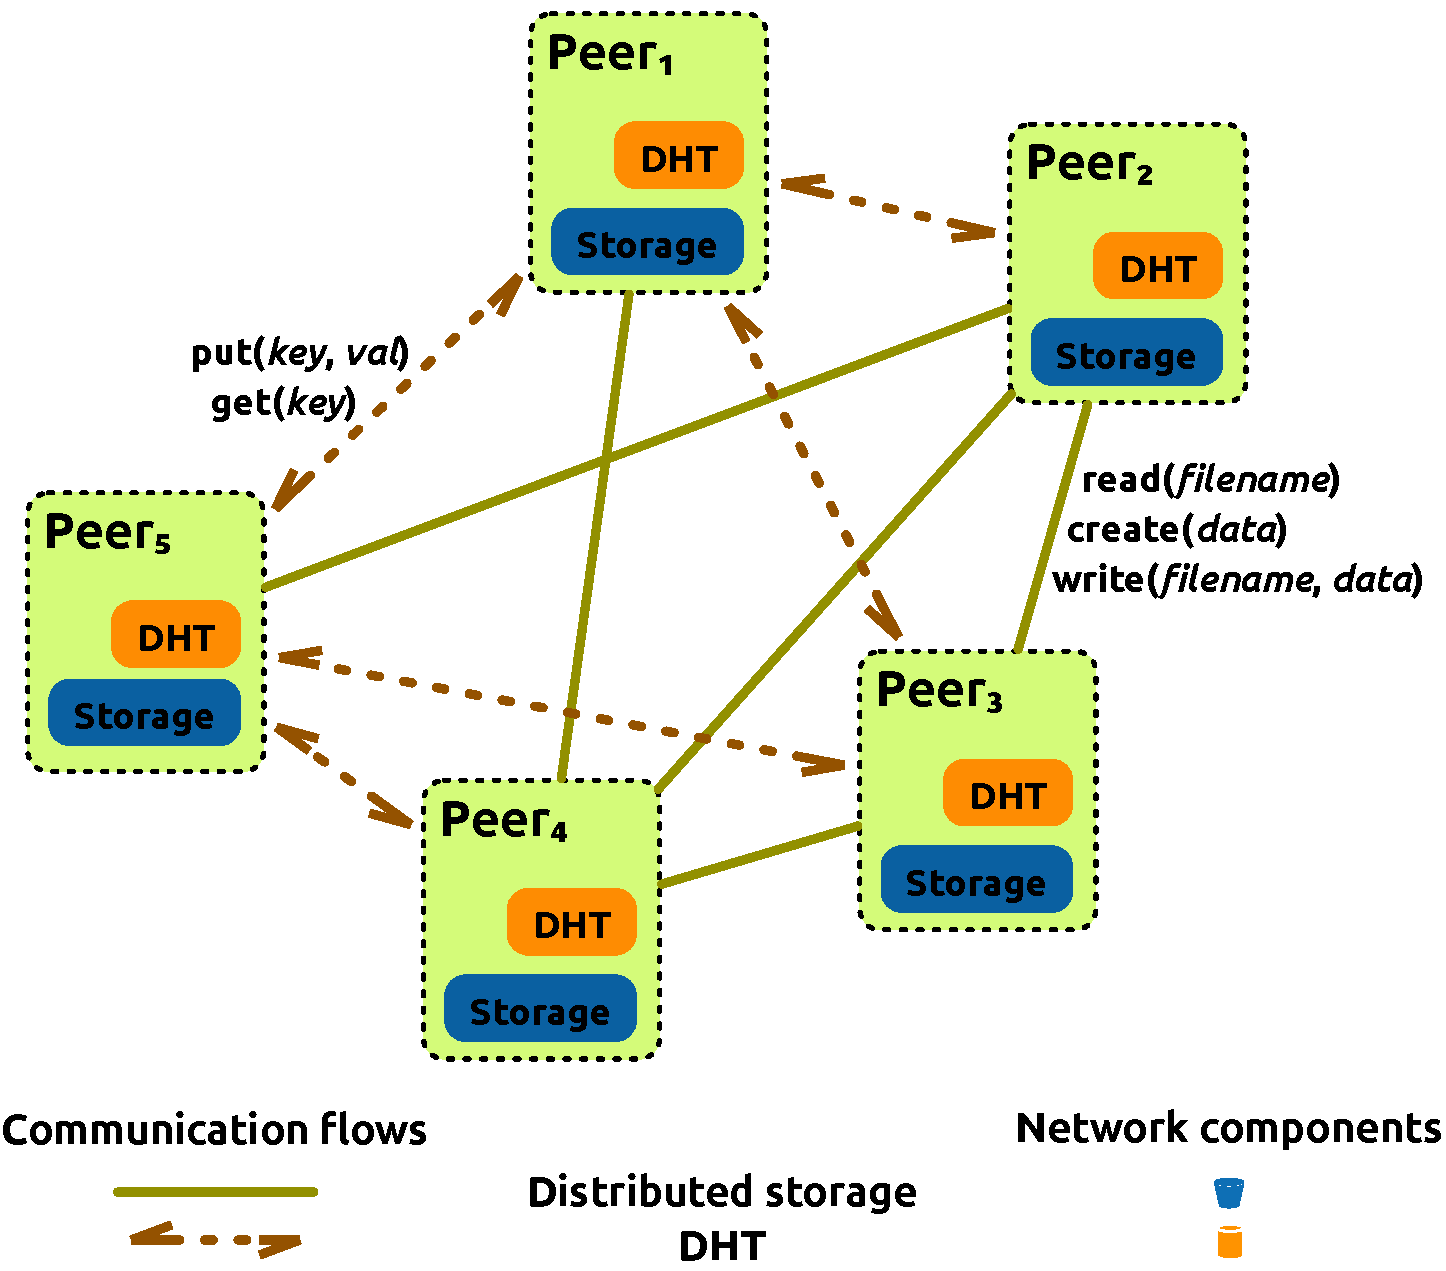
\includegraphics[width=.88\textwidth]{images/passwords-peer-to-peer/system-overview-fully-distributed}
  %\caption{System components. DHT is drawn separately for simplicity, but is
%also run on peers.}
  \caption{Overview of the system.}
  \figlabel{systemoverview}
\end{figure}

% sonja check if needed: that authenticates via cryptographic keys.
To make the system flexible across different implementations, we require as few non-standard features as
possible. The exception to this is the DHT that handles
account registration, mapping each registered username to a reference
in the storage.  For resilience against account hijacking,
we propose modifying the DHT to be write-once on keys:
once an account has been registered, nobody else can register that
username.

From the DHT we require two operations, \texttt{put}($key$, $value$), and
\texttt{get}($key$). The put operation associates the $value$ with the
$key$, and subsequent get operations on that $key$ will return the $value$.
As the DHT is write-once, a second put operation with the same $key$ will not
affect the system state.

The distributed storage functions for data
manipulation are similar to the DHT, with three
differences: we allow the distributed storage to select the ``filename'' for
us; we require that data can be updated; and we assume (minimalistic) access
control when writing. We refer to what is stored in the distributed storage as
files, to simplify our description. While the storage component
can be implemented as a distributed file system, we emphasize that our
requirements are significantly weaker than full file system semantics.

We formalize the API to the storage as having three
operations. First, \texttt{create}($data$) which generates a new file and
returns a filename. Second, \texttt{write}($filename$, $data$) that
overwrites the file $filename$ with content $data$. Third,
\texttt{read}($filename$) which reads the content from a file. Our security
does not require overwritten data to be inaccessible, so a solution
similar to GNUnet~\cite{Bennett03} or
Freenet~\cite{Clarke10} where a new version is stored and
pointed to suffice in our protocols.

We require the storage system to support some minimalistic access control.
Each stored file has an owner, which is the user who created the file.  Only
the owner can perform the \texttt{write} operation. To authenticate ownership
of files, we assume that a public-key cryptographic system is used.

Finally, for the peer sampling component, we require a \texttt{getPeer}() method,
returning a randomly selected peer, with a distribution close to uniform.

\section{Password-based P2P Login} \seclabel{passwordlogin}
For password-based authentication
in P2P systems, the basic functionality involved is registering an account,
and logging in. We also consider password change and remembered logins,
allowing a device to store sufficient information to log in %as a core component 
later without asking for credentials
anew. Following recommendations from the ISO 27002 standard~\cite{iso27002}, we define the
following requirements for our login procedure and add our
own (preceded by a star) to account for several devices.
\begin{itemize}
\item passwords should neither be stored nor transmitted in clear text
\item a user should be able to choose her own passwords and change them
\item files with passwords should be stored separately from application data 
\item[$\star$] a user should use the same password to log in from any device
\item[$\star$] it should not be possible to recover a password by stealing a
device with remembered credentials
\item[$\star$] it should be possible to block access to the account from a
stolen device
\end{itemize}
The standard also defines limitations for password login procedures
that our system cannot provide fully due to the lack of rate-limiting
possibilities in P2P networks: to limit the number of unsuccessful
login attempts and the maximum and minimum time allowed for the
login procedure.  Adapting a multi-party password hardening scheme
\cite{FordK00} could, in future work, be a way to achieve similar
properties in a P2P network. Besides this limitation, our protocols
fulfill the requirements as outlined in the standard, and our
own added requirements.
% According
%to the standard, \emph{the strength of user identification and authentication should be suitable to the sensitivity of the information to be accessed}.


% \textit{\textbf{ISO/IEC 27002:2005}} \\
% \textit{
% 11.5.1 Secure log-on procedures \\
% Access to operating system should be controlled by secure log-on procedure. ... A good log-on procedure should:
% }
% \textit{
% \begin{enumerate}
% \item not display system or application identifiers until the log-on procedure has been successfully completed;
% \item display a general notice warning that the computer should only be accessed by authorized users;
% \item not provide help messages during the log-on procedure that would aid an authorized user;
% \item validate the log-on information only on completion of all input data.If an error condition arises, the system should not indicate which part of the data is correct or incorrect;
% \item limit the number of unsuccessful log-on attempts allowed, e.g. to three attempts, and consider:
% \begin{enumerate}
% \item recording unsuccessful and successful attempts
% \item forcing a time delay before further log-on attempts are allowed or rejecting any further attempts without specific authorization
% \item disconnect data link connection
% \item sending an alarm message to the system console if the maximum number of log-on attempt is reached
% \end{enumerate}
% \item limit the maximum and minimum time allowed for the log-on procedure. If exceeded, the system should terminate the log-on;
% \item display the following information on completion of a successful log-on:
%  \begin{enumerate}
%  \item date and time of the previous successful log-on
%  \item details of any unsuccessful log-on attempts since the last successful log-on
% \end{enumerate}
% \item not display the password being entered or consider hiding the password characters by symbols;
% \item not transmit passwords in clear text over a network;
% \end{enumerate}
% }
% \textit{
% 11.5.2 User identification and authentication \\
% Other information}
% \textit{
% Passwords are a very common way to provide identification and authentication based on a secret that only the user knows. ... The strength of user identification and authentication should be suitable to the sensitivity of the information to be accessed.
% }

\begin{table}[htb]
\centering
\caption{Protocol Terminology}
\tablabel{terminology}
    \begin{tabular}{lp{5.92cm}}
 		\toprule
%		Designator & Description\\
%		\midrule
		$uname$ & Username\\
		$passwd$ & Password\\
		$salt$ & Random byte string\\
		$K_W$ & Cryptographic key for write authentication \\
		$F_{KS}$ & Key store file\\
		$f_{KS}$ & File name of $F_{KS}$\\
		$K_{KS}$ & Cryptographic key (used to encrypt $F_{KS}$)\\
		$F_{LI}, f_{LI}, K_{LI}$ & Login information file, its file name and key\\
		$F_{DL}, f_{DL}, K_{DL}$ & Device login information file, its file name and key\\
		$D, D_{ID}$ & User device and the identifier of $D$\\
		$K_{x1}, K_{x2}, \dots$ & Cryptographic keys for usage after logging in\\
		$devmap$ & Mapping from device identifiers to device login information files and corresponding keys\\
		\bottomrule
    \end{tabular}
\end{table}

We now describe our protocols based on the system model from
\secref{systemsoverview}.  \figref{loginProcedure} shows the
information objects and their storage locations, with arrows for the
abstract flow of the login procedure, \tabref{terminology} lists the terms
used in the algorithms.

\begin{figure}
  \centering
	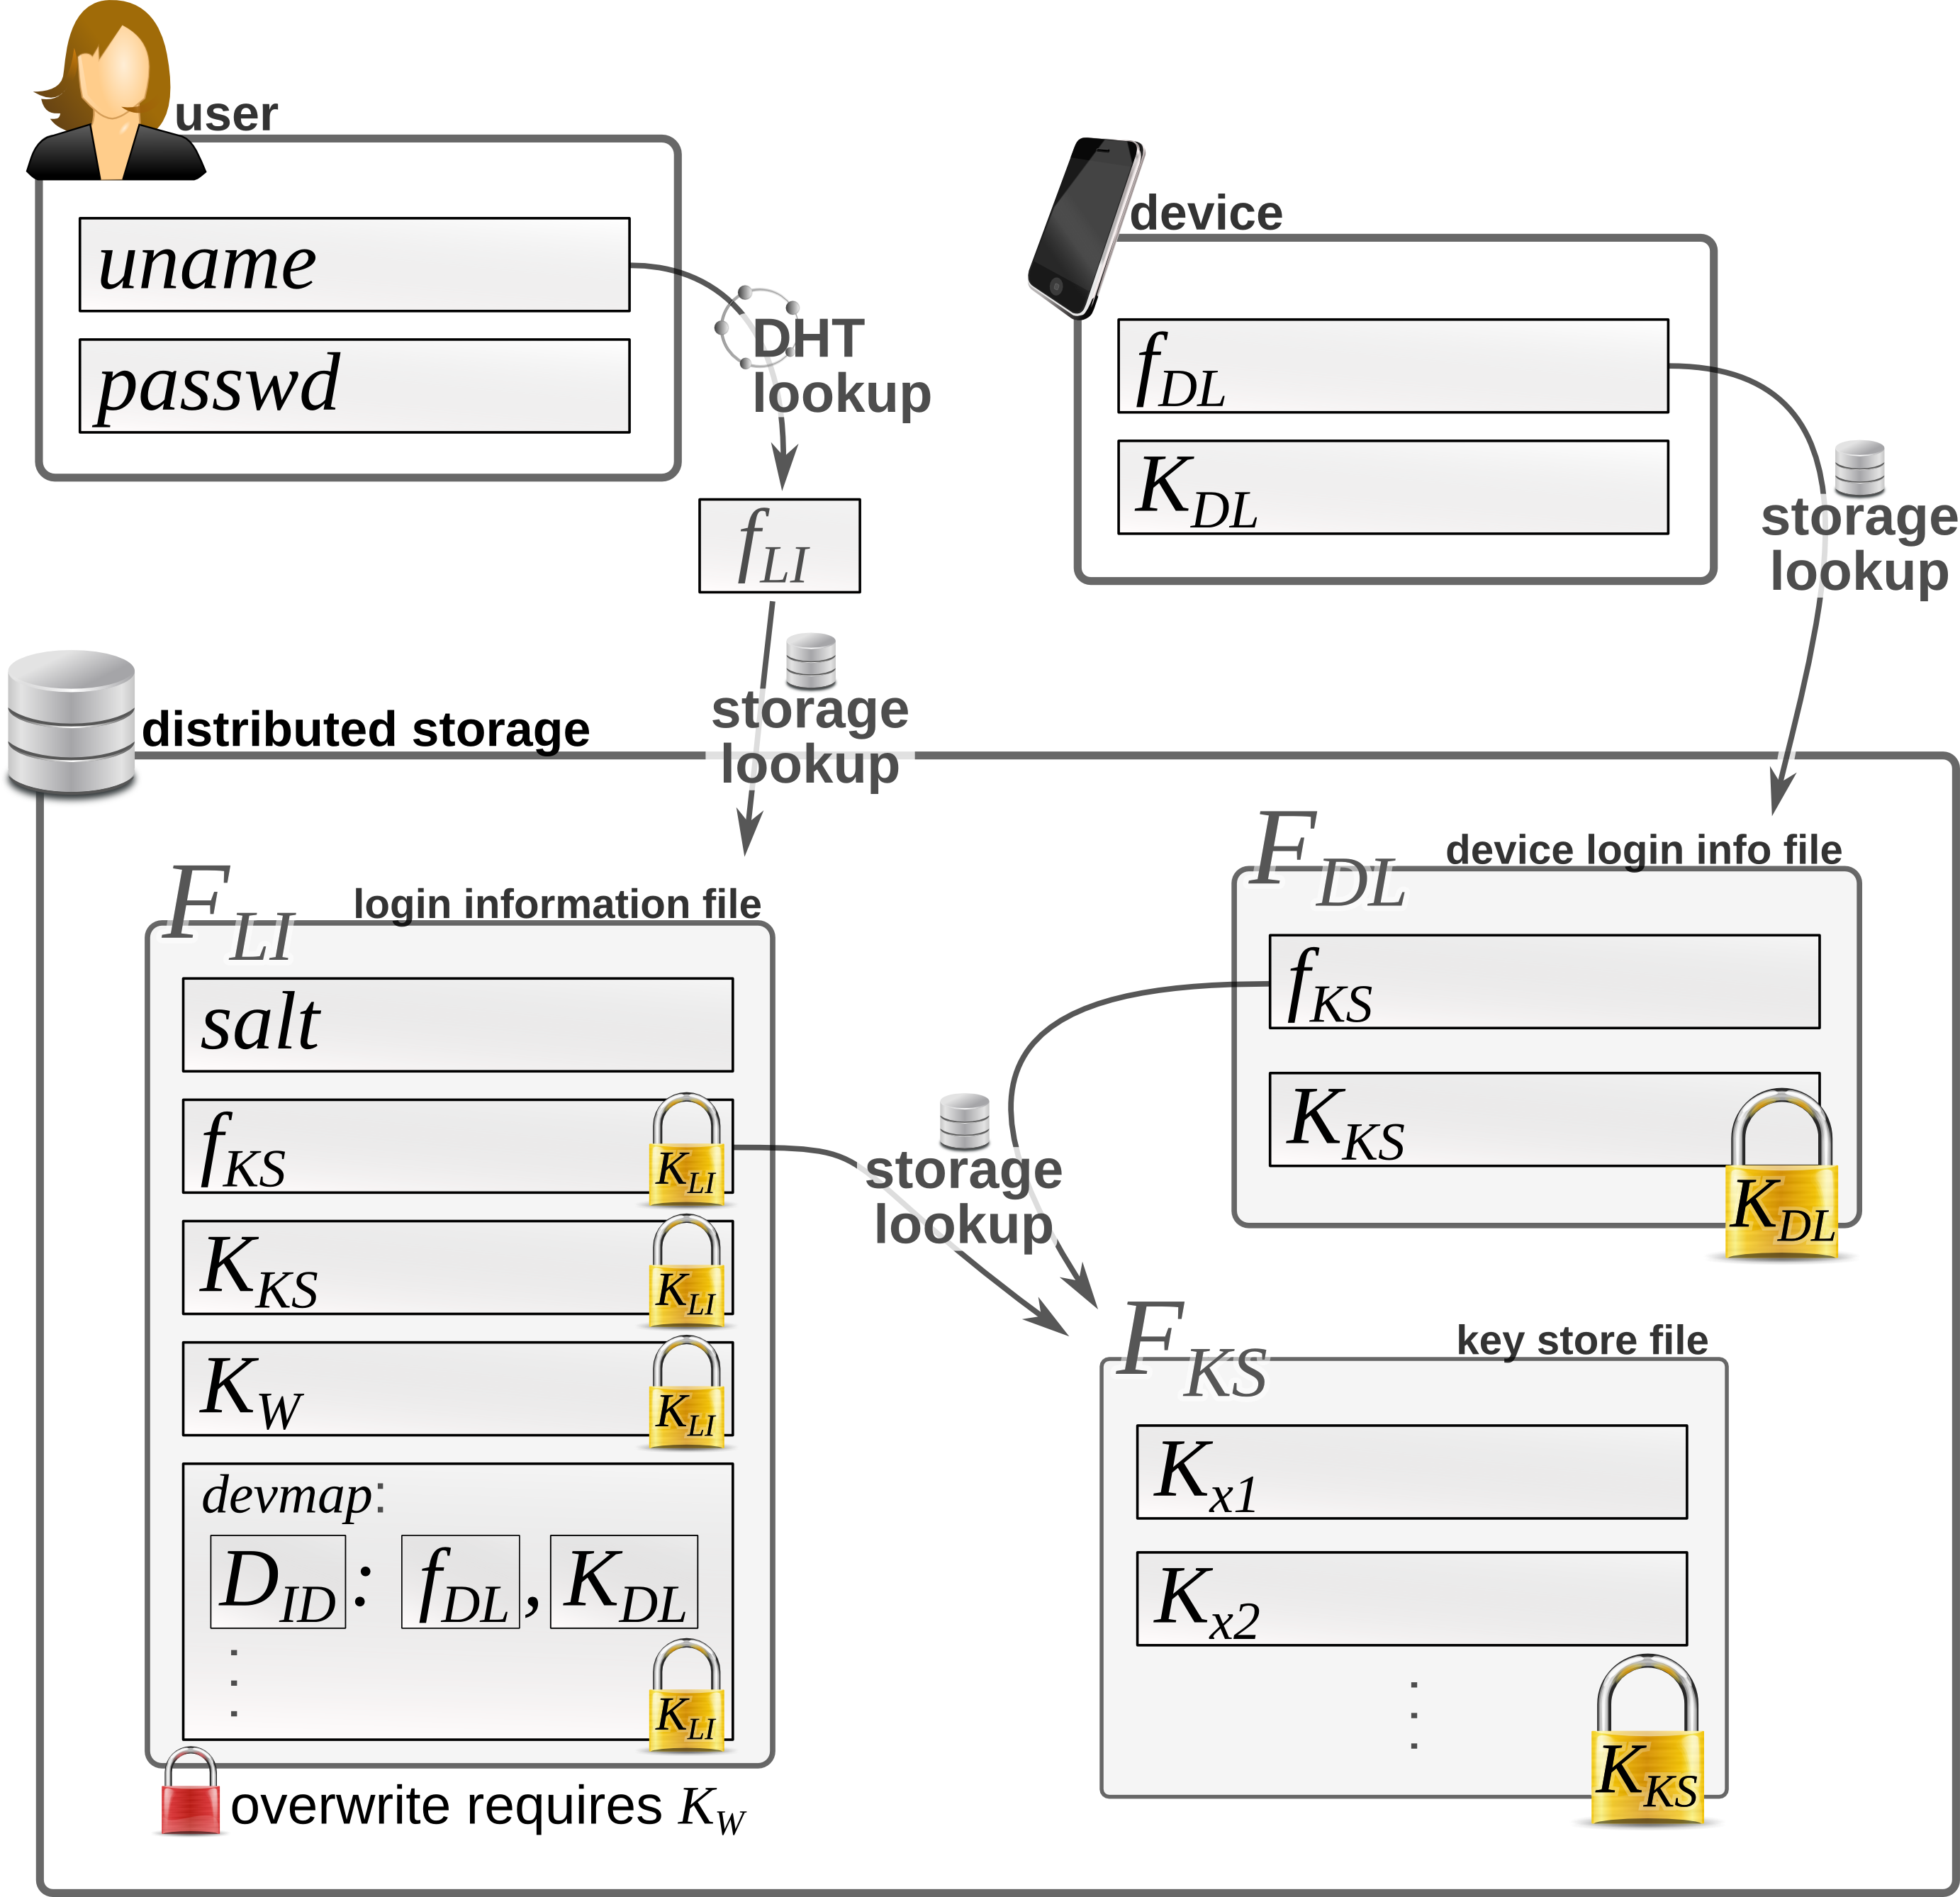
\includegraphics[width=.88\textwidth]{images/passwords-peer-to-peer/user-files-devices}
  \caption{Storage Locations (boxes) and Login Procedure (arrows)}
  \figlabel{loginProcedure}
\end{figure}

%% Pseudocode Definitions
% layout
\newcommand{\LineNumFrequency}{1} % 0 for no line numbers
\algrenewcommand{\algorithmiccomment}[1]{\hfill\textcolor{gray}{// #1}} % comment style
\algnewcommand\Input{\item[\textbf{Input:}]} % define \Input
\algnewcommand\Stored{\item[\textbf{Stored:}]} % define \Stored
% functions
\newcommand{\UserInput}[1]{User.input(``#1'')} % text
\newcommand{\DHTRead}[1]{DHT.get(#1)} % key
\newcommand{\DHTWrite}[2]{DHT.put(#1,#2)} % key, value
\newcommand{\StorageRead}[1]{Storage.read(#1)} % name
\newcommand{\StorageCreate}[1]{Storage.create(#1)} % value
\newcommand{\StorageWrite}[2]{Storage.write(#1,#2)} % name, value
\newcommand{\DeviceLocalRead}{Device.readLocalStore()}
\newcommand{\DeviceLocalWrite}[1]{Device.writeLocalStore(#1)} % value
\newcommand{\DeviceID}{Device.ID}
\newcommand{\NewKey}{generateKey()}
\newcommand{\NewSalt}{generateSalt()}
\newcommand{\NewMap}{createMap()}
\newcommand{\Encrypt}[2]{encrypt$_{#2}$(#1)} % plaintext, cryptkey (without $$)
\newcommand{\Decrypt}[2]{decrypt$_{#2}$(#1)} % ciphertext, cryptkey (without $$)
\newcommand{\KDF}[2]{KDF(#1,#2)} % salt, password
\newcommand{\NewShares}[3]{createShares(#1,#2,#3)} % n, m, plaintext
\newcommand{\UseShares}[1]{useShares(#1)} % shares
\newcommand{\GetPeer}{getPeer()}
\newcommand{\SendMail}[2]{sendMail(#1,#2)} % recipient, content

\subsection{Account Registration} \seclabel{accountregistration}

To register a new account (see \algoref{register}), the user first has to choose
a username $uname$ 
and a password $passwd$.
Next, the user creates a key store file $F_{KS}$, containing all the keys used 
by the P2P application the user wants to log in to (and an additional storage 
key, authenticating write operations on this file). %bgre: not mentioned in the code (if mentioned, it should also be included in the password change protocol)
The user then creates a symmetric key $K_{KS}$, encrypts the file content with this key and puts the ciphertext into the storage, obtaining a file name $f_{KS}$.
Now, the user creates a login information file $F_{LI}$ by creating a random byte string $salt$, deriving a symmetric key $K_{LI}$ from the password $passwd$ and the $salt$, encrypting $f_{KS}$, $K_{KS}$ and $K_W$ (a generated storage key, required for overwriting $F_{LI}$ later) with $K_{LI}$. The salt and the three encrypted values are put into the storage, obtaining a file name $f_{LI}$.
The salt is stored in plaintext, so that the user later can derive the decryption key $K_{LI}$ by only providing the password.
Finally, the user performs the write-once operation \texttt{put} on the DHT
with $uname$ as key and $f_{LI}$ as value. If the username was taken, the user
is prompted for a new username.
Once all operations have succeeded, the user is registered in the system.

\begin{algorithm}
\caption{Account Registration}
\algolabel{register}
% define Do-While construct
\algblockdefx{Do}{While}%
    {\textbf{do}}%
    [1]{\textbf{while} #1}
\begin{algorithmic}[\LineNumFrequency]
 \State $uname \gets$ \UserInput{Choose username:}
\State $passwd \gets$ \UserInput{Choose strong password:}
\State $K_{KS} \gets$ \NewKey % generate keystore key
\State $F_{KS} \gets$ \Encrypt{$K_{x1}||K_{x2}||\dots$}{K_{KS}} % encrypt key material to be stored in key store
\State $f_{KS} \gets$ \StorageCreate{$F_{KS}$} % no need for a storage authenticating key here, because we never need to overwrite this file again (we create new ones instead)
\State $salt \gets$ \NewSalt
\State $devmap \gets$ \NewMap %bgre: for metadata-privacy reasons a new ``empty'' map should consist of a couple of dummy entries
\State $K_{LI} \gets$ \KDF{$salt$}{$passwd$}
\State $K_W \gets$ \NewKey \Comment{suitable for the storage system} % or even provided by the storage system component
\State $F_{LI} \gets salt || $\Encrypt{$f_{KS}||K_{KS}||K_W||devmap$}{K_{LI}}
\State $f_{LI} \gets$ \StorageCreate{$F_{LI}$}\Comment{using $K_W$} %setting ownership using $K_W$
\While{\DHTWrite{$uname$}{$f_{LI}$} fails}
    \State $uname \gets$ \UserInput{Choose new username:}
\EndWhile
\end{algorithmic}
\end{algorithm}


\subsection{Login} \seclabel{loginprotocol}

Once registered, a user is able to log in -- that is, to retrieve the
cryptographic keys stored in the key store file $F_{KS}$ -- 
from any device by only entering her username and password (see \algoref{login}).
%
A \texttt{get} request with the parameter $uname$ to the DHT results in the 
filename $f_{LI}$ for the login information file $F_{LI}$. 
This file is retrieved from the distributed storage and contains the $salt$ in plaintext.
The latter is fed into a key-derivation function together with the user password to derive the key $K_{LI}$.
This key allows the user to decrypt all other content of the login information file,
including the filename $f_{KS}$ of the key store file and the corresponding key $K_{KS}$.
Finally, the user fetches the key store file $F_{KS}$ from the storage system 
and decrypts it, using $K_{KS}$. 
This concludes the login procedure as the user is now in possession
of the keys $K_{x1}, K_{x2}, \dots$, required by the P2P application.

If the user chose to remember the login information on the local device,
a new device login information file $F_{DL}$ is created and saved to the storage system
(which returns a filename $f_{DL}$). This file contains the filename
$f_{KS}$ of the key store file as well as the according key $K_{KS}$ and is encrypted
with a new key $K_{DL}$. On the device, only the filename $f_{DL}$ and the key $K_{DL}$
are stored locally.
Additionally, a reference to the device login information file is stored in the $devmap$ value
of the login information file $F_{LI}$. It contains a mapping from a device identifier to the filename
and key of the device login information file, allowing password changes and device revocation 
as described later.

When the user wants to log in from the same device again, the
locally stored values ($f_{DL}, K_{DL}$) are used to retrieve the device login
information file, decrypt it, and thereby gain access to the key store
file. Thus, the remembered login feature allows the user to log in
without entering the password, while nothing password-related is
stored on the device. Furthermore, remembered logins remain valid
even if the P2P application changes keys in the key store file.

\begin{algorithm}
\caption{Login}
\algolabel{login}
\begin{algorithmic}[\LineNumFrequency]
\State $f_{DL},K_{DL} \gets$ \DeviceLocalRead
\If {$f_{DL} \neq$ \texttt{NULL}} \Comment{non-interactive login}
   \State $F_{DL} \gets$ \StorageRead{$f_{DL}$}
   \State $f_{KS},K_{KS} \gets$ \Decrypt{$F_{DL}$}{K_{DL}}
   \State $saveLoginLocally \gets$ \texttt{False}
\Else \Comment{interactive login}
   \State $uname \gets$ \UserInput{Enter username:}
   \State $passwd \gets$ \UserInput{Enter password:}
   \State $saveLoginLocally \gets$ \UserInput{Remember?}
   \State $f_{LI} \gets$ \DHTRead{$uname$}
   \State $F_{LI} \gets$ \StorageRead{$f_{LI}$}
   \State $salt \gets F_{LI}.salt$ \Comment{stored in plaintext} 
   \State $K_{LI} \gets$ \KDF{$salt$}{$passwd$}
   \State $f_{KS}, K_{KS}, K_W, devmap \gets$ \Decrypt{$F_{LI}$}{K_{LI}}
\EndIf

\State $F_{KS} \gets$ \StorageRead{$f_{KS}$}
\State $K_{x1},K_{x2},\dots \gets$ \Decrypt{$F_{KS}$}{K_{KS}}

\If {$saveLoginLocally$}
   \State $K_{DL} \gets$ \NewKey
   \State $F_{DL} \gets$ \Encrypt{$f_{KS} || K_{KS}$}{K_{DL}}
   \State $f_{DL} \gets$ \StorageCreate{$F_{DL}$}
   \State \DeviceLocalWrite{$f_{DL} || K_{DL}$}
   \State $devmap$.append(\DeviceID, $f_{DL} || K_{DL}$)
   \State $F_{LI} \gets salt || $\Encrypt{$f_{KS}||K_{KS}||K_W||devmap$}{K_{LI}}
   \State \StorageWrite{$f_{LI}$}{$F_{LI}$} \Comment{using $K_W$}
\EndIf

\end{algorithmic}
\end{algorithm}

\subsection{Password Change} \seclabel{pwchangeprotocol}
Before the user can change the password, she must log in using her password to obtain $K_{LI}$.
With this information, the password change can be accomplished (see
\algoref{passwordChange}): the user is asked for a new password and a new salt is generated. The key-derivation function is used to generate a new key $K_{LI}^{new}$ for the login information file. Then, the content of the key-store file is fetched and decrypted (with the old key). A new key $K_{KS}^{new}$ is generated and used for encrypting the key-store content again before it is saved to the storage system, obtaining a new filename $f_{KS}^{new}$. Finally, the login information file is updated: $f_{KS}^{new}, K_{KS}^{new}$, the write credential $K_W$ as well as a new empty device mapping $devmap^{new}$ are encrypted with the new key $K_{LI}^{new}$. Together with the new salt, this ciphertext is written to the distributed storage, using the reference $f_{LI}$ and the credential $K_W$, to authenticate the \texttt{write} operation.
Lastly, the keys stored in the key store should be updated by the application
using our P2P protocol. See \secref{refreshkeystore} for a discussion. At this
point, old device login information files can also be deleted from the storage to
reclaim space.

\begin{algorithm}
\caption{Password Change}
\algolabel{passwordChange}
\begin{algorithmic}[\LineNumFrequency]
\Input $uname, K_{LI}^{old}$
% \State $uname \gets$ \UserInput{Enter username:}
% \State $K_{LI}^{old} \gets$ recovery($uname$) % the recovery function will ask for more user input (e-mail or security-questions)
\State $f_{LI} \gets$ \DHTRead{$uname$}
\State $F_{LI}^{old} \gets$ \StorageRead{$f_{LI}$}
\State $f_{KS}^{old},K_{KS}^{old},K_W,devmap^{old} \gets$ \Decrypt{$F_{LI}^{old}$}{K_{LI}^{old}} 
\State $passwd^{new} \gets$ \UserInput{Enter new password:}
\State $salt^{new} \gets$ \NewSalt
\State $K_{LI}^{new} \gets$ \KDF{$salt^{new}$}{$passwd^{new}$}
\State $devmap^{new} \gets$ \NewMap

\State $F_{KS}^{enc-old} \gets$ \StorageRead{$f_{KS}^{old}$}
\State $F_{KS} \gets$ \Decrypt{$F_{KS}^{enc-old}$}{K_{KS}^{old}}
\State $K_{KS}^{new} \gets$ \NewKey
\State $F_{KS}^{enc-new} \gets$ \Encrypt{$F_{KS}$}{K_{KS}^{new}}
\State $f_{KS}^{new} \gets$ \StorageCreate{$F_{KS}^{enc-new}$} % overwriting the old file (instead of creating a new one) would break the transactional property of this operation 
\State $F_{LI}^{new} \gets$
\Statex $salt^{new} ||$ \Encrypt{$f_{KS}^{new}||K_{KS}^{new}||K_W||devmap^{new}$}{K_{LI}^{new}}
\State \StorageWrite{$f_{LI}$}{$F_{LI}^{new}$} \Comment{using $K_W$}
\State Refresh keys stored in key store
\State Old device login information files may be deleted
\end{algorithmic}
\end{algorithm}


% \begin{algorithm}
% \caption{Password Change} % implies logging out all remembered devices
% \algolabel{passwordChange}
% \begin{algorithmic}[\LineNumFrequency]
% \State $uname \gets$ \UserInput{Enter username:}
% \State $passwd^{old} \gets$ \UserInput{Enter old password:}
% 
% % LOGIN($uname, passwd^{old}$) >>> $K_W,K_{KS},f_{KS}$ 
% \State $f_{LT} \gets$ \DHTRead{$uname$}
% \State $F_{LI} \gets$ \StorageRead{$f_{LI}$}
% \State $salt \gets F_{LI}.salt$ \Comment{stored in plaintext} 
% \State $K_{LI} \gets$ \KDF{$salt$}{$passwd$}
% \State $f_{KS}^{old}, K_{KS}^{old}, K_W, devmap \gets$ \Decrypt{$F_{LI}$}{K_{LI}}
% 
% % \State $passwd^{new} \gets$ \UserInput{Enter new password:") 
% 
% % RESET-PASSWD($uname, passwd^{new}$)
% \State ...\Comment{continue with ``Password Reset'' protocol in line~3}
% \end{algorithmic}
% \end{algorithm}


\subsection{Logout} \seclabel{logoutprotocol}

To log out from the system, the user does not have to interact with the DHT or
the storage system.  Simply wiping her local cache from application data and
all key material restores the pre-login state.  If the user chose to
remember the login on a device, the corresponding device login information
file $F_{DL}$ can also be deleted from
the storage. % bgre: we need a K_W here for overwriting, how do we get it? Or we create a new credential for each F_DL that we store locally as well (and in the devmap).
%bgre: We can not delete the entry in the devices-mapping in F_LI, because we do not have K_LI to modify this field (asking the user for the password for a simple logout would not be convenient),
% so we leave it in and garbage collect it the next time, when it would be used (a garbage entry is one that can not be decrypted by the K_DL stored in the mapping)

A problem related to logging out is revoking remembered credentials on another
device, \eg a user's stolen phone.
To accomplish this, we first run the password change operation, which 
locks out all devices with remembered logins, because the key store key $K_{KS}$
changed (as well as the filename $f_{KS}$).
Next, we use the device mapping $devmap$ to inform all devices about the
new key (and filename), except the device that is to be revoked. To
inform a device about the change, we update the corresponding values in the device's
login information file $F_{DL}$ which can be accessed from the device by using
the locally stored credentials.

\algoref{logoutOtherDevice} describes this necessary extension.  
After running the password change operation, all devices that should \emph{not} 
be revoked and that have remembered logins (and therefore are 
referenced in the device mapping $devmap$) are processed.
The device login information filename $f_{DL}$ and its key $K_{DL}$ 
are read, and the new key store key $K_{KS}^{new}$ and filename $f_{KS}^{new}$ 
are written to the device login information file $F_{DL}$, encrypted under the 
device key $K_{DL}$. Finally, the modified $devmap$ is saved back to the 
login information file $F_{LI}$.

% We remark that device revocation addresses the problem when a user's device is
% lost. It does not help in case the user has entered her credentials into a
% malicious device, as such a device can store her username and password
% directly.
% \todo{bgre: This paragraph is a bit misleading, because a password change is 
%             part of the logout operation (not necessary but in our protocol),
%             so it is more a race between the malicious device and the user 
%             (who changes password first, wins). So, maybe delete this paragraph 
%             here and say something about the race issue in the security 
%             evaluation instead?}

\begin{algorithm}
\caption{Logout Other Device} % implies changing the password
\algolabel{logoutOtherDevice}
% define For-Each construct
\algblockdefx{Foreach}{Endforeach}%
    [2]{\textbf{foreach} #1 \textbf{in} #2}%
    {\textbf{end}}
\begin{algorithmic}[\LineNumFrequency]
\State ... \Comment{run \algoref{passwordChange} (Password Change)}
\State $deviceToLogout \gets$ \UserInput{Select device:}
\State $devmap.remove(deviceToLogout)$
\Foreach {$D_{ID}$}{$devmap$} \Comment{all devices to keep}
  \State $f_{DL},K_{DL} \gets$ $devmap$.get($D_{ID}$)
  \State $F_{DL} \gets$ \Encrypt{$f_{KS}^{new}||K_{KS}^{new}$}{K_{DL}}
  \State \StorageWrite{$f_{DL}$}{$F_{DL}$}
\Endforeach
\State ... \Comment{save modified $devmap$ back to $F_{LI}$}
\end{algorithmic}
\end{algorithm}

\section{Password Recovery} \seclabel{recovery} An important part of
password-based logins is the possibility for users to recover their
accounts if they forget their passwords. We refer to this as a
\emph{password recovery mechanism}. The goal of a password recovery
mechanism is to provide a secondary way of authenticating the
user. There are a number of password recovery mechanisms used in
practice. In our experience, three of the most common ones are
password hints, security questions, and e-mail based recovery. Other
approaches (beyond the scope of this paper) include vouching for identity by
social contacts~\cite{Brainard06}, or using trusted devices.
% \begin{itemize}
% \item Password hints
% \item Security questions
% \item E-mail based password recovery
% \end{itemize}

Password hints means that the user may enter a hint at the same time as she
sets this password. The hint will be displayed to her if she forgets her
password, and should be selected such that it helps her recall her password,
but does not make it significantly easier for someone else to guess it. The
hint is not truly a secondary authentication mechanism, but rather a means to
recovering the original password-based authentication mechanism. A basic 
version of password hints would be straightforward to implement in our system: 
the hint can be stored in plaintext in the login information file. 
Security questions and e-mail based password recovery are more complex to adapt.
We described their implementation in detail after listing requirements.

As in \secref{passwordlogin} for the login procedure, we  define a set of functional
requirements for password recovery, based on the ISO 27002 standard~\cite{iso27002} as follows. We
also augment the list with requirements of our own (preceded by a star).

\begin{itemize}
	\item establish methods to verify the identity of a user prior to allowing the user to choose a new password
	\item communicate with those affected by or involved with recovery security incidents 
	\item have procedures to allow recovery and restoration of business operations and availability of information in a time-scaled manner 
	\item a legitimate user should be able to recover lost (forgotten) or broken (device's) keys
	\item[$\star$] the recovery procedure should allow a user to set a new password, not reveal the old password
	\item[$\star$] the process of recovery should be easy to use
	\item[$\star$] sensitive information for recovery should be kept secret
\end{itemize}
Our protocols support these requirements. The sole exception is that if a
password is reset via security questions alone, the system would not
``communicate with those affected'' (e.g., send an e-mail notification that
the password had been reset, as is common in centralized services).
We remark that the last item is a stronger property than many
centralized systems provide. In our system, no one learns the
answers to a user's security questions. We consider this to be
important, since many systems use similar security questions.

The operations described in this section imply minor additions to the protocols
of \secref{passwordlogin}, \ie invoking the update procedures after each password change
(to sustain transaction safety, the updates have to be included in the final write operation of
the password change operation).

% \textit{Some properties of interest for password recovery to argue, discuss, include,...:
% \begin{itemize}
% 	\item Entropy
% 	\item Fault-tolerance (what happens with the chosen peers over time... for instance, if they don't ever log in back, we could run into the situation of having less `still-active' peers than the minimum we require to perform the recovery) Check paper: \url{http://dl.acm.org/citation.cfm?id=501985}
% 	\item Minimize delay when recovering (password hint is presumably the fastest one for instance). This is related to evaluation... disaster scenario
% 	\item Collision avoidance. This is related to the distribution of the peers chosen, we now say that it should be almost uniform, but how do we guarantee that? \todo{Look for reference on P2P systems and see how they choose peers to avoid these problems}
% 	\item Usability (minimize complexity for the user, for instance choosing the random peers when using the email recovery could be a hassle...). Unlikely that this one goes in, but found this paper on adaptability of the questions... \url{http://www.comp.lancs.ac.uk/iwssi2007/papers/iwssi2007-04.pdf} \todo{Use this paper also for evaluation, it has details about attacks}
% %Maybe this one too: http://www.sciencedirect.com/science/article/pii/S0167404807001083
% \end{itemize}
% }

\begin{table}[htb]
\centering
\caption{Recovery Protocol Terminology}
\tablabel{recoveryTerminology}
    \begin{tabular}{lp{65mm}}
		\toprule
% 		Designator & Description\\	
% 		\midrule
		\multicolumn{2}{c}{Security Question Recovery}\\
		\midrule
		$qS_i $ & ($n,k$)-secret sharing share of $K_{LI}$\\
		$Q_i $ & Security challenge question\\
		$A_i $ & Answer to question $Q_i$\\
		$qsalt_i $ & Random byte string \\
		$qK_i $ & Key to encrypt the share $qS_i$\\
		\midrule
		\multicolumn{2}{c}{E-mail Based Recovery}\\
		\midrule
		$K_R $ & Long-term recovery key\\
		$eS_i $ & ($n,k$)-secret sharing share of $K_R$\\
		$email $ & Recovery e-mail address of the user\\
		$peer_i $ & Randomly selected peer\\
		$esalt_i $ & Random byte string (to seed the e-mail commitment)\\
		$ksalt_i $ & Random byte string (to seed the key $eK_i$)\\
		$C_i $ & Cryptographic commitment to the e-mail address\\
		$eK_i $ & Key to encrypt the share $eS_i$\\
		\bottomrule
    \end{tabular}
\end{table}

\subsection{Security Questions}

Security questions is a password recovery technique
that relies on answers to questions the user is asked during registration.
The answers should be such that they cannot be easily guessed or researched by an attacker, but
still stable over time, memorable, and definite~\cite{GoodSecurityQuestions}.
Rabkin~\cite{Rabkin08} underlines the importance to choose good questions especially in the era of social networks.
Frykholm and Juels~\cite{FrykholmJ01} discuss a related technique that is similar to 
our adaption of this scheme.  

% One popular technique in centralized systems when a user creates a new account is asking the user with a set of questions such that in the hypothetical case that the user forgets its account password she is still able to regain access to the account by setting up a new password once the answers to those questions asked during registration match to the answers given during registration.

% \textit{This technique, called "Challenge questions" is discussed in the FFIEC supplement to the "Authentication in an Internet Banking Environment" guidance. Ordinary challenge questions are not considered adequate due to the amount of information about people on the Internet, but sophisticated, “out of wallet” questions provide an "effective component of a layered security".}

We assume that the user provides $n$
answers $A_i$ to suitable security questions $Q_i$. In order to recover the password, we 
require the user to answer any $k$ out of these $n$ questions correctly. 
The choice of $k$ constitutes an obvious trade-off between security and usability.
A successful recovery yields the key $K_{LI}$ to the login information file, allowing
the user to change the password, using \algoref{passwordChange}.
Our implementation does not require the user to provide new answers
after a regular password change. Additionally, we avoid storing the plaintext answers to the security questions.

For the setup of the question based recovery mechanism (\algoref{questionSetup}), we first create $n$ 
shares $qS_1, \dots, qS_n$ of the key $K_{LI}$ under an ($n,k$)-secret sharing scheme. For each
of these shares, we create a salt $qsalt_i$, derive a key $qK_i$ from this salt and the
answer $A_i$, and use it to encrypt the share, yielding $qS_i^{enc}$. Furthermore we encrypt the key $qK_i$
with the login information file key $K_{LI}$, for the update procedure described later.
Finally, the login information file is extended with all questions $Q_i$, the salts $qsalt_i$, the encrypted
shares $qS_i^{enc}$ and the encrypted keys $qK_i^{enc}$. When recovering, the
user has to reproduce at least $k$ answers, which together with the stored
salts can be used to derive $k$ keys $qK_i$, which in turn can decrypt $k$
shares $qS_i$.

When $K_{LI}$ changes (\eg due to a regular password change), we update the recovery information
as in \algoref{questionUpdate}: for the new key $K_{LI}^{new}$, a new set of shares is created.
Next, the keys $qK_i$ are decrypted and used to encrypt the new shares. Neither the keys
$qK_i$ nor the salts $salt_i$ change, so the user can still use the same answers for recovery. Finally, the updated
shares (and re-encrypted keys, to allow further updates) are saved back to the login information file.

\begin{algorithm}
\caption{Security Questions Setup}
\algolabel{questionSetup}
\begin{algorithmic}[\LineNumFrequency]
\State $qS_1,\dots,qS_n \gets$ \NewShares{$n$}{$k$}{$K_{LI}$} 
\For{$i \gets 1, n$}
  \State $Q_i \gets$ \UserInput{Enter question $i$:}
  \State $A_i \gets$ \UserInput{Enter answer $i$:}
  \State $qsalt_i \gets$ \NewSalt
  \State $qK_i \gets$ \KDF{$qsalt_i$}{$A_i$}
  \State $qS_i^{enc} \gets$ \Encrypt{$qS_i$}{qK_i}
  \State $qK_i^{enc} \gets$ \Encrypt{$qK_i$}{K_{LI}}
\EndFor
\State add to $F_{LI}$: $qS_i^{enc},qK_i^{enc}$ and the plaintext values of $Q_i,qsalt_i \quad\forall i \in \{1,\dots,n\}$ 
\end{algorithmic}
\end{algorithm}

\begin{algorithm}
\caption{Security Questions Update (on $K_{LI}$ change)}
\algolabel{questionUpdate}
\begin{algorithmic}[\LineNumFrequency]
\State $qS_1^{new},\dots,qS_n^{new} \gets$ \NewShares{$n$}{$k$}{$K_{LI}^{new}$}
\For{$i \gets 1, n$}
  \State $qK_i \gets$ \Decrypt{$qK_i^{enc}$}{K_{LI}}
  \State $qS_i^{new-enc} \gets$ \Encrypt{$qS_i^{new}$}{qK_i}
  \State $qK_i^{new-enc} \gets$ \Encrypt{$qK_i$}{K_{LI}^{new}}
\EndFor
\State update in $F_{LI}$: $qS_i^{new-enc},qK_i^{new-enc} \quad\forall i \in \{1,\dots,n\}$ 
\end{algorithmic}
\end{algorithm}

\subsection{E-mail Based}

In e-mail based password recovery, the user is sent an e-mail
containing some information, typically a link with a token, by which she can
reset her password. This link is sent to an e-mail address she has registered
with her account.

We adapt this scheme by randomly choosing a number of peers, that collaboratively provide this
functionality to the user. We use ($n,k$)-secret sharing 
to enable password recovery even if not all of the involved peers are online
when the user wants to recover the password. We discuss parameter choices of $k$ and $n$
in \secref{evalemail}.

To provide persistence of the recovery mechanism independent of a changing key $K_{LI}$ 
(\eg due to a password change), the result of the recovery process is a 
recovery key $K_R$, that always encrypts the current version of $K_{LI}$. 
\algoref{emailSetup} describes the setup procedure: 
From the recovery key $K_R$, $n$ shares $eS_1,\dots,eS_n$ are generated using ($n,k$)-secret
sharing. For each share, a random peer $peer_i$ is picked, two salts $esalt_i$ and $ksalt_i$ are created and a cryptographic commitment $C_i$
is derived from the salt $esalt_i$ together with the $email$. This commitment will be used to authorize the
user to the peer, and bind it to this specific e-mail address. 
Next, a key $eK_i$, to encrypt the share $eS_i$, is derived in the same way as the commitment, 
but with salt $ksalt_i$. 
A different salt is needed so that the peer cannot decrypt the share (before learning the address).
The commitment and the encrypted share are stored at the peer. The login information $F_{LI}$ file is extended
with a list of the chosen peers $peer_i$ and the according salts $esalt_i$, $ksalt_i$, as well as $K_{LI}^{enc}$,
encrypted with the recovery key, and the recovery key, encrypted with $K_{LI}$ (to allow for password changes).


\begin{algorithm}
\caption{E-mail Recovery Setup}
\algolabel{emailSetup}
\begin{algorithmic}[\LineNumFrequency]
\State $K_R \gets$ \NewKey \Comment{long-term recovery key}
\State $K_{LI}^{enc} \gets$ \Encrypt{$K_{LI}$}{K_R}
\State $eS_1,\dots,eS_n \gets$ \NewShares{$n$}{$k$}{$K_R$} 
\State $email \gets$ \UserInput{Enter recovery e-mail address:}
\For{$i \gets 1, n$}
  \State $peer_i \gets$ \GetPeer
  \State $esalt_i \gets$ \NewSalt
  \State $ksalt_i \gets$ \NewSalt
  \State $C_i \gets$ \KDF{$esalt_i$}{$email$} \Comment{commitment}
  \State $eK_i \gets$ \KDF{$ksalt_i$}{$email$}
  \State $eS_i^{enc} \gets$ \Encrypt{$eS_i$}{eK_i} % share-holders can only collude after the user revealed its email address
  \State store at $peer_i$: $C_i, eS_i^{enc}$  
\EndFor
\State $K_R^{enc} \gets$ \Encrypt{$K_R$}{K_{LI}}
\State add to $F_{LI}$: $K_{LI}^{enc}, K_R^{enc}$ and the plaintext values of $peer_i, esalt_i, ksalt_i \quad\forall i \in \{1,\dots,n\}$ 
\end{algorithmic}
\end{algorithm}


To recover the password (\algoref{emailUser}), the user looks up the available
information in the login information file, including the list of peers 
to be requested for assistance.
Each request is authorized by the commitment $C_i$, that the peer can derive
from the salt $esalt_i$ and the e-mail address, that the user provided (\algoref{emailPeer}).
If the request was legitimate, the peer sends the encrypted share to the e-mail address.
As soon as the user collected $k$ answers, she can recover $K_{LI}$.

\begin{algorithm}
\caption{E-mail Recovery: User}
\algolabel{emailUser}
\begin{algorithmic}[\LineNumFrequency]
\State $uname \gets$ \UserInput{Enter username:}
\State $email \gets$ \UserInput{Enter e-mail:}
\State $f_{LI} \gets$ \DHTRead{$uname$}
\State $F_{LI} \gets$ \StorageRead{$f_{LI}$}
\State $K_{LI}^{enc}; \forall i: peer_i, esalt_i, ksalt_i \gets F_{LI}$ \Comment{plaintext part}
% \State $K_{LI}^{enc}, peer_{1,\dots,n}, esalt_{1,\dots,n}, ksalt_{1,\dots,n} \gets F_{LI}$ \Comment{plaintext part}
\State $\forall i:$ send $(email, esalt_i)$ to $peer_i$ \Comment{send $n$ requests}
\State $eS_1^{enc},\dots,eS_k^{enc} \gets$ read e-mail \Comment{wait for $k$ e-mails}
\For{$i \gets 1, k$}
  \State $eK_i \gets$ \KDF{$ksalt_i$}{$email$}
  \State $eS_i \gets$ \Decrypt{$eS_i^{enc}$}{eK_i}
\EndFor
\State $K_R \gets$ \UseShares{$eS_1,\dots,eS_k$}
\State $K_{LI} \gets$ \Decrypt{$K_{LI}^{enc}$}{K_R}
\State ...\Comment{run \algoref{passwordChange} (Password Change)}
\end{algorithmic}
\end{algorithm}

\begin{algorithm}
\caption{E-mail Recovery: Peer}
\algolabel{emailPeer}
\begin{algorithmic}[\LineNumFrequency]
\Stored $C_i, eS_i^{enc}$ \Comment{stored at peer}
\Input $email, esalt_i$ \Comment{provided by the user request} % note that still the peer cannot decrypt the share, because it does not have ksalt_i to derive eK_i
\If {$C_i =$ \KDF{$esalt_i$}{$email$}} \Comment{legitimate request}
  \State \SendMail{$email$}{$eS_i^{enc}$}
\EndIf
\end{algorithmic}
\end{algorithm}

To provide long-term persistence of this recovery mechanism,
$K_{LI}^{enc}$ has to be updated whenever $K_{LI}$ changes. 
\algoref{emailUpdate}
describes the necessary steps, including updating
$K_R^{enc}$ to allow subsequent updates.

\begin{algorithm}
\caption{E-mail Recovery Update (on $K_{LI}$ change)}
\algolabel{emailUpdate}
\begin{algorithmic}[\LineNumFrequency]
\State $K_R \gets$ \Decrypt{$K_R^{enc}$}{K_{LI}^{old}} 
\State $K_{LI}^{enc-new} \gets$ \Encrypt{$K_{LI}^{new}$}{K_R}
\State $K_R^{enc-new} \gets$ \Encrypt{$K_R$}{K_{LI}^{new}}
\State update in $F_{LI}$: $K_{LI}^{enc-new}, K_R^{enc-new}$ 
\end{algorithmic}
\end{algorithm}




%\subsection{Alternatives Password Recovery Mechanisms}
%\todo{bgre: merge this (1-sentence-)subsection with next one? Or move it to intro of this section?}

\subsection{Combining Approaches}

The approaches presented above can be composed, either sequentially or in
parallel. By sequential composition, we mean that the user must \emph{both}
correctly answer security questions and receive e-mail. By parallel
composition, we mean that either mechanism can be used alone to recover the
password. The latter is achieved by using both systems in parallel.

For sequential composition, the user picks a uniformly random string
$r$ of the same length as $K_{LI}$. The user stores $r$ in one of the
mechanisms, and $K_{LI} \oplus r$ in the second mechanism, where $\oplus$
denotes the exclusive-OR operation. If one recovers both of these,
$K_{LI}$ can be computed. If one learns only one of the pieces, nothing
is gained, as both $r$ and $K_{LI} \oplus r$ are uniformly random.
More generally, to combine $n$ mechanisms in arbitrary ways, ($n,k$)-secret
sharing can be used. What we describe here are two trivial such schemes for $n
= 2$.

\section{Security} \seclabel{security}

%We now turn to the security properties of our proposed protocols. 
The goal we set is to emulate the security provided by a centralized solution. Some security risks are inherent to the password functionality, and
apply regardless of implementation technique. For instance, in e-mail based
recovery, an attacker compromising the victim's e-mail account can reset her
password.

In this section, we elaborate on security concerns of our protocols. We do not
have full cryptographic security proofs of our protocols, something which is
important future work.

Concerning safety, we have designed our protocols such that
persistently stored data remains in a consistent state if the
protocol is aborted at any point. Some protocols may, if an operation
fails, leave orphan files in the storage. If our protocol for revoking
remembered credentials is interrupted, it may revoke more devices than
intended. Apart from this, our operations have transactional semantics,
assuming small writes (both creation, and updates) to the storage are atomic operations and that
operations block until successful.


\subsection{Adversary Model}

To capture the concept of collusions, we consider an adversary 
that corrupts a number of nodes. %We categorize the attacker as either
                                %passive or active. 
Upon corruption, the adversary gains all information known to that
node, and in the case of an active adversary, can also control its future
actions. The adversary can also make requests to the underlying
system, \eg read files from the distributed storage. As almost all our
protocols mainly operate on publicly readable (encrypted) data, this
ability is important. The only computation made by nodes different from the
one logging in are in verifying write operations, and in e-mail based password
recovery.

\subsection{Risks in Used Components}

As our protocols make use of several standard components, vulnerabilities in those 
components can also affect our system. For instance, an adversary may prevent 
a user from logging in by attacking the victim's ability to read her login 
information file from the distributed storage.
We note that there are many security 
techniques in DHTs that can mitigate such threats, and refer 
to Urdaneta\etal~\cite{UrdanetaPS11} for a recent survey.

\subsection{Offline Guessing}

An issue in password authentication based on a (distributed) file system is
that the information required to verify a password attempt is inherently
exposed. This means that in our scheme, we cannot prevent an attacker from
mounting an offline attack against our encrypted passwords. This is a
considerable drawback from centralized schemes, where the encrypted password
database is kept protected.

As a partial mitigation, we utilize a KDF with a per-user salt. This forces an
attacker to evaluate the KDF individually for each user on a password guess,
defeating parallel attacks against multiple users. We recommend the system be
instantiated with a slow KDF, such as bcrypt~\cite{DBLP:conf/usenix/ProvosM99}
to throttle offline guessing. The protocol could be modified to reduce storage
by using the username as a salt, but we recommend against that as it would be
vulnerable to pre-computation (before the system is started, or between
instances using the same KDF) attacks against common username-password pairs.

The problem of a server performing offline attacks against its password
database was treated by Ford and Kaliski~\cite{FordK00}. Their techniques are
client-server based, and require all servers to be online for a login. We
leave it as future work to investigate modifying their protocol to be
applicable also in a P2P setting. This would prevent offline guessing attacks.

\subsection{Colluding Nodes in E-mail Based Recovery}

In the mechanism for e-mail based recovery, we employ ($n,k$)-secret sharing,
and secrets are stored on $n$ random nodes in the system. If
an attacker controls $k$ or more of these nodes, she can recover the secret
and access the victim's account. In \secref{evalemail} we discuss the choice
of these parameters.

A peer sampling protocol is used to select the $n$ nodes where the shares are
stored. An active attacker may influence this protocol, in order to
ensure that she controls $k$ out of the selected nodes. This can be
mitigated by a peer sampling protocol designed to tolerate active
attacks, such as Brahms~\cite{BortnikovGKKS09}.

The protocol is designed to reveal only minimal information to the 
peers.
Thus, even when colluding, peers have to get hold of both, the salt $ksalt_i$ 
and the recovery e-mail address $email$ to mount an attack. 
The e-mail address will be revealed to a peer only when the user initiates the 
recovery process. Malicious peers might try to guess it earlier, but to verify 
guesses either $ksalt_i$ or $esalt_i$ are required.
These are stored in the login information file of the user, which can only 
be found knowing the username. Therefore the setup process should be
anonymous, where the peer does not learn the username of the user for whom it
stores the share.

% Preferably the user chooses an e-mail alias that she owns but did not publish anywhere.

\subsection{Updating Application Keys} \seclabel{refreshkeystore}

When a password is changed, or device is revoked, access is effectively
revoked from future updates to the key store. However, a malicious device may
have stored the last keys it was able to access.  Thus, in the password update
procedure (which is also used for device revocation), the keys for the P2P
application itself need to be updated, and then these new keys need to be
written to the key store. How to update them, if possible, is beyond the scope
of this paper, as it is a functionality of the application protocol.

\subsection{Denial-of-Service}

An adversary may mount a DoS attack by writing many user names into the DHT,
thus blocking those from registration by legitimate users. This attack is also
possible in centralized systems, but there detection and counter-measures
(e.g., removing the fake accounts) is significantly easier. One can solve this
issue by assuming a lightweight CA dealing only with checking user
identification before account creation, similar to Safebook~\cite{Cutillo09a}.
We remark that this attack only target the availability of registration of a
new user account, it does not affect existing users.

A related attack can occur when an adversary can prevent a user from accessing
some of the data required to log in (e.g., by controlling all replicas holding
the victim's entry in the DHT). In such attacks, existing users can be
prevented from logging in, possibly permanently by overwriting or deleting the
key. This illustrates the importance of applying security techniques for
underlying components~\cite{UrdanetaPS11} and indicates a large replication
factor should be chosen.

\subsection{Security Summary}

Aside from the concerns outlined, we believe that our schemes produce a
similar level of security as client-server based password authentication
schemes. The cryptographic design of our protocols relies on
relatively standard techniques. This leads us to be confident that the
security of our protocols can be formally proven using cryptographic
techniques.

We also provide some features which are not commonly present in centralized
systems. One of these is the ability to revoke stored credentials from only
some specific devices. A second one is the ability to set up e-mail based
password recovery without revealing your e-mail address before recovery
actually occurs, offering an additional privacy protection.

\section{Evaluation} \seclabel{evaluation}

%\subsection{Evaluation Environment}

We developed two lightweight custom simulators, one to evaluate the
efficiency and security of our protocols, and one to assist in setting
the $n$ and $k$ parameters for e-mail based password recovery. For the
performance analysis, we take as input the time to perform required
cryptographic operations, as well as the time of our network
operations. For the analysis of $n$ and $k$ parameters, we need
data on node uptime to evaluate the availability of the password
recovery system for a given choice. We used latency data 
from Jiménez\etal\cite{JimenezOK11}, and node availability data
from~Rzadca\etal\cite{RzadcaDB10}.

To measure the computational cost of the necessary cryptographic
operations in a prototype implementation, we used OpenSSL's built-in
benchmark function on a 2.26\,GHz Core 2 Duo running Mac OS~X, as well as an ARM
1\,GHz Cortex-A8, similar to modern smart phones. The times for all required
cryptographic operations (using DSA as a public-key scheme) was negligible,
below 5\,ms (2\,ms on the faster CPU).

As our protocols can be applied with any DHT and file storage combination, we
used the BitTorrent Mainline DHT as an example for our numeric performance
evaluation. Jiménez\etal\cite{JimenezOK11} recently ran 
experiments to evaluate the performance of their proposed algorithmic
improvements. From their measurements, we received a CDF for the latency of
real-world DHT lookups. We assume that all our \emph{network operations}, writes and
reads, both from DHT and distributed storage, take the same amount of
time as a DHT lookup in their study.
This can be
motivated, as our distributed storage could be implemented via a DHT.
We remark that their measurements are performed with a ``warmed
up'' client with filled routing tables for the DHT. Thus, these numbers may be
overly optimistic for a newly started client.

Finally, we believe, node availability will vary considerably between
applications. As a representative case, we considered a distributed
storage system by Rzadca\etal\cite{RzadcaDB10}, which featured such
data in their evaluation. In the distribution, $10\%$ of nodes have
availability $95\%$, $25\%$ have availability $87\%$, $30\%$ have
availability $75\%$, and $35\%$ have availability $33\%$. To this
rough distribution, Gaussian noise with $\sigma = .1$ is added, and
the resulting availability is capped between $3\%$ and $97\%$.

\subsection{Performance}

%XXX: latex bug means we have to move this up earlier than its section
% \begin{figure*}
%  \centering
% \subfigure[NR128-A times]{
% 	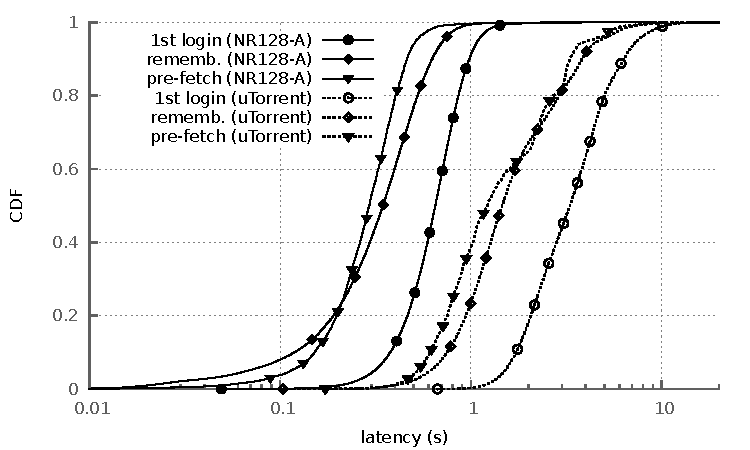
\includegraphics[width=.48\textwidth]{images/passwords-peer-to-peer/latencyCDF}
% 	\figlabel{latencyNr128aCDF}
% }
% \subfigure[$\mu$Torrent times]{
% 	\includegraphics[width=.48\textwidth]{images/passwords-peer-to-peer/latencyuTorrentCDF}
%   \figlabel{latencyuTorrentCDF}
% }
%   \caption{CDF for login latency in the three modes: First time login,
% remembered credentials, and first time login after password entry. Network
% operations assumed to have costs of BitTorrent mainline DHT lookup
% operations using NR128-A or $\mu$Torrent strategy~\cite{JimenezOK11}.} 
% \end{figure*}

\begin{figure}
 \centering
 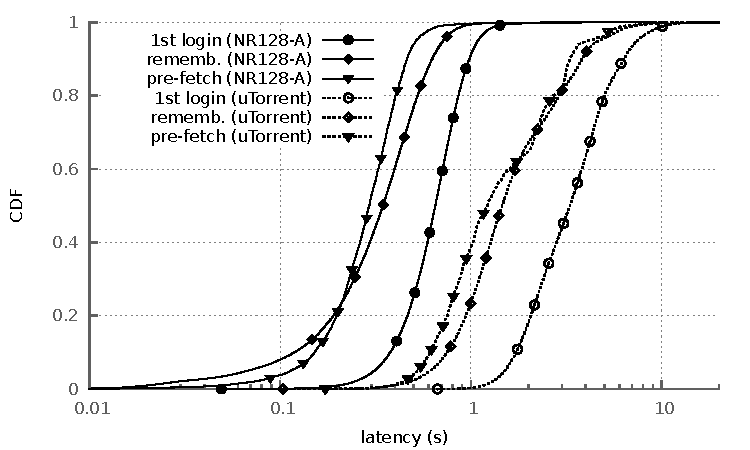
\includegraphics[width=.487\textwidth]{images/passwords-peer-to-peer/latencyCDF}
 \caption{CDF for login latency in three modes: First time login,
remembered logins, and first time login after password entry (pre-fetch). Network 
operations are assumed to have costs of BitTorrent mainline DHT lookups,
using NR128-A (solid lines) or $\mu$Torrent strategy (dashed lines)~\cite{JimenezOK11}.} 
 \figlabel{latencyCDF}
\end{figure}

We believe that the main performance-critical operation is logging
in~\cite{Rushinek86}. We believe that for all other operations,
latency on the order of a few seconds can be acceptable, and even a minute if they are run in the background. Thus, we only present results for logging in, but note
that as the operations for other protocols are similar, results are
expected to be similar. The performance cost of our protocols is
dominated by network operations. However, to slow down password
guessing attempts, one may wish to force the key derivation procedure
to be slow, to the point of making that cost dominant.

When evaluating the protocols, we parallelized network operations where
possible. Logging in for the first time and remembering the credentials for
future logins is then a sequence of two network operations, followed by key
derivation, followed by three parallel network operations. In a password
login, it is also possible to pre-fetch some of the information after the user
has entered her username, but before she enters her password. In
particular, as soon as the username is known, the filename $F_{LI}$ can be
retrieved from the DHT, and the file can be read. Decryption of the file and
further processing is then only possible after the user enters her password.
To evaluate % the gains of 
this speed-up, we computed the time it takes to
finish the login after the user has entered her password. The time to fetch
the two files is identical to the time to do a remembered login, and it is
sufficiently small that the data can realistically be retrieved while the user
is typing her password.

\begin{table}
\caption{Latencies of protocols, in milliseconds.}
\tablabel{latencies}
\centering
\newcommand{\mc}[3]{\multicolumn{#1}{#2}{#3}}
\begin{tabular}{lcccccc}
% 	\toprule
    & \mc{2}{c}{Network Op.~\cite{JimenezOK11}} & \mc{2}{c}{First Login} & \mc{2}{c}{Remem.\ Login}\\
	\cmidrule{2-7}
	DHT & median & $99^{\mathrm{th}}$  & median & $99^{\mathrm{th}}$  & median & $99^{\mathrm{th}}$  \\
	\midrule
	NR128-A & 164 & 567 & 650 & 1362 & 346 & 915 \\
	$\mu$Torrent & 647 & 5140 & 3299 & 10154 & 1456 & 7148 \\
	\bottomrule
\end{tabular}
\end{table}

To determine the sensitivity of our performance to implementation
characteristics, we evaluated our protocol for two different client strategies 
in the BitTorrent Mainline DHT:
The NR128-A algorithm~\cite{JimenezOK11}, and the
$\mu$Torrent client's implementation. We present these performance numbers in
\figref{latencyCDF} and 
\tabref{latencies}. Firstly, we observe that with a fast storage, our login
protocol is very fast, with a median login time of 650\,ms the first time, and
346\,ms for remembered logins. Comparing the results, we
observe that our protocols are indeed sensitive to storage latency. While
performance results building on $\mu$Torrent data are slightly above recommended
levels \cite{ToliaAS06}, we still consider them within range of acceptability
for P2P.

When evaluating these numbers, we assumed that the run-time of the KDF
function is negligible. As a system designer, one may wish to pick a slow KDF
(\eg bcrypt~\cite{DBLP:conf/usenix/ProvosM99}), as this slows down
password guessing attempts. Any latency intentionally added via the KDF would
affect the first-time login (after the password entry) times.


\subsection{Parameters for E-mail Password Recovery} \seclabel{evalemail}

%\begin{figure}
%  \centering
%	\includegraphics[width=.45\textwidth]{images/passwords-peer-to-peer/fixedn}
%  \caption{E-mail recovery: availability (probability of an immediately 
%successful password recovery) vs. security (success probability of an
%attacker, controlling 10\% or 25\% of the nodes) 
%for different $k$ ($n = 12$).}
%  \figlabel{fixedn}
%\end{figure}

%\begin{figure}
%  \centering
%	\includegraphics[width=.45\textwidth]{images/passwords-peer-to-peer/fixedk}
%  \caption{E-mail recovery: availability vs. security for different $n$ ($k$ = $n/2$)}
%  \figlabel{fixedk}
%\end{figure}

%\item Explain that there is a trade-off between three parameters (outlined
%below): availability, attacker success rate, and storage space
There are trade-offs between availability, security, and storage space in our e-mail based password recovery protocol.

%Describe the selection of $k$ parameter for a fixed $n$, a trade-off
%between availability and attacker success rate (\figref{fixedn})
For the selection of $k$, the minimum number of peers required to
recover the password, there is a direct trade-off between security and
availability.  Lower choices of $k$ increase the risk of an adversary,
controlling a significant number of nodes, to break into the user's
account. A higher $k$ reduces the availability of the recovery
functionality, which reflects the chances of a user to immediately
succeed with the password recovery.  However, if the user does not
instantly receive $k$ answers, she can simply wait until enough peers
are online.


We believe a reasonable choice of parameters is $n = 16$ and $k = n/2$. With
these numbers, using the availability data from Rzadca\etal~\cite{RzadcaDB10},
there is a 96\% probability of immediate recovery of a lost password. A very
strong attacker, corrupting 25\% of the nodes in the system, would still only
be able to access the user's account with probability 3\%.  The analysis of
parameter choice here is similar to any P2P system using secret sharing, and
we refer to e.g., Vu\etal \cite{Vu_Aberer_Buchegger_Datta_2009} for a more
in-depth discussion.

\subsection{Scalability}

The latency of our protocols will scale similarly to DHTs or other distributed
storage systems. The data we used for evaluation is based on measurements on
the largest deployed DHT, demonstrating that performance is good with
extremely large user numbers. Performance may in fact be worse for a small
system, as there are then fewer nodes, meaning that it is less likely to find
data at a nearby node. To bootstrap the system with good performance when it
is small, a very simple distributed storage using one or a few super-nodes
would be one approach. Storage requirements per user are also small, with a
few files per user and small file sizes. From this, we conclude that our
system is likely to scale well with the number of users.

\section{Conclusions and Future Work} \seclabel{conclusions}

The pros and cons of password-based authentication have been extensively
debated. We believe that for some applications, a username-password pair
provides an appropriate level of security. We argue that incorporating a
well-known authentication scheme may assist in user adoption of P2P systems
for more complex tasks than file sharing. To the best of our knowledge, ours
is the first work to focus on password-based logins in a P2P setting,
including mechanisms to recover a forgotten password. Our protocols are new
(but our security questions are similar to~\cite{FrykholmJ01}), relatively
straightforward, and we believe, they are an important first step towards
usable authentication in P2P. 

The performance of our mechanisms in terms of delay varies according
to the underlying DHT or P2P system in general and in relation to how
much intentional delay is added by parameterizing cryptographic
functions. Overall, however, our evaluation results show that for user
satisfaction~\cite{Rushinek86}, the delays can be kept at a very
acceptable level~\cite{ToliaAS06}.

While we have provided an initial discussion of the
security properties of our protocol here, future work will include a thorough
security analysis. Our scheme allows offline password guessing attacks, which
will also be addressed in future work.

\section*{Acknowledgments}

We thank Raúl Jiménez\etal{} %and his co-authors of
\cite{JimenezOK11} for sharing their measurement results and Jay Lorch for
excellent work as a shepherd of this paper. This research has been funded by
the Swedish Foundation for Strategic Research grant SSF FFL09-0086 and the
Swedish Research Council grant VR 2009-3793.


% last page column balancing (break column after specified bib entry)
%\IEEEtriggeratref{7}


% \bibliographystyle{IEEEtran}
% \bibliography{p2plogin}

% \end{document}

\acresetall
\chapter{\usebibentry{RodriguezCanoG14}{title}}
    \label[artsec]{article:thesis:events-invitations-dosns}
% -*- mode: TeX -*-
% -*- coding: utf-8 -*-

%%%%%%%%%%%%%%%%%%%%%%% file typeinst.tex %%%%%%%%%%%%%%%%%%%%%%%%%

% This is the LaTeX source for the instructions to authors using
% the LaTeX document class 'llncs.cls' for contributions to
% the Lecture Notes in Computer Sciences series.
% http://www.springer.com/lncs       Springer Heidelberg 2006/05/04
%
% It may be used as a template for your own input - copy it
% to a new file with a new name and use it as the basis
% for your article.
%
% NB: the document class 'llncs' has its own and detailed documentation, see
% ftp://ftp.springer.de/data/pubftp/pub/tex/latex/llncs/latex2e/llncsdoc.pdf
%
%%%%%%%%%%%%%%%%%%%%%%%%%%%%%%%%%%%%%%%%%%%%%%%%%%%%%%%%%%%%%%%%%%%

% \RequirePackage[l2tabu, orthodox]{nag}
% \documentclass[runningheads,a4paper]{utils/llncs}

% *** packages ***
% \usepackage{enumitem}
% \usepackage{bold-extra}
% \usepackage{amssymb}
% \usepackage{amsmath}
% \usepackage{amsfonts}
% \usepackage{bm}
% \usepackage{breqn}
% \setcounter{tocdepth}{3}
% \usepackage[pdftex]{graphicx}
% \usepackage{url}
% \usepackage{acro}
% \usepackage{glossaries}
% \usepackage{mfirstuc}
% \usepackage{xparse}
% \usepackage{booktabs}
% \usepackage{multirow}
% \usepackage{array}
% \usepackage{colortbl}
% \usepackage{arydshln}
% \usepackage{tikz}
% \usepackage{mdframed}
% \usepackage{cleveref}
% \usepackage{calc}
% %\usepackage{todo}
% %\usepackage{cite}
% %\usepackage[numbers]{natbib}


% *** fixed column sizes  ***
% \newcolumntype{L}[1]{>{\raggedright\let\newline\\\arraybackslash\hspace{0pt}}m{#1}}
% \newcolumntype{C}[1]{>{\centering\let\newline\\\arraybackslash\hspace{0pt}}m{#1}}
% \newcolumntype{R}[1]{>{\raggedleft\let\newline\\\arraybackslash\hspace{0pt}}m{#1}}

% % *** proper circled letters command ****
% \newcommand*\circled[1]{
%     \tikz[baseline=(char.base)]{\node[shape=circle,draw,inner sep=1.5pt] (char) {#1};}}
%
% % *** properties' frame command ***
% \newenvironment{propertydef}[1][]{%
%     \mdfsetup{%
%         frametitle={%
%             \tikz[baseline]=(current bounding box.east),outer sep=0pt]
%             \node[anchor=east,rectangle,fill=black!15]
%             {\strut #1};
%         },%
%         skipabove=1em,%
% %        skipbelow=1em,%
%         innerrightmargin=0pt,%
%         linecolor=black,%
%         linewidth=1.5pt,%
%         topline=false,%
%         bottomline=false,%
%         leftline=true,%
%         rightline=false,%
%         frametitleaboveskip=\dimexpr-\ht\strutbox\relax%
%     }
%
% \begin{mdframed}[]\relax%
% }{\end{mdframed}}

% *** images' settings ***
% \graphicspath{{./images/}}
% \DeclareGraphicsExtensions{.pdf,.jpeg,.png}

% \urldef{\mailsa}\path|{gurc, bgre, buc}@csc.kth.se|
% \newcommand{\keywords}[1]{\par\addvspace\baselineskip
% \noindent\keywordname\enspace\ignorespaces#1}

% *** capitalisation config for acronyms ***
% \acsetup{uc-cmd=\capitalisewords}

% *** definitions ***
% \newcommand{\etal}{ et\,al. }
% \newcommand{\eg}{e.\,g.,\ } % note the trailing comma (recommended by http://grammar.quickanddirtytips.com/ie-eg-oh-my.aspx )
% \newcommand{\Eg}{E.\,g.,\ }
% \newcommand{\ie}{i.\,e.,\ }
% \newcommand{\Ie}{I.\,e.,\ }

% \begin{document}

% \mainmatter  % start of an individual contribution

% first the title is needed
% %\title{Event Invitations in Privacy-Preserving \Aclp*{dosn}}
% \title{Event Invitations in Privacy-Preserving \acsp*{dosn}}
% %\subtitle{Formalization and Design of Protocols}
% %\subtitle{Formalization and Protocols Design}
% \subtitle{Formalization and Protocol Design}

% a short form should be given in case it is too long for the running head
% \titlerunning{Event Invitations in Privacy-Preserving \acsp*{dosn}}
%\titlerunning{Event Invitations in Privacy-Preserving Decentralized \acsp*{osn}}



% the name(s) of the author(s) follow(s) next
%
% NB: Chinese authors should write their first names(s) in front of
% their surnames. This ensures that the names appear correctly in
% the running heads and the author index.
%
% \author{Guillermo Rodr\'{i}guez-Cano \and Benjamin Greschbach \and Sonja Buchegger}
%
% \authorrunning{Guillermo Rodr\'{i}guez-Cano \and Benjamin Greschbach \and Sonja Buchegger}
% (feature abused for this document to repeat the title also on left hand pages)

% the affiliations are given next; don't give your e-mail address
% unless you accept that it will be published
% \institute{KTH Royal Institute of Technology\\
% School of Computer Science and Communication\\
% Stockholm, Sweden\\
% \mailsa}

%
% NB: a more complex sample for affiliations and the mapping to the
% corresponding authors can be found in the file "llncs.dem"
% (search for the string "\mainmatter" where a contribution starts).
% "llncs.dem" accompanies the document class "llncs.cls".
%

% \maketitle
\begin{center}
Guillermo Rodr\'{i}guez-Cano, Benjamin Greschbach, and Sonja Buchegger\\[2em]

KTH Royal Institute of Technology\\
School of Computer Science and Communication\\
Stockholm, Sweden\\
% \{gurc, bgre, buc\}@csc.kth.se
\{\href{gurc@csc.kth.se}{gurc}, \href{bgre@csc.kth.se}{bgre}, \href{buc@csc.kth.se}{buc}\}@csc.kth.se
\end{center}



% *** commands ***
\DeclareDocumentCommand{\e}{ O{k} }{\ensuremath{e_#1}} % event identifier = event public key
\DeclareDocumentCommand{\eS}{ O{k} }{\ensuremath{e_#1^S}} % event identifier = event private key
\DeclareDocumentCommand{\eo}{ O{k} }{\ensuremath{event_#1}} % event object = container of several information objects (event identifier, ...)
\DeclareDocumentCommand{\dP}{ O{k} }{\ensuremath{d_{\e[#1]}}} % public event description
\DeclareDocumentCommand{\dS}{ O{k} }{\ensuremath{d_{\e[#1]}^S}} % private event description
\DeclareDocumentCommand{\PDK}{ }{\ensuremath{PDK}} % encryption key for \dS
%\DeclareDocumentCommand{\IL}{ }{\ensuremath{IL}} % invite-list 
\DeclareDocumentCommand{\ILL}{ }{\ensuremath{ILL}} % invite-list link 
\DeclareDocumentCommand{\ILK}{ }{\ensuremath{ILK}} % invite-list encryption key 
%\DeclareDocumentCommand{\CL}{ }{\ensuremath{CL}} % commit-list
\DeclareDocumentCommand{\CLL}{ }{\ensuremath{CLL}} % commit-list link
%\DeclareDocumentCommand{\DL}{ }{\ensuremath{DL}} % disclose-list
\DeclareDocumentCommand{\DLL}{ }{\ensuremath{DLL}} % disclose-list link
\DeclareDocumentCommand{\u}{ O{j} }{\ensuremath{u_#1}} % user identifier = user public key
\DeclareDocumentCommand{\uS}{ O{j} }{\ensuremath{u_#1^S}} % user identifier = user private key
\DeclareDocumentCommand{\o}{ O{k} }{\ensuremath{o_{\e[#1]}}} % organizing user = organizer 
\DeclareDocumentCommand{\i}{ O{k} O{j} }{\ensuremath{i_{\e[#1]}^{\u[#2]}}} % invitation object
\DeclareDocumentCommand{\cm}{ O{k} O{j} }{\ensuremath{c_{\e[#1]}^{\u[#2]}}} % commitment object

\DeclareDocumentCommand{\U}{ }{\ensuremath{U}} % users
\DeclareDocumentCommand{\I}{ O{k} }{\ensuremath{I_{\e[#1]}}} % invitees
\DeclareDocumentCommand{\C}{ O{k} }{\ensuremath{C_{\e[#1]}}} % attendees
\DeclareDocumentCommand{\O}{ O{k} }{\ensuremath{O_{\e[#1]}}} % organizers

\DeclareDocumentCommand{\H}{ }{\ensuremath{H}} % hash function

\begin{abstract}
% 5 questions:
%
% What is the problem:
% Why is it a problem: 
% Why should we care: 
% What is our approach: 
% What are the findings: 

\Acp*{osn} have an infamous history of privacy and security issues. One approach 
to avoid the massive collection of sensitive data of all users at a central point 
is a decentralized architecture.

An event invitation feature -- allowing a user to create an event
and invite other users who then can confirm their attendance --
is part of the standard functionality of \acsp*{osn}. 
%
We formalize security and privacy properties of such a feature 
like allowing different types
of information related to the event (\eg how many people are
invited/attending, who is invited/attending) to be shared with 
different groups of users (\eg only invited/attending users).
%or only attending users to see an additional private event description.

Implementing this 
feature in a Privacy-Preserving \Acl*{dosn} is non-trivial because there is 
no fully trusted broker to guarantee fairness to all parties involved. 
%
We propose a secure decentralized protocol for implementing
this feature, 
using tools such as storage location indirection, ciphertext inferences
and a disclose-secret-if-committed mechanism, derived from standard
cryptographic primitives.

The results can be applied in the context of Privacy-Preserving \acsp*{dosn}, but 
might also be useful in other domains that need mechanisms for cooperation and coordination, 
\eg \Acl*{cwe} and the corresponding collaborative-specific tools, \ie groupware, 
or \Acl*{cscl}.

%\keywords{Event Invitation, Privacy, \Aclp*{dosn}}
% \begin{center}
%     Event Invitation, Privacy, \Aclp*{dosn}
% \end{center}
\end{abstract}

\clearpage
\section{Introduction}
	\label{section:event-invitations-dosns:introduction}
The most common form of \Acp{osn} are run in a logically centralized manner (although 
often physically distributed), where the provider operating the service acts as 
a communication channel between the individuals. 
Due to the popularity of these services, the extent of information 
the providers oversee is vast and covers a large portion of the population. 
Moreover, the collection of new types of sensitive information from each individual 
simply keeps increasing \cite{Smith2014}.
%
Users of these centralized services not only risk their own privacy 
but also the privacy of those they engage with. 
Whether intentional, or unintentional, data leakages \cite{Shih2013}, 
misuse \cite{Lunden2012} or censorship are some of 
the issues affecting the users. 

Decentralization has been proposed to reduce the effect of these privacy threats
by removing the central provider and its ability to collect and 
mine the data uploaded by the users as well as behavioral data. A \Ac{dosn} should 
provide the same features as those offered in centralized \Acp{osn} and 
at the same time it must preserve the privacy of the user in this different 
scenario. The latter is not straightforward, 
as in addition to the decentralization challenge itself, new privacy threats 
arise when the gatekeeper functionality of the provider that protects users from each other 
disappears \cite{GreschbachKB12}.

One of the standard features of \Acp{osn} is the handling 
of event invitations and participation, \ie a call for an assembly of individuals 
in the social graph for a particular purpose, \eg a birthday celebration, demonstration, 
or meeting. There is usually metadata related to each event, such as date, 
location and a description.
An implementation of this feature must provide security properties to the participants, \eg
that a user can verify that an invitation she received was actually sent
by the organizer. Furthermore, it must support certain privacy settings.
For example, an organizer could choose that only invited users learn how
many other users were invited and that only after a user has committed
to attend the event, she learns the identities of these other invited
users.

Realizing this in a decentralized scenario is non-trivial because there
is no \Ac{ttp} which all involved users can rely on. This is a problem, 
especially for privacy properties where information shall only be
disclosed to users with a certain status, because any user should be able 
to verify the results to detect any possible cheating. In the example above, a
neutral, trusted broker could keep the secret information (the
identities of invited users) and disclose it only to users who
committed to attend the event. This would guarantee fairness to both the
organizer and the invited users. It becomes more challenging to
implement this without a central \Ac{ttp} and still allowing different
types of information about the event to be shared with different groups
of users in a secure way.

\subsection{Our contribution}
	\label{subsection:event-invitations-dosns:our-contribution}
We describe and formally define two basic and five more complex security
and privacy properties for the event invitations feature. 

We propose and discuss a distributed and privacy-preserving implementation
of the event invitations feature without using a \Ac{ttp}. The
suggested protocols cover all of our defined properties, considering 20
different parameter combinations for the tunable privacy properties.

We also describe three privacy-enhancing tools that we use in our
implementation: storage location indirection, controlled ciphertext
inference and a \acl*{cdp}.
They are based on
standard cryptographic techniques such 
as public key encryption, digital signatures and cryptographic hashes,
and can be useful for other applications 
as well.

\subsection{Paper Outline}
	\label{subsection:event-invitations-dosns:paper-outline}
We discuss related work in \Cref{section:event-invitations-dosns:related-work}, describe the problem of implementing the event invitation 
feature in a decentralized way and formalize security and privacy properties in \Cref{section:event-invitations-dosns:decentralizing-the-event-invitation-feature}. 
Our proposed implementation together with privacy-enhancing tools follow in \Cref{section:event-invitations-dosns:implementation}, and we discuss 
this solution in \Cref{section:event-invitations-dosns:discussion}. 
We conclude with a summary and future work in \Cref{section:event-invitations-dosns:conclusion-and-future-work}.

\section{Related work}
	\label{section:event-invitations-dosns:related-work}
Groupware tools have been widely researched since they were first defined in 1978 
by Peter and Trudy Johnson-Lenz \cite{JohnsonLenz98}. 
%
Choosing between centralized and distributed implementations has been a major concern 
for these applications as pointed out in \cite{ReinhardSVW94}. While the traditional
model uses the client-server architecture \cite{TrevorKW97,LiOFWLN04}, there have 
been some projects on decentralized collaborative environments: \Acl{pecole} \cite{El-SaddikRAS08}, 
a \acs*{p2p} multicast overlay for multimedia collaboration in real-time, although 
synchronous; \acs*{ycab} \cite{BuszkoLH01}, a mobile collaborative system designed 
for wireless ad-hoc networks; or a hybrid \acs*{p2p} architecture with centralized 
personal and group media tools in \cite{ZhangJ06}.

Security features in collaborative applications were already introduced in the popular 
client-server platform for businesses, \acs*{ibm} Notes/Domino (formerly Lotus Notes/Domino), 
to allow for usable authentication, and digital signature and encryption by means 
of a \Ac{pki} to end-users \cite{Zurko05}. Control policies in \Ac{cscw} are considered 
in \cite{RoddenB91}, including distributed architectures.
%in \cite{RoddenB91}, in particular for distributed architectures, the authors believe 
%that the semantics of the cooperation should be reflected in the access rules.

Protocol design guidelines in collaboration scenarios, where the privacy 
of a group member does not lessen by participating in the 
environment, have been studied and proposed in \cite{KimK06a}. These guidelines aim 
at minimizing the amount of information a member has to provide to the group for 
the common activities, and making the protocols and 
the tasks transparent to everyone in the group.
%\cite{XhafaP10}

Another type of related work lies within the domain of \Acp{dosn} \cite{BadenBSBS09,CutilloMS09,FamulariH12}. To the best of 
our knowledge the event invitations feature has not been investigated in a privacy-preserving 
manner in this decentralized scenario.

\section{Decentralizing The Event Invitation Feature}
	\label{section:event-invitations-dosns:decentralizing-the-event-invitation-feature}

We already described the intuition of   
an event, where a group of people gathers with the intention of carrying 
out some activity. Now we more formally model the event invitation
feature and desirable security and privacy properties. 
%
We denote the set of users as $\U{} = u_1, \dots, u_n$. 
The event invitation happens in three main stages: 

\begin{itemize}
	
	\item \textbf{Creation:}
		When a user $\u[i] \in \U{}$ decides to create a new event \e{}, she becomes 
		the organizer \o{} and creates the event object \eo{} including different 
		information, \eg a description, date, time and location.
	
	\item \textbf{Invitation:}
		The organizer \o{} selects the set of users to be invited to the event \e{}, 
		denoted by \I{}, crafts the invitation objects \i{} for each of these invitees, 
		and sends them to the respective users. 
	
	\item \textbf{Commitment:}
		The invitees \I{} have the chance of confirming the invitation, \ie ``commit'' 
		to attend the event \e{}, by issuing commitment objects \cm{}. We denote 
		the set of all attendees, \ie the users who committed to the event \e{},
		as \C{}.
	
\end{itemize}

\Cref{figure:event-invitations-dosns:system-overview} shows an example with eight users, $\u[1] \dots \u[8]$, where one 
of them, \u[1], is the responsible organizer \o{} of the event \e{}. 
The organizer issues invitations to $\u[2] \dots \u[6]$, depicted with 
a dashed line. These users form the group of invitees, denoted with \I.
Invited users who confirm their attendance, (\u[2], \u[4] and \u[6] in
this example), provide a commitment to the organizer, depicted with a
continuous line. They form the group of attendees, denoted with \C.

\begin{figure}
  \centering
  \includegraphics[width=.73\linewidth]{images/event-invitations-dosns/system-overview}
  \caption{Example of one event invitation.}
  \label{figure:event-invitations-dosns:system-overview}
\end{figure}

A possible privacy setting
could specify that invited users learn how many other users are invited
but only attending users learn their identities. That is, $\u[3]$
and $\u[5]$ would learn that five users are invited (while this is kept
secret from $\u[7]$ and $\u[8]$). $\u[2], \u[4]$ and $\u[6]$
would additionally learn the identities of $\I = \u[2] \dots \u[6]$.

\subsection{System Model and Assumptions}
	\label{subsection:event-invitations-dosns:system-model-and-assumptions}
In the following, we
assume basic functionalities of popular \Acp{osn} to be available in 
a decentralized manner, such as user 
search \cite{GreschbachKB2013} and user messaging \cite{RowstronD2001}.
%
We also assume that users are identified by a public key and the ability  
to verify the identity of other users via some sort of \Ac{pki}, which can 
be realized in a decentralized manner, \eg a ``Web of Trust'' model or a Bitcoin 
block-chain binding friendly usernames to public keys \cite{Freitas2013}. 
%
Moreover, we rely on a distributed storage
featuring access right management, \eg that a certain storage object is
only writeable by a specific user, and ``append-only'' storage objects,
where new data can be appended, but existing data cannot be modified or
removed without notice. The latter can be realized in a decentralized
fashion, \eg in a similar manner as the Bitcoin block-chain is secured
against modifications \cite{Nakamoto08}. 
% implementation details: the link is a random serial-number and a pointer to the current blockchain head. Entries just repeat the serial-number (or even a salted hash of it? more costly but less linkable). The row number can be the block number (does not need to be consecutive, only strictly increasing). Disclose-list entries are distinguished by a flag. 


\subsection{Threat Model}
	\label{subsection:event-invitations-dosns:threat-model}

We assume that users in all roles, \eg invited users or
the organizer of an event, might act maliciously, \ie become
adversaries. The capabilities of an adversary range from passively
learning information accessible in that role (\eg an invited
user might have access to a list of all other invited users, depending
on the privacy settings for the event), to actively interacting with
other parties, \eg writing arbitrary data to accessible storage
objects or sending arbitrary messages to other users. We also assume
that powerful adversaries might have the possibility to pervasively
monitor a large fraction of the network traffic. While we try to
mitigate threats like traffic analysis and correlation attacks arising
from this, we cannot completely protect against
them and come back to this in the discussion section. We do not assume
that adversaries can subvert the storage layer. So we
assume the availability of a secure distributed storage including
features like append-only lists and authorization mechanisms, as
mentioned above. % Furthermore, we rely on a secure PKI, so no impersonation, ...

We want to keep malicious users from undermining the reliability of the
event invitation feature for legitimate users. This means that an
adversary should not be able to violate the security and privacy
properties that we define in the next section. 
This comprises guaranteeing the authenticity and non-repudiation of
statements made by the involved parties, such as issued invitations or
commitments. 
Furthermore it includes keeping information such as the identities of
invited/attending users, the number of invited/attending users or a
private event description secret from unauthorized users while
guaranteeing its availability and authenticity for legitimate users.
An example for the latter would be to keep an organizer 
from withholding or lying about the number of attending users.
%
We do not focus on denial-of-service attacks and leave
them for future work.

\subsection{Security and Privacy Properties}
	\label{subsection:event-invitations-dosns:security-properties}
A protocol for event invitations can comply with different security and
privacy properties. We first list the following basic security properties:

\begin{itemize}
	
	\item \textit{A user \u{} can prove that she was invited to the
					event \e{} if and only if the organizer
					\o{} invited \u{}, \ie issued an
					invitation \i{}.} 

	This property is two-sided and guarantees that a user cannot forge
	an invitation she did not get, while an organizer cannot deny that
	she invited a user. 
	This implies that an invitation \i{} is tied to a user \u{} that was
	chosen by the organizer \o{} and cannot be transferred to another user.\\

	
	\item \textit{An organizer \o{} can prove that the invited 
		user \u{} committed to attend the event \e{} if and only if \u{}
		actually committed, \ie issued a commitment \cm{}.}

	This property also has two sides. The organizer cannot forge a commitment
	of a user that did not commit to the event. And a user cannot deny
	that she committed to an event once she did so.

\end{itemize}

\noindent More challenging properties are those defining which groups of
users are allowed to see what information, namely, 

{
	\setlength{\parskip}{.5em}
	
	% who sees who else is invited
	\begin{propertydef}[\Ac{iip}]
		\textit{For an event \e{}, only a chosen 
		set of users (\eg \U{}, \I{}, \C{} or only \o{}) learns
		who else is invited (\ie sees all members of \I{})}.
		\par \noindent
		This property defines who can see information about who is invited to
		an event. 
		This can be all users (\U{}) or be restricted so that only other
		invited users see who else is invited (\I{}). Another
		possibility is that even an invited user first learns who else is
		invited when she committed to attend (\C{}). Finally, this
		information could be kept completely secret, so only the organizer \o{}
	    knows the complete list of invited users.
	\end{propertydef}
	
	% who sees how many are invited
	\begin{propertydef}[\Ac{icp}]
		\textit{For an event \e{}, only a chosen 
		set of users (\eg \U{}, \I{}, \C{} or only \o{}) learns
		how many users are invited (\ie learns $| \I{} |$)}.
		\par \noindent
		This property is a variant of property \Ac{iip} where the number of
		the invited people \I{} is disclosed to a set of users (while
		the identities of the invited people might remain hidden).
	\end{propertydef}
	Property \Ac{iip} and \Ac{icp} are closely related in the sense that if \Ac{iip}
	holds for a certain set of users, then \Ac{icp} trivially holds for
	the same set (and all its subsets -- note the 
	subset relation of the possible sets to choose from, $\U{} \supseteq \I{} \supseteq \C{}$). 
	
	\noindent This constrains the possible combinations 
	of these two properties' parameters. If, for example, for a certain event all 
	invited users \I{} should see who else was invited, \ie property \Ac{iip} with parameter 
	choice \I{}, then it does not make sense to choose that only the attendees \C{} should 
	learn the number of invited people, \ie property \Ac{icp} with parameter choice 
	\C{}, because the invited users can already derive this information from what 
	they learn from property \Ac{iip}.

	% who sees who else has committed
	\begin{propertydef}[\Ac{aip}]
		\textit{For an event \e{}, only a chosen
		set of users (\eg \U{}, \I{}, \C{} or only \o{}) learns
		who is attending (\ie sees all members of \C{})}.
	\end{propertydef}

	% who sees how many have committed
	\begin{propertydef}[\Ac{acp}]
		\textit{For an event \e{}, only a chosen 
		set of users (\eg \U{}, \I{}, \C{} or only \o{}) learns
		how many users are attending (\ie learns $| \C{} |$)}.
	\end{propertydef}
	Similarly to properties \Ac{iip} and \Ac{icp}, these two properties specify who 
	can see information about the users who committed to attend an event.  
	Property \Ac{aip} defines who can see the identities of the attendees while 
	property \Ac{acp} defines to whom the number of attendees is disclosed. The 
	same relation, regarding the possible parameter choices, as
	described for properties \Ac{iip} and \Ac{icp}, also holds here.

	% organizer can claim "A coming"  iff  A can decrypt P
	% (i.e. Organizer cannot claim that A is coming if A cannot decrypt P,
	% and A cannot decrypt P if the organizer cannot claim that A is coming)
	\begin{propertydef}[\Ac{air}]
		\textit{An invited user \u{} can only get access to the private description 
		\dS{} of the event \e{} once committed and the organizer \o{} 
		can only claim the attendance of the user \u{} once the private description 
		\dS{} is available to \u{}}.
		\par \noindent
		This property has two sides. First, a user \u{} can only get access
		to information exclusive to the attendees \C{}, \ie the private description
		\dS{} from the organizer \o{} for an event \e{},
		if she has committed to attend. Second, and conversely, the
		organizer \o{} can only claim that user \u{} has
		committed to attend if she has made it possible for \u{} to access
		the private description \dS{}.
	\end{propertydef}

}

\section{Implementation}
	\label{section:event-invitations-dosns:implementation}
We now propose an implementation of the event invitation feature described in \Cref{section:event-invitations-dosns:decentralizing-the-event-invitation-feature} in 
a privacy-preserving \Ac{dosn}. We assume that user identifiers \u[i] are 
public keys, and we will denote their corresponding private keys as \uS[i] (where 
$S$ stands for ``secret'').

\subsection{System Components}
	\label{subsection:event-invitations-dosns:system-components}

The main components of the system are event objects, invitation objects
and commitment objects as depicted in \Cref{figure:event-invitations-dosns:overview-objects-actions}.

\begin{itemize}
%\paragraph{event object:}
\item \textbf{Event object:} 
When a user wants to create a new event, she first generates a
public/private keypair \e{}/\eS{}. The public key will become the 
identifier for the event and the user will be denoted as organizer \o{}. 
She then assembles the event object \eo{}: She writes a public
event description \dP{} and a private description \dS{} that
will be encrypted with a symmetric key \PDK{}. 
%
She creates one list to store the invitation objects (\emph{invite-list})
encrypted with a symmetric key \ILK{}, another list for the
commitment objects (\emph{commit-list}) and one for disclosing secret
information to committed users (\emph{disclose-list}). The event object
contains links \ILL{}, \CLL{} and \DLL{}, pointing to the storage
locations of these three lists.
%
Additionally the organizer creates a list of public/private keypairs
$rk_1/rk_1^S, \dots, rk_n/rk_n^S$, to encrypt the entries on the
commit-list, and includes the public keys in the event object.
%
Moreover, the event object contains information about the chosen privacy
settings. 

The organizer signs the public key of the event with her own user key to
confirm that she is the organizer and signs the whole event object
\eo{} with the event's private key \eS{}. Therefore, an event object is composed
as follows:
\begin{align*}
	\eo = Sign_{\eS{}}(& Sign_{u_i^S}(\e{})||u_i|| \dP || Enc_{\PDK}(\dS{}) \\
		&|| \ILL{} || \ILK{} || \CLL{} || \DLL{} || rk_1, \dots, rk_n || \text{privacy settings})
\end{align*}

Some of the elements of the event object might, however, be encrypted
with additional keys or only be hashes (made with a cryptographic hash
function \H{}, \eg SHA-2 \cite{GilbertH03}) of the actual values. This
depends on the chosen privacy settings and will be explained in more
detail later.
\\

\item \textbf{Invitation object:} 
%\paragraph{invitation object:}
An invitation object is composed of the invitee's identifier \u{} (her public 
key), signed by the organizer \o{} with the event's private key \eS{}:
\begin{equation*}
		\i{} = Sign_{\eS{}}(\u{})
\end{equation*}

\item \textbf{Commitment object:} 
%\paragraph{commitment object:}
A commitment object is composed of the invitation object \i{} and the cryptographic 
hash of the event object \eo{}, both signed by the attending 
user \u{} with her private key \uS{} as follows,
\begin{equation*}
		\cm{} = Sign_{\uS{}}(H(\eo{})||\i{})
\end{equation*}
\end{itemize}

\begin{figure}
  \centering
  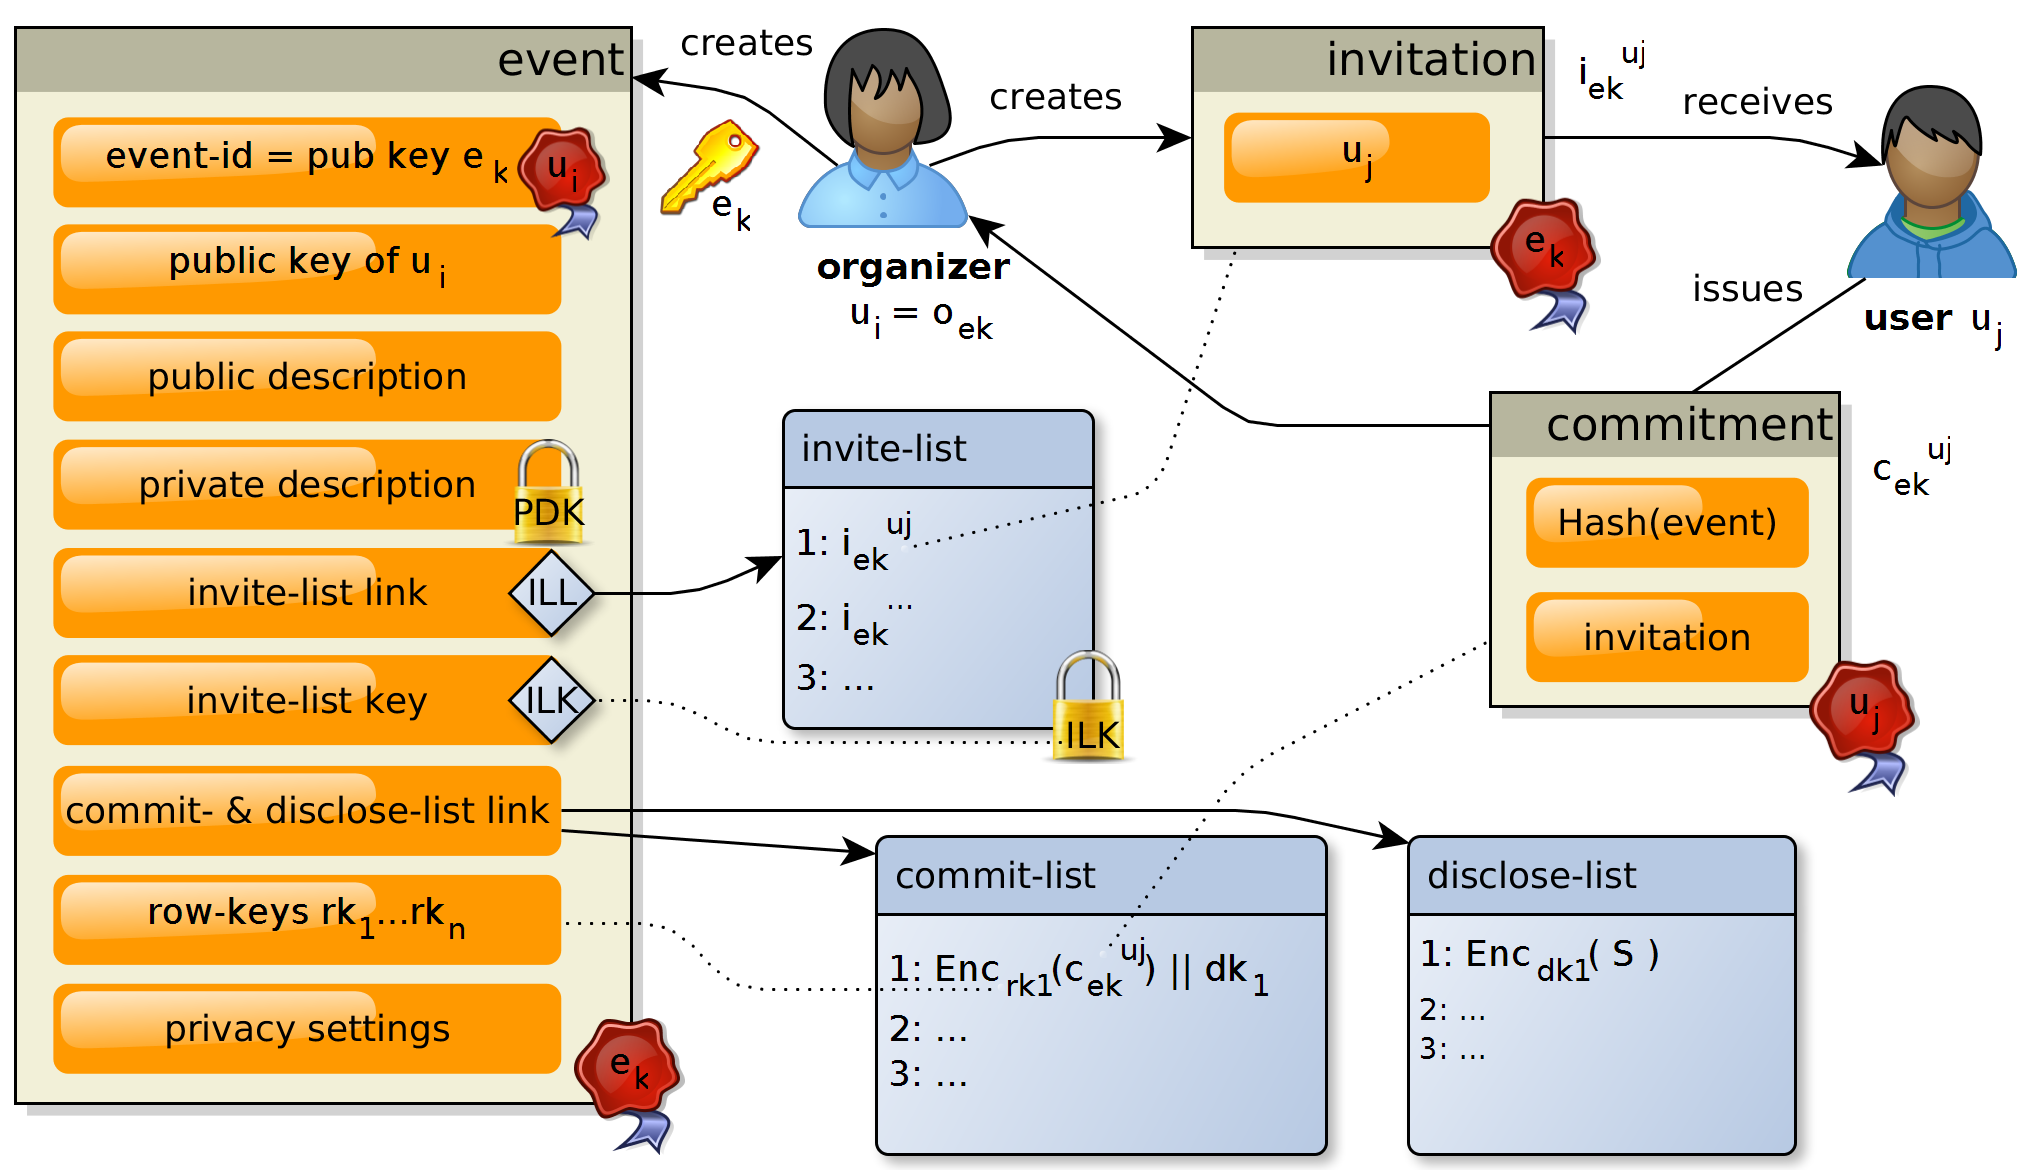
\includegraphics[width=.8\linewidth]{images/event-invitations-dosns/system-implementation}
  \caption{Overview of the actors, system components and their relations.}
  \label{figure:event-invitations-dosns:overview-objects-actions}
\end{figure}


\subsection{Privacy Enhancing Tools}
	\label{subsection:event-invitations-dosns:privacy-enhancing-tools}
Before describing the implementation, we introduce tools that we will use several times.

\subsubsection{Storage Location Indirection and Controlled Ciphertext Inference}
	\label{subsubsection:event-invitations-dosns:indirection-and-ciphertext-inferences}
If we want to make the size of a list, \ie the number of its elements, available 
to a subset of users, but not the content of 
the list elements (in our scenario because each element contains 
a user identifiers), we can use storage location indirection and ciphertext inference:
%
The list will not be stored together with the event object, but at a secret location in the distributed storage such that it can only 
be reached if the link to it is known. Additionally, the elements of the list will be encrypted so 
that the stored content can only be accessed if the encryption key is known. 

This provides the possibility of a controlled information disclosure depending on the knowledge of a user:
%
Users who do not know the link, learn nothing, neither the size nor the
content of the list.
%
Making the link to the list but not the encryption key available to 
a subset of users, enables these users to learn the size of the list
(assuming a constant ciphertext size for each entry), while
it does not give them any details about the contents stored.
%
Users that received both the link and the encryption key, learn the content 
and can act as verifiers, checking that there are no invalid entries 
that incorrectly increase the perceived number of elements as seen by
those users holding only the link but not the key. 

\subsubsection{Commit-Disclose Protocol}
	\label{subsubsection:event-invitations-dosns:commit-disclose-protocol}

The organizer may want to share some information only with users who
have committed to attend the event (attendees). To ensure 
fairness, the invited users need some guarantee that they can
expect to receive the promised information when they commit to attend.

While this is easy to solve if both parties, the organizer and the
invited users, trust a neutral third party that can act as broker, it
becomes more difficult in our setting where we do not assume the
existence of any \Ac{ttp}. So we base our solution on a significantly
weaker trust assumption: the availability of append-only storage objects
as described in \Cref{subsection:event-invitations-dosns:system-model-and-assumptions}. 

The aim of the protocol is to provide an invitee \u{} who commits to the event \e{} 
with a secret $S$ held by the organizer \o{}.  
It is composed of three main components, provided 
by the organizer of the event:

\begin{itemize}

	\item \textbf{Commit-List}, 
		a public and append-only storage object where invited users
		store their (encrypted) commitments.

	\item \textbf{Disclose-List},
		a public readable, but only writeable by the organizer,
		append-only storage object where the organizer discloses
		(encrypted) secrets for the committed users.

	\item \textbf{Anchor Point},
		a storage object (in our case the event object) serving as
		common entry point, referencing the commit-list and the
		disclose-list either directly by providing their storage
		locations, \ie a commit-list link \CLL{} and a disclose-list
		link \DLL{} or indirectly by holding salted hashes of these
		storage locations (where \DLL{} and \CLL{} together with the
		salts are shared with a subset of users in another way).
		Additionally, a list of public keys $rk_1, \dots, rk_n$, 
		called row-keys, used to encrypt the entries on the
		commit-list	are also stored here. 	
		All this information is signed by the organizer. % with the event's private key \eS{} that she holds.

\end{itemize}

\noindent Each key in the row-keys list is intended for encrypting one entry of the commit-list.
The corresponding private keys $rk_1^S, \dots, rk_n^S$, are held by the organizer.
%
The protocol runs in three phases:


\begin{itemize}
	\item \textbf{Commit Phase:}
		If the user \u{} wants to commit to attend the event \e{}, she
		looks up the commit-list and finds the next free row --
		let this have index $l$. She then looks up the corresponding row
		key $rk_l$ in the event object.
		
		Finally, she crafts a commitment \cm{}, creates a fresh keypair
		$dk_l^P/dk_l^S$ (disclose key, later used by the organizer to
		encrypt the secret information) and writes the following entry
		to row $l$ of the commit-list: $Enc_{rk_l}(\cm{}) || dk_l^P$
		that is the commitment, encrypted with the row-key, together
		with the public disclose key in plain.
		\\
	\item \textbf{Disclose Phase:}
		When the organizer \o{} sees that a new row $l$ has been added to the
		commit-list, she tries to decrypt the first entry, using the secret row
		key $rk_l^S$. If this succeeds and the commitment is valid % \ie contains a valid invitation, a correct hash of the event object and is signed by the right user key
		the organizer writes the secret information, encrypted with the provided 
		disclose key to row $l$ of the disclose-list, \ie $Enc_{dk_l^P}(S)$.
		If the decryption fails or the commitment is invalid, the
		organizer publishes the secret row-key of row $l$ in the
		disclose-list instead, \ie $rk_l^S$, 
		thus proving to everybody who can access the lists that she was not
		obliged to disclose the secret information to the creator of row $l$. % as now everybody can decrypt the first part of the commit-list entry in row $l$ and check that it did not contain a valid commitment
		\\
	\item \textbf{Blame Phase:}
		If the organizer misbehaves and does not provide a
		protocol-abiding user with the secret information after a
		reasonable amount of time, % can be realized with the bitcoin-blockchain style list implementation by defining a minimum number of blocks for the timeout
		the user can blame the organizer. She does this by publishing a
		blame-entry in the commit-list, referring to the row $l$ and
		disclosing the secret disclosure key $dk_l^S$. Thus everybody 
		who can access the lists can see that she did not receive the
		secret information encrypted to the disclosure key she provided
		in row $l$. It can be assumed that the commitment (which cannot be
		decrypted by the verifying public) was correct, as otherwise the
		organizer would have published the secret row-key of row $l$.
\end{itemize}

\noindent In this way, the \acl{cdp} does not keep the organizer
from cheating, but it allows the user to reliably blame the organizer % in front of a public of her choice (either all users who can access the lists, or even everybody if she publishes the links \CLL{} and \DLL{} (together with the salts) if they were not public
if it is the case.


\subsection{Basic Security Properties}
	\label{subsection:event-invitations-dosns:basic-security-properties}
The basic security properties are fulfilled by the construction of an event, invitations 
and commitments described in \Cref{subsection:event-invitations-dosns:system-components} and the guarantees 
of the \Ac{pki}. 
%
The first basic security property is fulfilled because an invitation \i{} for a user \u{} 
is created by using the event's private key \eS{}, owned by the organizer \o{} to 
sign the invited user's identifier. The invitee cannot forge the event's key and 
the organizer cannot deny having issued the invitation because 
the signature used to sign the invitation is publicly verifiable.
%
The second basic security property is also fulfilled because an organizer \o{} cannot forge 
a commitment \cm{} as she is not able to forge another users' signature. A %TODO?: replay attacks excluded becauese of having the hash of the event in the commitment
user \u{}, having sent the commitment \cm{} to the organizer \o{}, cannot deny the 
commitment as her signature is again publicly verifiable and binding to the event \e{}.

% \subsection{\Acl{iip} and \Acl{icp}}
\subsection{Invitee Identity Privacy and Invitee Count Privacy}
	\label{subsection:event-invitations-dosns:invitee-identity-and-count-privacy-properties}
In order to implement properties \Ac{iip} and \Ac{icp}, we let the organizer \o{} 
store all invitation objects for the event in the invite-list. 
Retrieving the list requires knowledge of the invite-list link \ILL{}, 
and in order to decrypt it, the symmetric invite-list key \ILK{} must be known 
beforehand.

Knowledge of the link \ILL{} is equivalent to learning the total number of invitations, 
even if the decryption key \ILK{} is unknown because the number of invitations can 
be inferred from the size of the ciphertext in the list.  
Knowledge of the encryption key \ILK{} allows learning the identities of the invited 
users \I{} because the invitations \i{} store the user identifiers in plain text.

If the organizer \o{} wants to make the identifiers of the invitees \I{}, or the 
amount of them, \ie $|\I{}|$, available to all users \U{}, she will publish 
\ILL{} or \ILK{} in plain text together with the event object \eo{}. Making this 
information available only for invitees \I{} can be realized
by the organizer privately sharing it with the invited users.
%
In order to share the decryption key \ILK{} only with the committed
users \C{}, the \acl{cdp} can be used, while the link \ILL{} 
is then either available publicly (\ie choosing \U{} for property \Ac{icp}), shared only 
with the invitees (\ie choosing \I{} for \Ac{icp}) or kept secret and only 
shared with the committed users together with \ILK{} (\ie choosing \C{} for 
\Ac{icp}). 

It is also possible to avoid sharing any information about the invitations by keeping 
\ILL{} and \ILK{} secret, \ie choosing \o{} both for properties \Ac{iip} and \Ac{icp}. 
When the identities should not be known to anyone but the number of invitees 
should be made public to a subset of users (\ie choosing \o{} for property \Ac{iip}), 
the link \ILL{} will be shared with the respective users and a particular encryption 
scheme for the invite-list is employed:
%
Instead of encrypting the invite-list as a whole, we encrypt its individual 
entries with the public keys of the recipient of the invitation stored at each entry. 
Thus, the invited users can verify that their own invitation is
included in the list. However, this only allows for a weak verification of the correctness 
of the list, \ie it provides an upper-bound of the size of the list, because the 
organizer \o{} can add invalid or dummy entries (\eg to artificially increase the 
perceived number of invitees to the event).

A summary of how \ILL{} and \ILK{} are shared depending on the choice of parameters 
for properties \Ac{iip} and \Ac{icp} is shown in \Cref{table:event-invitations-dosns:implementation-iip-icp}.
Note that the row describing the privacy settings \Ac{iip}: \C,
\Ac{icp}: \I corresponds to the example mentioned in the introduction
and \Cref{section:event-invitations-dosns:decentralizing-the-event-invitation-feature}.

\begin{table}
	
	\centering

	\caption{Sharing of \ILL{} and \ILK{} as per the \Ac{iip} and \Ac{icp} settings.
	P = publicly available in \eo{}, I = 
	privately shared with \I{}, C = shared only with \C{} (via the \acl{cdp}), S 
	= fully secret (only \o{} knows about it) and $\mathrm{S^*}$ = special encryption 
	scheme for the invite-list.}

	\begin{tabular}{@{\hspace{.5em}} c c c@{\hspace{.5em}} | c@{\hspace{.5em}} c c @{\hspace{.5em}}}
		\toprule
		\multicolumn{2}{c}{\textbf{\textsc{Settings}}} & & & \multicolumn{2}{c}{\textbf{\textsc{Implementation}}} \\
		\addlinespace[.3em]
		\textbf{\acs{iip}} & \textbf{\acs{icp}} & & & $\bm{\ILL{}}$ & $\bm{\ILK{}}$ \\
		\addlinespace[.1em]
		\midrule
		\U{}& \U{} & & & P & P \\
		\cdashline{1-6}[.4pt/1pt]
		\addlinespace[.3em]
		\multirow{2}{*}{\I{}} & \U{} & & & P & I \\
		& \I{} & & & I & I \\
		\cdashline{1-6}[.4pt/1pt]
		\addlinespace[.3em]
		\multirow{3}{*}{\C{}} & \U{} & & & P & C \\
		& \I{} & & & I & C \\
		& \C{} & & & C & C \\
		\cdashline{1-6}[.4pt/1pt]
		\addlinespace[.3em]
		\multirow{4}{*}{\o{}} & \U{} & & & P & $\mathrm{S^*}$ \\ 
		& \I{} & & & I & $\mathrm{S^*}$ \\
		& \C{} & & & C & $\mathrm{S^*}$ \\ 
		& \o{} & & & S & S \\
		\bottomrule
	\end{tabular}
	
	\label{table:event-invitations-dosns:implementation-iip-icp}
	
\end{table}


% \subsection{\Acl{aip} and \Acl{acp}}
\subsection{Attendee Identity Privacy and Attendee Count Privacy}
	\label{subsection:event-invitations-dosns:attendee-identity-and-count-privacy-properties}

To implement the \Ac{aip} and \Ac{acp} properties, we mainly use the \acl{cdp}.
%
The link to the commit-list \CLL{} can be shared publicly in the event object 
\eo{} except for those cases where the count of attendees $|\C{}|$ must be kept 
private. In this situation, if the invitees \I{} are allowed to learn $|\C{}|$, 
\CLL{} is shared privately with them. Alternatively, the organizer can add dummy entries 
in the list to hinder inferences from the number of (encrypted) entries. 
When not even attendees should learn how many other users are attending, 
dummy entries in the commit-list are the only solution as the \CLL{} must always 
be shared with all invitees, so that they can commit if they want to attend.

Dummy entries follow the pattern of usual entries, \ie random data with a specific 
size to fake an encrypted commitment object and a public key in the commit-list, and 
random data in the disclose-list to fake an encrypted secret. 
All users who hold the private row-keys can identify them 
because the first part of a dummy entry in the commit-list cannot be decrypted 
with the respective row-key, while those users without the private row-keys cannot distinguish 
dummy entries from real ones as the ciphertext structure looks the same for all 
of them. 

When the link \CLL{} should not be shared publicly in the event object \eo{}, a 
salted hash of the link will be stored instead so that the organizer 
\o{} cannot cheat by sharing different links with different groups of users. As the 
event object is unique per event and group of invitees, the invited
users can check they all got the same link % (together with a salt)
from the organizer by comparing it with the hash value in \eo{}.

Otherwise the implementation varies only in how the private row-keys are disclosed, 
as they protect the commitments in the commit-list: If all users 
\U{} are allowed to learn who is attending, the private row-keys will be public, \ie 
the rows do not need to be encrypted. If only the invited users \I{} should see 
the identities of the attendees, the private row-keys will be shared with the invitees 
directly. And if only the attending users should learn about the identities 
of other attendees, the private row-keys are disclosed using the \acl{cdp}.

This way we are able to implement all possible parameter combinations of
the \Ac{aip} and \Ac{acp} properties, except for the combination
\Ac{aip}: \o{}, \Ac{acp}: \C{}. For this case, \ie \Ac{aip}: \o{}, 
nobody except the organizer should learn the identities of the
committed users, so the private row-keys have to be kept secret. And as
not even invitees (who need to know \CLL{} to be able to commit to
the event) should learn the count of attendees, the organizer
would need to add dummy entries on the commit-list to hide the count of
attendees from the invitees. But this will also hide it from the
attendees, as they do not have the private row-keys to tell apart dummy
entries from normal entries, so \Ac{acp}: \C{} is not fulfilled.

A summary of how \CLL{} and the private row-keys $rk_1^S\dots rk_n^S$ are shared depending 
on the settings for properties \Ac{aip} and \Ac{acp} is shown in \Cref{table:event-invitations-dosns:implementation-aip-acp}.

\begin{table}
	
	\centering

	\caption{Sharing of \CLL{} and $rk_1^S\dots rk_n^S$ as per the \Ac{aip} and \Ac{acp} settings.
	P = publicly available in \eo{}, 
	I = privately shared with \I{}, C = shared only with \C{} (via the \acl{cdp} 
	), S = fully secret (only \o{} knows about it).}

	\begin{tabular}{@{\hspace{.5em}} c c c@{\hspace{.5em}} | c@{\hspace{.5em}} c c c c @{\hspace{.5em}}}
		\toprule
		\multicolumn{2}{c}{\textbf{\textsc{Settings}}} & & & \multicolumn{4}{c}{\textbf{\textsc{Implementation}}} \\
		\addlinespace[0.3em]
		\textbf{\acs{aip}} & \textbf{\acs{acp}} & & & $\bm{\CLL{}}$ & $\bm{rk}_1^S ... \bm{rk}_n^S$ & \textbf{dummies} & \textbf{notes} \\
		\addlinespace[0.1em]
		\midrule
		\U{} & \U{} & & & P & P & - & \\ % this is equal to having only the commit-list, without any encryption scheme or disclose keys on it 
		\cdashline{1-8}[.4pt/1pt]
		\addlinespace[0.3em]
		\multirow{2}{*}{\I{}} & \U{} & & & P & I & - & \\ 
		& \I{} & & & P/I & I & if CLL public & \\% if CLL not shared publicly, a (salted) hash must be published in the event object to ensure, that all invitees got the same link
		\cdashline{1-8}[.4pt/1pt]
		\addlinespace[0.3em]
		\multirow{3}{*}{\C{}} & \U{} & & & P & C & - & \\
		& \I{} & & & P/I & C & if CLL public & \\
		& \C{} & & & P & C & necessary & \\ % dummy entries necessary (we cannot hide the link, otherwise the protocol does not work)
		\cdashline{1-8}[.4pt/1pt]
		\addlinespace[0.3em]
		\multirow{4}{*}{\o{}} & \U{} & & & P & S & - & \\ 
		& \I{} & & & I & S & - & \\ % 
		& \C{} & & & - & - & - & not possible\\ % not possible 
		& \o{} & & & P & S & necessary & \\ % P to still enable Property 4
		\bottomrule
	\end{tabular}
	
	\label{table:event-invitations-dosns:implementation-aip-acp}
	
\end{table}

% implementatin details: the inference calculation from the size of the encrypted commit-list to 
% obtain the number of attending users must be modified, ignoring rows that are 
% outed as incorrect by the organizer via publishing the respective secret row 
% key in the disclose-list. (maybe no need to explain this as it is implicit)


% \subsection{\Acl{air} Property}
\subsection{Attendee-only Information Reliability Property}
	\label{subsection:event-invitations-dosns:air-property}
To implement this property, we will again use the \acl{cdp}. The 
organizer \o{} shares a private description \dS{}, encrypted with the key \PDK{}, 
with the committed users \C{}. The key is shared with these users in the
disclose-list as soon as they store a valid commitment \cm{} in the
commit-list.
%
The organizer \o{} cannot have different private descriptions for groups of attendees 
of the same event \e{} because they will all see the same ciphertext in the event 
object \eo{}.
%
A cheating organizer \o{} will be caught in the same manner as described 
above: if a user \u{} commits and receives an invalid decryption key \PDK{}, she 
will publish the private disclose key $dk_i^S$ to prove that she did not receive 
the promised private description \dS{}.


\section{Discussion}
	\label{section:event-invitations-dosns:discussion}

The implementation presented realizes the event invitation feature
in a decentralized system and fulfills the requirements of all of the
defined security and privacy properties. Except for one parameter
combination of the attendee identity/count privacy properties we were
able to present implementation solutions for all possible choices of the
tunable properties \Ac{iip}, \Ac{icp}, \Ac{aip} and \Ac{acp}.

An honest but curious user does not learn anything more than what is
specified by the privacy settings. 

A general limitation of our approach is, however, that for all
properties based on the \acl{cdp}, a malicious 
organizer is still able to cheat. But it disincentives her to do so as it
provides a reliable cheating detection mechanism and offers the affected
users the possibility to blame a cheating organizer -- either publicly
or in front of a chosen set of users, \eg only other invitees of the 
event. 
We consider this an effective protection in the social scenarios that we
see as possible application contexts of the event invitation feature.
User identifiers are long-lived there and costly to change (as all
friends have to be informed about a new identity), so we assume users 
care about their reputation and will try to avoid being exposed as
misbehaving.
%
% Write about cheating possibilities for organizer: why it will be
% detected if different secrets are shared with different users
%
% If the organizer withholds entries in the invite-list, she risks to
% be caught by those users when they commit.
% What if the organizer adds entries in the invite-list which were
% not sent to the corresponding users? For what scenarios is this a
% problem?
% Think on the same problem but for the commit-list (this means the 
% organizer to have created fake identities)
% Possible answer: increase the size of invitees (and possibly attendees, but 
% not nex¡ccesarily with the same amount) artificially? For instance, a 
% demonstration, if lots of people are invited but few confirm maybe the more 
% confirmed people will push those undecided to do so but on the other hand 
% people usually follow more what their circle of friends do although the type 
% of event is also a factor
%
% Write about the use of PKI, we talk about a TTP-free architecture but at the 
% same time we use this for the identities. Solution: Web of trust?
%
Another limitation of our approach is the general problem of information
usage control, \ie insiders can always leak information to parties that
should not learn this information according to a chosen privacy setting.
For example, if only the invitees should learn the identities of other
invited users, this can be violated by an invitee simply publishing the
invite-list. 
% Leakage of links? Next paragraph talks about traffic analysis and such. The 
% monitoring for an adversary with the help of an insider who leaks the links 
% would make it easier.

Some of the privacy protections are not secure against very powerful 
adversaries. For example the link obfuscation technique described in
\Cref{subsubsection:event-invitations-dosns:indirection-and-ciphertext-inferences} relies on the
unlinkability of the encrypted list object and the event object. This
will be decreased by access patterns of invited users (if they are
known), the structure/size of the list object (if distinguishable from
other storage objects) and the entropy of the addressing scheme for
storage objects. An adversary with the capability to pervasively monitor
a large fraction of network traffic might be able to correlate requests
for a certain event object and related list objects.
% we might want to encrypt the event object in certain cases (no public
%  info, not even about the count), which could be done by the distributed
%  storage (we do not necessarily have to specify it in our protocol, but it
%  might be worth mentioning this kind of private events)

Finally, depending on the choice of privacy settings, the protocols not only allow 
the participants, \ie organizer, invitees and attendees, to verify each others' 
claims, but also, to show the proof to an outsider. Such a process can be implemented in a client 
and used as one of the inputs for a reputation system, although this is out 
of the scope of this work.


\section{Conclusion and Future Work}
	\label{section:event-invitations-dosns:conclusion-and-future-work}
We have described and formalized a set of security and privacy properties for the 
event invitations feature in \Acp{dosn}, such as invitee/attendee identity privacy 
(who learns the identities of the invitees/attendees), invitee/attendee count privacy 
(who learns the count of invitees/attendees), and \acl{air} (availability of information 
exclusive to the attendees). 

We described privacy enhancing tools, such as storage location 
indirection (to control not only who can decrypt an object but also who can see 
the ciphertext), controlled ciphertext inference (to allow a controlled information leak, 
\eg about the size of an encrypted object to parties not able to decrypt the content) 
and a \acl{cdp} to disclose a secret only to users who committed to attend 
an event and to detect a misbehaving party. Using these tools together with standard cryptographic primitives, 
we proposed a \Ac{ttp}-free architecture and decentralized protocols to implement the event 
invitation feature in a \Ac{dosn} and analyzed the usability and privacy implications. 

The results can be applied in the context of Privacy-Preserving \acsp{dosn}, but 
might also be useful in other domains such as \Acl{cwe} and their corresponding collaborative-specific 
tools, \ie groupware, for example, to perform tasks on shared documents. Another 
relevant domain is \Aclp{mooc}, for example, when restricting the access to lecture 
material of an online course to the registered students.

Possible future work includes evaluation of the performance, extending the
security and privacy properties to include plausible
deniability, anonymity or revocation, and extending the functionality of
the feature to consider transferable invitation-rights or multiple
organizers.
%
Plausible deniability properties can be important when 
organizing political events. At the same time, it
will probably introduce trade-offs with respect to the authenticity
guarantees provided by the properties presented in this paper, \eg the
correctness of the attendee-count.
%
Transferable invitation-rights would allow the organizer to specify a
set of initially invited users, who then in turn can invite their
friends to the event as well (but maybe limited to a certain number of
hops in the social graph). 
%It might be a desirable feature for many application contexts but poses
%new challenges both to the definition and implementation of the security
%and privacy properties presented here.

\section*{Acknowledgments}
	\label{section:event-invitations-dosns:acknowledgments}
%We would like to thank the anonymous reviewers and the attendants of the talk at the 
%9\textsuperscript{th} International IFIP Summer School on Privacy and Identity Management 
%for their comments and feedback 
%which contributed to improve this paper. 
This research has 
been funded by the \Acl{ssf} grant SSF FFL09-0086 and the \Acl{vr} grant VR 2009-3793.


% \bibliographystyle{utils/splncs03}
% \bibliography{event-invitations-in-dosns}
%
% \end{document}

\acresetall
\chapter{\usebibentry{GreschbachREB15}{title}}
    \label[artsec]{article:thesis:document-submission-system}
% -*- mode: TeX -*-
% -*- coding: utf-8 -*-


% \RequirePackage[l2tabu, orthodox]{nag}
% \documentclass[runningheads,a4paper]{utils/llncs}

% \usepackage[american]{babel}
% \usepackage{graphicx}
% \usepackage{tikz}
% \usepackage{mdframed}
% %extended enumerate, such as \begin{compactenum}
% \usepackage{paralist}
%
% %put figures inside a text
% %\usepackage{picins}
% %use
% %\piccaptioninside
% %\piccaption{...}
% %\parpic[r]{\includegraphics ...}
% %Text...
%
% %Sorts the citations in the brackets
% %\usepackage{cite}
%
% %for easy quotations: \enquote{text}
% \usepackage{csquotes}
%
% \usepackage[T1]{fontenc}
%
% %enable margin kerning
% \usepackage{microtype}
%
% %better font, similar to the default springer font
% \usepackage[%
% rm={oldstyle=false,proportional=true},%
% sf={oldstyle=false,proportional=true},%
% tt={oldstyle=false,proportional=true,variable=true},%
% qt=false%
% ]{cfr-lm}
% %
% %if more space is needed, exchange cfr-lm by mathptmx
% %\usepackage{mathptmx}
%
% \usepackage{acro}
% % *** capitalisation config for acronyms ***
% \usepackage{mfirstuc}
% \acsetup{
%     page-ref    = paren,% Seitennummer in Klammern
%     extra-style = comma,% extra-Informationen mit Komma anhängen
%     only-used   = false,% für das Beispiel auch die nicht verwendeten in die Liste aufnehmen
%     sort        = true, % Liste sortieren
%     uc-cmd      = \capitalisewords
% }
% % -*- mode: TeX -*-
% -*- coding: utf-8 -*-


\DeclareAcronym{abc4trust}{
	short        = ABC4Trust,
	long         = attribute-Based credentials for trust
}

\DeclareAcronym{cbis}{
    short           = CBIS,
    short-plural    = 's,
    long            = computer-based information system
}

\DeclareAcronym{cc}{
    short       = CC,
    long        = creative commons
}

\DeclareAcronym{cern}{
    short       = CERN,
    long        = Conseil Europ{\'e}en pour la Recherche Nucl{\'e}aire,
    foreign     = European Organization for Nuclear Research,
    foreign-lang = english
}

\DeclareAcronym{cscw}{
	short        = CSCW,
	long         = computer-Supported collaborative work
}

\DeclareAcronym{cscl}{
	short        = CSCL,
	long         = computer-Supported collaborative learning
}

\DeclareAcronym{cwe}{
	short        = CWE,
	long         = collaborative working environment
}

\DeclareAcronym{dht}{
    short       = DHT,
    long        = distributed hash table
}

\DeclareAcronym{dosn}{
    short       = DOSN,
    long        = decentralised online social network
}

\DeclareAcronym{fcfs}{
	short        = FCFS,
	long         = first-come{,} first-served
}

\DeclareAcronym{ibm}{
	short        = IBM,
	long         = international business machines corp.
}

\DeclareAcronym{irma}{
    short        = IRMA,
    long         = i reveal my attributes
}

\DeclareAcronym{is}{
    short           = IS,
    short-plural    = 's,
    long            = information system,
    long-indefinite = an
}

\DeclareAcronym{it}{
    short       = IT,
    long        = information technology
}

\DeclareAcronym{mooc}{
	short        = MOOC,
	long         = massively open online course
}

\DeclareAcronym{nsa}{
    short       = NSA,
    long        = national security agency
}

\DeclareAcronym{osn}{
    short       = OSN,
    long        = online social network,
    long-indefinite = an
}

\DeclareAcronym{pii}{
	short        = PII,
	long         = personal identifiable information
}

\DeclareAcronym{p2p}{
    short       = P2P,
    long        = peer-to-peer
}

\DeclareAcronym{pecole}{
	short        = PECOLE,
	long         = Peer-to-pEer COLlaborative Environment
}

\DeclareAcronym{pet}{
    short               = PET,
    long                = privacy enhancing technology,
    long-plural-form    = privacy enhancing technologies
}

\DeclareAcronym{pgp}{
    short       = PGP,
    long        = pretty good privacy
}

\DeclareAcronym{pki}{
    short       = PKI,
    long        = public key infrastructure
}

\DeclareAcronym{pp}{
    short               = PP,
    long                = privacy policy,
    long-plural-form    = privacy policies
}

\DeclareAcronym{prism}{
    short       = PRISM,
    long        = personal record information system methodology
}

\DeclareAcronym{ror}{
    short       = RoR,
    long        = Ruby on Rails
}

\DeclareAcronym{smis}{
    short           = SMIS,
    short-plural    = 's,
    long            = social media information system
}

\DeclareAcronym{sn}{
    short       = SN,
    long        = social network
}

\DeclareAcronym{sns}{
    short           = SNS,
    short-plural    = 's,
    long            = social network system
}

\DeclareAcronym{spi}{
	short        = SPI,
	long         = sensitive personal information
}

\DeclareAcronym{ssf}{
    short       = SSF,
    long        = Stiftelsen f{\"o}r Strategisk Forskning,
    foreign     = Swedish Foundation for Strategic Research,
    foreign-lang = english
}

\DeclareAcronym{taler}{
    short        = Taler,
    long         = taxable anonymous libre electronic reserves
}

\DeclareAcronym{tor}{
    short        = Tor,
    long         = the onion router
}

\DeclareAcronym{tos}{
    short           = TOS,
    short-plural    = 's,
    long            = terms of service
}

\DeclareAcronym{ttp}{
    short       = TTP,
    long        = trusted third party
}

\DeclareAcronym{udm}{
    short       = UDM,
    long        = user data manifesto
}

\DeclareAcronym{un}{
    short       = UN,
    long        = united nations
}

\DeclareAcronym{url}{
    short       = URL,
    long        = unified resource locator
}

\DeclareAcronym{usa}{
    short       = USA,
    long        = United States of America,
    alt         = US
}

\DeclareAcronym{vr}{
    short       = VR,
    long        = Vetenskapsr{\aa}det,
    foreign     = Swedish Research Council,
    foreign-lang = english
}

\DeclareAcronym{wis}{
    short           = WIS,
    short-plural    = 's,
    long            = web information system
}

\DeclareAcronym{www}{
    short       = WWW,
    long        = world wide web
}

\DeclareAcronym{ycab}{
	short        = YCab,
	long         = YCab
}

\DeclareAcronym{zkp}{
	short        = ZKP,
	long         = zero knowledge proof
}

\DeclareAcronym{zkpp}{
	short        = ZKPP,
	long         = zero-knowledge password proof
}

%%% EI %%%
\DeclareAcronym{cr}{
	short        = CR,
	long         = commitment reliability
}

\DeclareAcronym{iip}{
	short        = IIP,
	long         = invitee identity privacy
}

\DeclareAcronym{icp}{
	short        = ICP,
	long         = invitee count privacy
}

\DeclareAcronym{aip}{
	short        = AIP,
	long         = attendee identity privacy
}

\DeclareAcronym{acp}{
	short        = ACP,
	long         = attendee count privacy
}

\DeclareAcronym{air}{
	short        = AIR,
	long         = attendee-only information reliability
}

\DeclareAcronym{cdp}{
	short        = CDP,
	long         = commit-disclose protocol
}

%%% DSS %%%
\DeclareAcronym{adss}{
    short        = ADSS,
    long         = anonymous document submission system
}

\DeclareAcronym{adsgs}{
    short        = ADSGS,
    long         = anonymous document submission and grading system
}


%
% %for demonstration purposes only
% \usepackage[math]{blindtext}
%
% \usepackage[
% pdfauthor={Benjamin Greschbach, Guillermo Rodr\'{i}guez-Cano, Tomas Ericsson and Sonja Buchegger},
% %pdfsubject={},
% pdftitle={Design of a Privacy-preserving Document Submission and Grading System},
% %pdfkeywords={},
% bookmarks=false,
% breaklinks=true,
% colorlinks=true,
% linkcolor=black,
% citecolor=black,
% urlcolor=black,
% %pdfstartpage=19,
% pdfpagelayout=SinglePage
% ]{hyperref}
% %enables correct jumping to figures when referencing
% \usepackage[all]{hypcap}
%
% \usepackage[capitalise,nameinlink]{cleveref}
% %Nice formats for \cref
% \crefname{section}{Sect.}{Sect.}
% \Crefname{section}{Section}{Sections}
% \crefname{figure}{Fig.}{Fig.}
% \Crefname{figure}{Figure}{Figures}
%
% \usepackage{xspace}
%
% %sequence diagrams
% %\usepackage{tikz}
% %\usetikzlibrary{arrows,shadows}
% %\usepackage[underline=false]{pgf-umlsd}
%
% %msc diagrams
% \usepackage{./utils/msc5}
\setmscvalues{small}
\setlength{\instdist}{4.0cm}
\setlength{\instwidth}{1.6cm}
\setlength{\leftnamedist}{0cm}
\setlength{\topheaddist}{0cm}
\setlength{\bottomfootdist}{0cm}

% *** definitions ***
% \newcommand{\etal}{ et\,al.\xspace}
% \newcommand{\eg}{e.\,g.,\xspace} % note the trailing comma (recommended by http://grammar.quickanddirtytips.com/ie-eg-oh-my.aspx )
% \newcommand{\Eg}{E.\,g.,\xspace}
% \newcommand{\ie}{i.\,e.,\xspace}
% \newcommand{\Ie}{I.\,e.,\xspace}

% %introduce \powerset - hint by http://matheplanet.com/matheplanet/nuke/html/viewtopic.php?topic=136492&post_id=997377
% \DeclareFontFamily{U}{MnSymbolC}{}
% \DeclareSymbolFont{MnSyC}{U}{MnSymbolC}{m}{n}
% \DeclareFontShape{U}{MnSymbolC}{m}{n}{
%     <-6>  MnSymbolC5
%    <6-7>  MnSymbolC6
%    <7-8>  MnSymbolC7
%    <8-9>  MnSymbolC8
%    <9-10> MnSymbolC9
%   <10-12> MnSymbolC10
%   <12->   MnSymbolC12%
% }{}
% \DeclareMathSymbol{\powerset}{\mathord}{MnSyC}{180}

% *** proper circled letters command ****
% \newcommand*\circled[1]{
%     \tikz[baseline=(char.base)]{\node[shape=circle,draw,inner sep=1.5pt] (char) {#1};}}

% *** properties' frame command ***
% \newenvironment{propertydef}[1][]{%
%     \mdfsetup{%
%         frametitle={%
%             \tikz[baseline]=(current bounding box.east),outer sep=0pt]
%             \node[anchor=east,rectangle,fill=black!15]
%             {\strut #1};
%         },%
%         skipabove=1em,%
% %        skipbelow=1em,%
%         innerrightmargin=0pt,%
%         linecolor=black,%
%         linewidth=1.5pt,%
%         topline=false,%
%         bottomline=false,%
%         leftline=true,%
%         rightline=false,%
%         frametitleaboveskip=\dimexpr-\ht\strutbox\relax%
%     }
%
% \begin{mdframed}[]\relax%
% }{\end{mdframed}}

% correct bad hyphenation here
% \hyphenation{op-tical net-works semi-conduc-tor}

% \begin{document}
%\pdfgentounicode=1

% \title{Design of a Privacy-preserving\\ Document Submission and Grading System}
%\subtitle{A Practical Use Case for Blind Signatures}
%If Title is too long, use \titlerunning
%\titlerunning{Design of a Privacy-Preserving Document Submission and Grading System}

%Single insitute
% \author{Benjamin Greschbach \and Guillermo Rodr\'{i}guez-Cano \and\\ Tomas Ericsson \and Sonja Buchegger\thanks{This research has been funded by the \Acl{ssf} grant SSF FFL09-0086 and the \Acl{vr} grant VR 2009-3793}}
%If there are too many authors, use \authorrunning
% \authorrunning{B. Greschbach \and G. Rodr\'{i}guez-Cano \and T. Ericsson \and S. Buchegger}
%\authorrunning{Whatever et al.}


% \urldef{\mailsa}\path|{bgre, gurc, te, buc}@kth.se|

% \institute{KTH Royal Institute of Technology, Stockholm, Sweden.
%School of Computer Science and Communication\\
%Stockholm, Sweden\\
% \mailsa}


%Multiple insitutes
%Currently disabled
%
%\iffalse
%Multiple institutes are typeset as follows:
%\author{Firstname Lastname\inst{1} \and Firstname Lastname\inst{2} }
%If there are too many authors, use \authorrunning
%\authorrunning{First Author et al.}

%\institute{
%Insitute 1\\
%\email{...}\and
%Insitute 2\\
%\email{...}
%}
%\fi

\def\thanks#1{\footnotemark
    \protected@xdef\@thanks{\@thanks
        \protect\footnotetext[\the\c@footnote]{#1}}%
}

% \maketitle
\begin{center}
Benjamin Greschbach, Guillermo Rodr\'{i}guez-Cano, Tomas Ericsson and Sonja Buchegger\\[2em]

KTH Royal Institute of Technology\\
School of Computer Science and Communication\\
Stockholm, Sweden\\
% \{bgre, gurc, te, buc\}@kth.se
\{\href{bgre@kth.se}{bgre}, \href{gurc@kth.se}{gurc}, \href{te@kth.se}{te}, \href{buc@kth.se}{buc}\}@kth.se

\end{center}

\begin{abstract}
% What is the problem: Deficient anonimity and unlinkability in grading 
% Why is it a problem: Subjective grading 
% Why should we care: Regain privacy?
% What is our approach: Protocols based on standard crypto tools: blind digital signatures
% What are the findings: Anonimity and unlinkability can be achieved with minor trade offs

%Privacy regulations mandate the collection of \Acl*{pii}, \eg full name or date 
%of birth, to be proportionate and necessary for the purpose of the offered service, 
%for example, registration at an online e-commerce website. However, in some instances, 
%the amount and type of such personal data does not match the actual needs nor the intended 
%usage while in other cases the availability of non-essential information may lead 
%to undesired biased assessments.

Document submission and grading systems are commonly used in educational institutions.
They facilitate the hand-in of assignments
by students, the subsequent grading by the course teachers and the 
management of the submitted documents and corresponding grades.
But they might also undermine the privacy of students, especially
when documents and related data are stored long term with the risk of
leaking to malicious parties in the future. 
%
%Discriminatory
%judgement can be another issue in these systems when teachers during grading
%know the identity of the student who authored a certain document.
%
We propose a protocol for a privacy-preserving, anonymous document
submission and grading system based on blind signatures.
Our solution guarantees the unlinkability of
a document with the authoring student even after her grade has been
reported, while the student can prove that she received the grade
assigned to the document she submitted. 
%
We implemented a prototype of the proposed protocol to show its
feasibility and evaluate its privacy and security properties.

\end{abstract}

%\keywords{Anonymity, Blind Signatures, Forward Unlinkability}

\clearpage
\section{Introduction}
    \label{section:document-submission-system:introduction}

The pervasive collection of massive amounts of personal data is an
increasing threat to user privacy. Often, more information than
necessary for the intended purpose is collected and used for profiling
or targeted advertisement. User choice is often limited
to either not using a given system or service, or to accepting the loss of
privacy that comes along with using the system. Designing systems that
collect or process personal user data should therefore have privacy in
mind from the beginning and employ best practices such as
data minimization.

The focus of this work is the context of an educational institution, \eg a
university, where students take courses, work on assignments for these
courses and teachers grade these assignments.
%
In this context, discriminatory grading may be an issue, \ie grading
that is not solely based on the student's achievements but also on the
teacher's preconception about individual students or stereotypes about 
certain groups of students.
One approach to avoid this is to use blind grading, where
the student's identity is not known to the teacher while grading the assignment.
Only after the grade has been determined, the link between assignment and student
identity is recovered, so that the grade can be assigned to the student.
%
In some settings, one might even want to have what we refer to as
\emph{forward unlinkability}, \ie the teacher not being able to link
the student to the assignment even after the grades have been reported. 
For example if a course consists of two different assignments, 
the work done on the two
assignments is linkable if students are likely to choose
similar topics for both parts. In
that case, without forward unlinkability, the teacher would know the
student's identity during the grading of the second assignment. 
Another motivation for wanting forward unlinkability is the general aim
of data minimization,
which among other things protects against unintended leakages of
personal data in the future.
%
At the same time, the handling and grading of assignments has to
guarantee that a student receives a certain grade if and only if she
submitted work that was graded accordingly by the teacher. So while the
student identity and the submitted document have to remain unlinkable,
we want a \emph{provable linkability} of the student's identity and the
received grade. 
%
%\Cref{figure:document-submission-system:user-grade-document} summarizes these relations and
%desired properties.

\begin{figure}[htbp]
   \centering
   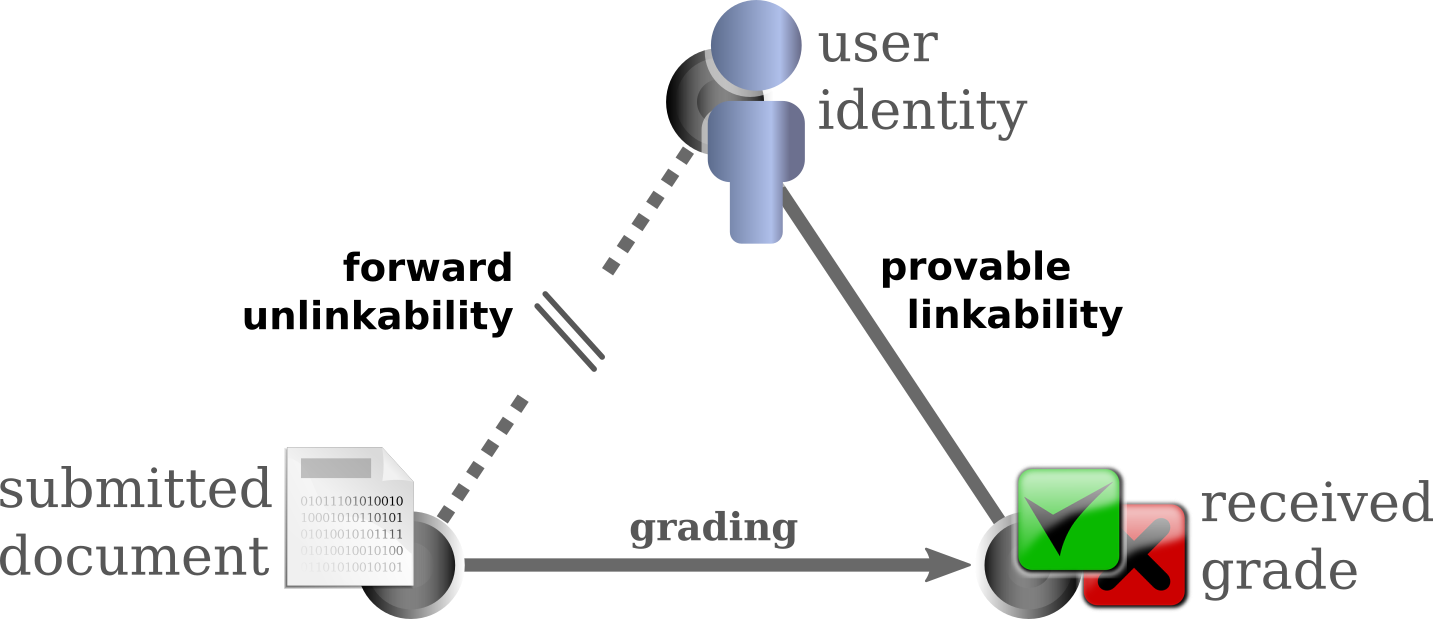
\includegraphics[width=0.5\textwidth]{images/document-submission-system/user-grade-document.png}
   \caption{Overview of system entities, their relations and desired properties.}
   \label{figure:document-submission-system:user-grade-document}
\end{figure}


Using the cryptographic technique of blind signatures
\cite{chaum_blind_1982}, we propose a protocol for this use case: a
privacy-preserving document submission and grading system that allows
students to submit documents anonymously without compromising the
correctness of the grade assignment process. 

%that guarantees perfect forward unlinkability of submitted documents and
%user identities for the students while at the same time provides a
%reliable linking of student identities to grades based on a blind
%grading process of the submitted documents.

After presenting related work in \Cref{section:document-submission-system:related-work}, we formulate a
system model and desired properties for the system in
\Cref{section:document-submission-system:anonymous-document-submission-system}. In
\Cref{section:document-submission-system:design-implementation} we suggest a protocol design that meets
these requirements, and evaluate the proposed protocol, discussing its
privacy and security properties in \Cref{section:document-submission-system:evaluation}. Furthermore,
we show the practical feasibility of the proposed solution by having
implemented a proof-of-concept prototype of the protocol, briefly
described in the same section.
    
%% contributions:
%\begin{itemize}
%
%    \item We describe a practical use case for applying blind signature
%        schemes to improve user privacy.
%
%    \item We design a protocol for a
%        document submission and grading system that guarantees perfect forward
%        unlinkability of submitted documents and user identities
%        while at the same time provides a reliable linking of
%        student identities to grades based on a blind grading
%        process of the submitted documents. 
%
%    \item We show the practical feasibility of the proposed solution by
%        implementing a proof-of-concept prototype of the protocol.
%
%    \item We evaluate the proposed protocol, discussing its privacy and
%        security guarantees and limitations.
%
%\end{itemize}


\section{Related Work}
    \label{section:document-submission-system:related-work}
%Anonymity and unlinkability are popular capabilities addressed in current literature 
%for similar problems. The former commonly resolved with the aid of onion routing 
%implementations \cite{dingledine_tor_2004}, while the latter has seen different solutions, 
%\eg blind digital signatures schemes \cite{chaum_blind_1982}.

Blind signatures schemes are widely used to
enhance the privacy of protocols by providing unlinkability. Examples 
of their use include identity management in federated login systems, \eg PseudoID 
\cite{DeyW10}, a project to protect the login data from the identity providers by 
means of blind digital signatures, 
or electronic payment systems, \eg \acs{taler} \cite{inria15}, a digital currency approach 
close to Bitcoin with the additional benefit of governmental tax traceability
without losing anonymity as blind signatures provide unlinkability to the transactions 
between customers and merchants but not between government and merchants. 
Secure voting schemes are another application area of blind signatures, 
\eg CryptoBallot \cite{Hayes13}, a cryptographically secure online voting system 
where ballots cannot be traced back to the voter as they are blinded but their counting 
and the voter identities are publicly auditable. Even though these
schemes have similarities with our problem, they would be unnecessarily
complex to adapt for the use case of document submission and grading.
%
%Smart-card technologies have been used to store credentials for identity management. 
Attribute-based anonymous credentials can be used for similar purposes,
such as in an anonymous course evaluation system for universities
\cite{StamatiouBGKLPT15}. The use-case of this project differs, however,
from our problem statement, having a focus on smart-card based anonymous
course attendance verification, introducing complexity not needed in our
scenario.
%
%The project \Ac{irma} aims at attribute-based identity 
%management in a privacy-preserving manner by storing the credentials in the smart-card 
%though these are not anonymous \cite{AlparH13}.
%
Whistleblower platforms, \eg SecureDrop \cite{fpf13} or
GlobaLeaks \cite{Hermes11}, allow a sender to submit documents
anonymously to a receiver, such as a media organization. These systems
employ anonymous and confidential communication and meta-data footprint
minimization to increase the anonymity of the sender. While maximizing
the sender anonymity, they lack, however, the provable linkability
of feedback (grades in our scenario) to identifiers, that is required in
our use case.

%
%To the best of our knowledge there is no anonymous, privacy-preserving
%system or platform allowing the submission of documents and grading with
%the functionality and properties we require, of applicability in our
%considered context.



% \section{\Acl*{adss}}
\section{Anonymous Document Submission System}
    \label{section:document-submission-system:anonymous-document-submission-system}

We aim to design a document submission and grading system, 
%that allows
%students to submit documents anonymously and at the same time to
%claim the grade they got for their submitted work. 
%
% system model
%\subsection{System Model and Assumptions}
where each student can submit a document to the system before a public
deadline. After the deadline passed, the teacher %\footnote{Without loss of generality, we assume that there is only one teacher.} 
grades all submitted
documents with either pass or fail. When all documents are graded, each
student receives the grade that the teacher assigned to the document
that was submitted by the student.

% assumptions
%\subsection{Assumptions}
We assume that students can store credentials they receive in a secure
way, do not pass them on to others and that they can communicate with
the system in a mutually authenticated and confidential way (\eg via a TLS
secured web login), and at other times in an anonymous and confidential 
way (\eg by using TLS over \acs{tor}\cite{dingledine_tor_2004}).
We assume that they are careful to include no identifying information in
the documents and that authorship attribution by stylometry is not
feasible for the adversary.
When discussing the security and reliability of the system from the
teacher's perspective, we assume that the server cannot be compromised
and that the teacher can handle secret keys in a secure way.
Furthermore, protection against ghost writing is out of scope of this
work, so we assume that students will not ask someone else to write
their documents, which reflects a general limitation for home
assignments that are allowed to be worked on outside a
teacher-controlled environment.
%
% required properties
%\subsection{Required Properties}
To achieve anonymity and correctness, we want the system to have the
following two properties:
	
\begin{propertydef}[student--document forward unlinkability]
A document cannot be linked to a student by anyone else than the
student who submitted the document, and the unlinkability remains
even after grades have been assigned to students.
\end{propertydef}
\vspace{-1em}
\begin{propertydef}[student--grade provable linkability]
If and only if a document was graded with a certain grade, the
student who submitted the document can prove that she received
this grade.
% note that these are two directions, left to right: all passed students can prove (completeness), right to left: only passed students can prove (soundness)
\end{propertydef}

%threat model
%\subsection{Threat Model}
We want our system to both protect the student's privacy and to protect
the teacher from dishonest students. Therefore we consider two different
adversaries. 
%
The first adversary tries to break the student's anonymity and is
capable of compromising any involved party except for the student
herself. In particularly it can control the teacher, the server and any
other student. Furthermore, we assume this adversary to be capable to
passively intercept all network traffic and actively inject messages. 
%The only restriction is, that this adversary must not be able to observe
%the network traffic of the anonymous channel when it is originating from
%the student's device, as otherwise end-to-end traffic correlation
%attacks against practical anonymous communication tools such as \Ac{tor}
%will become possible.
%
The second adversary tries to break the correctness of the grade
assignment and is used when discussing the security and reliability of
the system from the teacher's perspective. 
This adversary is assumed to be able to compromise one student, to
passively observe all network traffic and to actively inject messages.


\section{Protocol Design}
    \label{section:document-submission-system:design-implementation}
We implement the protocol that has the desired properties using a blind
signature scheme as described in \cite{chaum_blind_1982}, that provides the functions $blind, unblind, sign$ and
$verify$, with the property that blinding perfectly hides the data, but
signatures on blinded data can still be verified after unblinding
(informally: $unblind(sign(blind(x))) = sign(x)$).
%
\Cref{figure:document-submission-system:sequencediagram} shows the sequence of steps in our proposed protocol.
%
\begin{figure}[h!]
	\renewcommand{\msckeyword}{}
	\scriptsize
	\begin{msc}{}
		\setlength{\labeldist}{3ex}
		\drawframe{no}
		\declinst{student}{\parbox{3cm}{document $D$, teacher's \\public keys: $e_{pass},e_{fail}$}}{student}
		\declinst{server}{}{server}
		\declinst{teacher}{private keys: $d_{pass},d_{fail}$}{teacher}
		\setlength{\labeldist}{1ex}

		\action*{\parbox{5cm}{
			generate random $rID$ for each student
		%\\	store mappig of $rID$ to student-identifier
		}}{server}
		\nextlevel[3]

		\mess{$rID$}{server}{student} 
		\mess{\parbox{3cm}{\tiny (mutually authenticated, \\encrypted channel)}}[b]{server}{student} 
		\nextlevel[1.7]

		\messarrowscale{0}
		\mess*{\tiny done distributing $rID$s to all students}[b]{envleft}{envright}
		\messarrowscale{1.2}
		\nextlevel[1]

		\action*{\parbox{5cm}{
			generate random $b_{pass}$, $b_{fail}$\\
			$bID_{pass} = blind(rID,b_{pass},e_{pass})$\\
			$bID_{fail} = blind(rID,b_{fail},e_{fail})$
		}}{student} 
		\nextlevel[4.5]

		\mess{$D,bID_{pass},bID_{fail}$}{student}{server} 
		\mess{\tiny (anonymous, encrypted channel)}[b]{student}{server} 
		\nextlevel[1.5]

		\messarrowscale{0}
		\mess*{\tiny hand-in deadline}[b]{envleft}{envright}
		\messarrowscale{1.2}
		\nextlevel[1]

		\setlength{\inlineoverlap}{22mm}
		\inlinestart{grading}{for all submitted documents}{server}{teacher}
				\nextlevel[2.5]

				\mess{$D,bID_{pass},bID_{fail}$}{server}{teacher} 
				\nextlevel[1]

				\action*{\parbox{40mm}{
					$sbID = sign(d_{pass},bID_{pass})$ or\\
					$sbID = sign(d_{fail},bID_{fail})$
				}}{teacher} 
				\nextlevel[3]

				\mess{$sbID$}{teacher}{server} 
				\nextlevel[1]
		\inlineend{grading}
		\nextlevel[1.5]

		\mess{list of all $sbID$s}{server}{student} 
		\nextlevel[1]

		\action*{\parbox{50mm}{
						$sID = unblind(sbID,b_{pass},e_{pass})$ or\\
						$sID = unblind(sbID,b_{fail},e_{fail})$ 
		}}{student}
		\nextlevel[3.5]

		\mess{$rID, sID$}{student}{server} 
		\nextlevel[1]

		\action*{\parbox{50mm}{
						check if $sID == sign(d_{pass},rID)$\\
						or $sID == sign(d_{fail},rID)$.\\
						Register grade for student with $rID$.
		}}{server}
		\nextlevel[3.5]

	\end{msc}

	\caption{Protocol realizing an anonymous document submission and grading system.} 
	\label{figure:document-submission-system:sequencediagram}
\end{figure}%
%
First, the system server provides each registered student in the course
with a unique, random, one-time identifier $rID$ and stores the relation
of student identifiers to $rID$s for later use.
%timing attack!: distribution has to be completed before first submission!
%cutting%Distributing the $rID$s instead of using public, permanent student
%identifiers such as e-mail addresses or social insurance numbers
%avoids impersonation and replay attacks.  
Next, the student blinds the $rID$ for both the pass verification key
$e_{pass}$ and the fail verification key $e_{fail}$, using two private,
random blinding factors $b_{pass}$ and $b_{fail}$, and sends the
resulting $bID_{pass} = blind(rID,b_{pass},e_{pass})$ and $bID_{fail} =
blind(rID,b_{fail},e_{fail})$ together with $D$, the document to submit,
to the server over an anonymous, encrypted channel. %, \eg by using TLS over Tor.
%crypto attack!: we need to use two different blinding factors b if we blind the same rID for two different public keys! Otherwise the server can construct two public keys epass and efail with same modulus n and for which it holds that epass-efail=1, then the server can divide the two blinded ids and by this obtain b, because bID_pass / bID_fail = (b^epass * rID) / (b^efail * rID) = b^(epass-efail)
At this point, the server does not learn who submitted the document
because the blinding hides the $rID$, using the anonymous channel
obfuscates the network address origin and the document $D$ is assumed
to not contain any identifying information about the student.
%timing attack!: students should use home network, not university network to avoid Tor entry-exit-node correlation attacks! [as pointed out by Tobias]
After the deadline has passed, the teacher grades all submitted documents.
If a document is graded as passed, the
blinded identifier $bID_{pass}$ that was submitted together with the document
is signed with the private pass signing key $d_{pass}$ of the teacher. If the grade is fail, $bID_{fail}$
will be signed with the teacher's private fail signing key $d_{fail}$.
When all documents are graded, the server publishes a list of all signed
blinded identifiers. 
The student fetches the list, picks the signed blinded identifier that
belongs to her and unblinds it. 
The student will try both public verification keys $e_{pass}$ and $e_{fail}$
to check which grade she received. 
%She will also need to try all signed blinded identifiers in the list from the server, as they do not contain identifying information, but the protocol could easily be extended to have a student-chose pseudonym attached to both the submission and the list (eg a hash of $D$).
By this, the student obtains a signed identifier $sID = sign(rID)$
that proves that she received the grade corresponding to
the signing-key.
Finally, she sends $sID$ to the server, the server checks the signature,
looks up the student identifier that belongs to $rID$, and registers the
corresponding grade for the student, not learning which document the
student submitted.

%\subsection{Other Grading Scales and Submission Acknowledgements}
%
%The basic protocol as outlined above can be extended in different ways
%to incorporate more features and functionality. 
%
%The grading scale can easily be extended to any discrete scale, \eg an
%A-F scale instead of the pass/fail scale considered so far, by
%introducing more grade keys. Instead of having only the
%$e_{pass},d_{pass}$ and $e_{fail},d_{fail}$ keypairs, the teacher would
%generate and publish one keypair per grade, use them accordingly during
%grading and the students would check the signed blinded results against
%all of them. This comes, however, with the disadvantage of smaller
%anonymity sets as they depend on the number of other students that
%received the same grade, as discussed later in the evaluation.
%
%Another useful functionality is the acknowledgement of submissions by
%the server, so that in the case of a technical failure that causes a
%document not to be graded, the student still has a mean to prove that
%she handed in a document before the deadline. A straightforward implementation
%of this would be that the server signs each submitted document immediately
%with an extra key for that purpose, a ``handed-in key''. If later the
%student discovers that there is no entry for her in the result list,
%she can choose to give up her anonymity and present the signed document
%to the server, proving that she handed it in before the deadline.
%
%%oldTODO: extension: submission acknowledgement (simple solution: server returns signature (with extra hand-in key) on D upon submission, drawback: student has to give up anonymity for claiming it (maybe do another round of grading without giving up anonymity by only accepting signed documents for this second round, but what if result still incomplete after this round? maybe there's some cool zero-knowledge proof based solution for that, or secure mixing based solution would solve that?)
%
%% acknowledgement solution: by signing with a handed-in-key, but 
%% have to be thought through more, because students can cheat by presenting the 
%% acknowledgement and not claiming their grade
%
%%oldTODO: another extension: multiple grades (or in evaluation?)

\section{Discussion and Evaluation}
    \label{section:document-submission-system:evaluation}
%TODO: fix same-blinding-factor-deanonymization attack in implementation!
We have implemented a proof-of-concept prototype (see \url{http://www.ter.se/dss/}) %\footnote{The code of the prototype is available at http://www.ter.se/dss/}, 
which is a collection of C programs 
for the various operations performed by the student, server and teacher, realizing 
the described protocol. The prototype uses the free cryptographic library \texttt{Libgcrypt} \cite{fsf07}. 
% negligible performance issues, even on constraint devices
%
In the following, we do an informal security and privacy evaluation,
discussing why the previously defined properties hold and various
attacks will not succeed. We do not cover implementation-based attacks
though, such as cross-site-scripting attacks on a web-interface.

\paragraph{Student--document forward unlinkability}
%forward unlinkability: only k-anonymity among the other students with the same grade
The student identity is directly linked to the random identifier $rID$. 
But when submitting the document $D$, the $rID$ is perfectly hidden by the
random blinding factors known only to the student.
We assume that there is no identifying information contained in the
document, so after submission the server cannot link
student identifiers to documents.
To achieve forward unlinkability, this has to hold even after the grades
have been assigned to students.  
During grading, documents are linked to grades, which is a binary domain in our
case. The grade information is attached to the blinded $rID$ in form of 
a signature with one out of two keys, that can be transformed in a verifiable
signature on the unblinded $rID$ only by the student. The properties of the
blind signature scheme provide the unlinkability between this unblinded
signature and the blinded data that was submitted together with the document.
At the same time, the signature is provided to the server together with the $rID$ 
when the students claim their grades, so they provide an unambiguous
mapping from every $rID$ to a grade. As a consequence, we do not get
perfect unlinkability of student identifiers and documents, but only
\emph{k-anonymity}, where $k$ is the number of students who received the same
grade. This is a general limitation of every system where the grading
party is not trusted and the assignment of grades to student identifiers 
is verifiable. A worst-case example is a situation
where only one student received the grade ``fail'', so the
teacher can infer that the only document she graded with ``fail''
must belong to this student.
Another limitation is the fact, that the anonymity for all students with
a certain grade is reduced whenever one student with the same grade
gives up their anonymity voluntarily or becomes compromised by the
adversary.


\paragraph{Student--grade provable linkability}
% two directions
The provable linkability of student identifiers to grades has two
directions: (a) soundness: if a student can prove that she received a certain
grade, then she must have submitted a document that was graded
accordingly, and (b) completeness: if a document submitted by a student was graded
with a certain grade, then the student can prove that she received that
grade. 
%
We show (a) by contrapositive, so we assume that the student did not
submit a document that was graded with the grade that the student
claims. Now we see that the student cannot prove that she received
that grade: she cannot present a valid signature on the $rID$
assigned to her, made with the private key corresponding to the grade,
because the private signing key was used by the teacher only to sign
other blinded $rID$s that were submitted together with documents that
were graded accordingly.
%
For (b) we see directly that if a submitted document was graded with a
certain grade, the teacher put a signature on the blinded $rID$
submitted together with the document and publishes that later on. So the
student can derive a valid signature on her $rID$ by unblinding the
published information and therefore can prove to anyone knowing the
public verification key, that she received that grade.


\paragraph{Timing and Correlation Attacks}
% importance of deadlines (after rID handout, hand-in deadline/bulk-download of result)
To avoid timing attacks, it is important that certain events in the
protocol do not happen before others. For example, the hand-in of
documents must not start before all students received their $rID$s
(denoted by the first dashed line in the message sequence chart in
\Cref{figure:document-submission-system:sequencediagram}), otherwise the anonymity set for the
submitting students is immediately reduced to those who already received
their $rID$. 
For a similar reason it is important that the server publishes the
result list with the signed, blinded $rID$s after the hand-in deadline
and as a complete list. The latter is important, because if students for
example would request their individual entries without downloading the
complete list, the server could correlate these requests for specific
entries (that the server can link to documents) with requests for
registering a grade (which contain the identifier $rID$), that might
happen shortly after each other.
%
% Tor end-to-end traffic correlation attack (Tobias' comment)
End-to-end traffic correlation attacks are also relevant for the concrete
implementation of the anonymous channel. \acs{tor}, for example, does not
protect against an adversary that can observe both traffic going into
the \acs{tor} network and traffic coming out of it \cite{dingledine_tor_2004},
so the students should for example be advised not to use the university
network when submitting their documents, because it is likely that the
same party operates both the university network and the system server
and therefore could observe both ends of the students' connections.


\paragraph{Impersonation and Replay Attacks}
%importance of using $rID$ and not a public student id
To avoid impersonation and replay attacks, it is important not to use a
public or permanent student identifier such as the students' e-mail
addresses. Otherwise, an attacker could
impersonate a student, \eg to damage her reputation by submitting
a low-quality document in her name. Therefore, we use the 
unique, random, one-time identifier $rID$ and distribute it over a
mutually authenticated and encrypted channel to the student. This makes 
impersonation without the cooperation of the student impossible because
the attacker does not know which $rID$ was assigned to a 
student. It also prevents replay attacks,
as the $rID$ binds the messages both to the student and to the 
current course, because even if the same protocol is used for several
courses, the same student will receive a new $rID$
in each new protocol run.

\paragraph{Attacks on Combined Cryptographic Primitives}
% won't discuss them really but refer to papers (double-check attacks on RSA paper)
% discuss shared-blinding-factor attack
Attacks on the used cryptographic primitives, such as public key
cryptography, hash functions and blind signatures, are out
of scope of this work, so we assume them to be secure. However, we have
to be careful to use these tools in a secure way, especially when
combining them with each other. It is, for example, important to use two
different blinding factors $b_{pass}$ and $b_{false}$ when blinding the
$rID$.  Otherwise, if for ease of implementation one would use only one
common blinding factor $b$ for both blindings, the server would be able
to mount the following de-anonymization attack: 
%
\newcommand{\modn}{\ensuremath{\quad(\mathrm{mod}\ N)}}
The server generates specially prepared public keys $e_{pass} = \langle
N,e \rangle$ and $e_{fail} = \langle N,e' \rangle$ with the property
that both share the same modulus $N$ and the public exponents have a
difference of one: $e - e' = 1 \modn$.
%For example generating e_pass normally and then setting e_fail =
%(e_pass-1,n). The latter will be an invalid public key (in the sense
%that the DSS does not have a corresponding private key to it), but as
%long as the student does not check for these properties the attack works.
If the student blinds her $rID$ for these keys using a common blinding
factor $b$, she will submit the following two values to the server:
$bID_{pass} = blind(rID,b,e_{pass}) = rID \cdot b^{e} \modn$,
$bID_{fail} = blind(rID,b,e_{fail}) = rID \cdot b^{e'} \modn$.
Now, the server can simply divide the two values to obtain the blinding
factor $b$:
$bID_{pass} / bID_{fail} = (b^{e}\cdot rID) / (b^{e'}\cdot rID) =
b^{e-e'} = b \modn$.
Having learned $b$, the server can unblind the $bID$s and obtain $rID$,
thus having de-anonymized the student.



%\paragraph{System Implementation Attacks}
%Attacks on the used system components are also out of scope of this work.
%So we simply assume that there are no web-security flaws that allow for
%common attacks such as cross-site-scripting or
%cross-site-request-forgery on the server side interface, that injection attacks on
%the server's database are prevented, that secure
%versions of TLS are used for the authenticated channels and the involved
%certificate authorities are not compromised, that \Ac{tor} is used in a secure
%way to avoid side-channels attacks such as browser fingerprinting, that
%students use secure devices to prevent leakage of their credentials and
%that the system usability facilitates a secure usage.
%Even though these threats are out of scope of this work, they are
%important in practice and have to be taken into account when
%implementing an actual system.


\section{Conclusions and Limitations}
    \label{section:document-submission-system:conclusions-future-work}
%Blind signature schemes are a standard cryptographic technique used for example
%in digital currencies or voting schemes, where a user signs a message without
%being able to know the content of the message.

We have described a practical application for blind signatures schemes in the context 
of a document submission and grading system to 
improve the privacy of students without undermining the correctness 
of the grading process.
%
%We formulated two main required properties,
%student--document forward unlinkability (to protect the students' privacy even after the 
%grading process) and student--grade provable linkability (to guarantee that a certain 
%grade can only be claimed by a student who submitted a document with such grade),
%and designed a protocol that guarantees these properties.
%
%Our protocol specification has been implemented in a proof-of concept
%prototype using the standard cryptographic library \texttt{Libgcrypt},
%and we carried out a security and privacy evaluation of the protocol
%showing how the defined properties hold. We also analysed how different
%types of attacks, such as timing, correlation, impersonation and replay
%attacks are prevented. Moreover, we discussed the importance of careful
%protocol design when combining cryptographic primitives by providing an
%example for a seemingly innocent implementation simplification that
%actually introduces a vulnerability for a complete de-anonymization
%attack.
%
We found that it is feasible to implement such a
system, qualified
only by the limitations derived from the scenario, \eg that the provided
$k$-anonymity depends on the number of other students who received the
same grade, that students can choose not to reveal their grade, and that
documents cannot be linked to students even where this might be desired
for pedagogical reasons or penalty measures for plagiarism
that go beyond grading the work with fail.
%

The basic protocol described here can be extended with more
functionality such as having several teachers do the grading, using more
fine grained grading scales (with the limitation that this decreases the
anonymity sets), issuing submission acknowledgements or including
individual feedback without breaking the anonymity properties.

%future work
%For future work we want to look at the trade-off of anonymity and
%accountability, for example systems with a limited trusted third party,
%so that documents can be linked to identifiers in case of plagiarism or
%other disputes. Furthermore, we plan to explore the applicability of
%anonymous attribute-based credentials to enrich the functionality of the
%system, for example to include anonymous credentials for having met
%prerequisites of a course.
%A formal proof of the security and privacy aspects of our protocol is
%another goal of future work that would provide stronger guarantees
%compared to the privacy and security evaluation conducted in this paper.
%Finally, we aim for developing a secure and usable application from the
%prototype that can be used in practice for a university course.

% nice-to-have: Find Ian Goldberg's reference for delay idea (to mitigate network monitoring) [also read up on different solutions for this same problem: Mixmaster and Mixminion, referenced in https://blog.torproject.org/blog/traffic-correlation-using-netflows ]


\section*{Acknowledgments}
    \label{section:document-submission-system:acknowledgments}
This research has been funded by the \Acl{ssf} grant SSF FFL09-0086 and the \Acl{vr} 
grant VR 2009-3793.


%%%%%%%%%%%%%%%%%%%%%%%%%%%%%%%%%%%%%%%%%%%%%%%%%%%%%%%%%%%%%%%%%%%%%%%%%%%%%%%
%In the bibliography, use \texttt{\textbackslash textsuperscript} for ``st'', ``nd'', ...:
%E.g., \enquote{The 2\textsuperscript{nd} conference on examples}.

% \bibliographystyle{utils/splncs03}
% \bibliography{ppsds}

%%%%%%%%%%%%%%%%%%%%%%%%%%%%%%%%%%%%%%%%%%%%%%%%%%%%%%%%%%%%%%%%%%%%%%%%%%%%%%%

% \end{document}

\newenvironment{quote_tos}{%
    \definecolor{formalshade}{rgb}{0.95,0.95,1}
    \setlength{\parindent}{0pt}
    \def\FrameCommand{%
        \hspace{1pt}%
        {\color{DarkBlue}\vrule width 2pt}%
        {\color{formalshade}\vrule width 4pt}%
        \colorbox{formalshade}%
    }%
    \MakeFramed{\advance\hsize-\width\FrameRestore}%
    \noindent\hspace{-4.55pt}% disable indenting first paragraph
    \begin{adjustwidth}{}{7pt}%
        \vspace{2pt}\vspace{2pt}%
}
{%
    \vspace{2pt}\end{adjustwidth}\endMakeFramed%
}

\cleardoublepage
% \phantomsection
% \appendix
% \addcontentsline{toc}{part}{Appendices}
\bookmarksetupnext{level=-1}
% -*- mode: TeX -*-
% -*- coding: utf-8 -*-

\begin{appendices}
    \addappheadtotoc
    %\appendixpage
    \renewcommand\thechapter{\greek{chapter}}
    \renewcommand\thesection{\thechapter.\greek{section}}
    \crefalias{section}{appsec}
    \crefalias{chapter}{appchp}

    %\chapter{Excerpts of \aclp*{tos} and \aclp*{pp}}
    \chapter{Excerpts of Terms of Services and Privacy Policies}
        \label{chapter:thesis:excerpts-of-tos-and-pp}
    
    % TODO: replace the word sections with a cleverref command
    \lettrine{\textcolor[gray]{.25}{I}}{n} the following \namecrefs{section:thesis:related-work} we quote some 
    selected excerpts of the \ac{tos} and \ac{pp} of a few \ac{osn} service providers 
    that we thought --- as computer scientists --- interesting to be aware of in 
    our realm of research.
    
    We include the last update date stated by the service provider of the \ac{tos} 
    and \ac{pp} as well as the corresponding \acp{url} where we originally found 
    the terms and policies --- however, the wording and even the \ac{url} are likely 
    to change at any time.

    \section[\Facebook]{\Facebook (\FacebookInc)}
        \label{section:thesis:excerpts-facebook}
    % \cite{Facebook15}
    \Facebook's \acs{tos} are called ``Statement of Rights and Responsibilities
    '' and available at \url{https://www.facebook.com/terms}. The last revision as of 
    this writing is dated on January 30th, 2015. The following is an excerpt of some 
    selected sections of the \ac{tos}.

    \begin{quote_tos}
        \[...\]
        \textbf{Privacy}

        Your privacy is very important to us. We designed our Data Policy to make important 
        disclosures about how you can use Facebook to share with others and how we collect 
        and can use your content and information. We encourage you to read the Data Policy, 
        and to use it to help you make informed decisions. 

        \vspace{\baselineskip}

        \textbf{Sharing Your Content and Information}

        You own all of the content and information you post on Facebook, and you can control 
        how it is shared through your privacy and application settings. In addition:

        \begin{enumerate}
            \item For content that is covered by intellectual property rights, like photos 
            and videos (IP content), you specifically give us the following permission, 
            subject to your privacy and application settings: you grant us a non-exclusive, 
            transferable, sub-licensable, royalty-free, worldwide license to use any IP 
            content that you post on or in connection with Facebook (IP License). This IP 
            License ends when you delete your IP content or your account unless your content 
            has been shared with others, and they have not deleted it.
    
            \item When you delete IP content, it is deleted in a manner similar to emptying 
            the recycle bin on a computer. However, you understand that removed content 
            may persist in backup copies for a reasonable period of time (but will not be 
            available to others).
    
            \item When you use an application, the application may ask for your permission 
            to access your content and information as well as content and information that 
            others have shared with you.  We require applications to respect your privacy, 
            and your agreement with that application will control how the application can 
            use, store, and transfer that content and information.  (To learn more about 
            Platform, including how you can control what information other people may share 
            with applications, read our Data Policy and Platform Page.)
    
            \item When you publish content or information using the Public setting, it means 
            that you are allowing everyone, including people off of Facebook, to access 
            and use that information, and to associate it with you (i.e., your name and 
            profile picture).
    
            \item We always appreciate your feedback or other suggestions about Facebook, 
            but you understand that we may use your feedback or suggestions without any 
            obligation to compensate you for them (just as you have no obligation to offer 
            them).
        \end{enumerate}
        \[...\]
    \end{quote_tos}

    \section[\LinkedIn]{\LinkedIn (\LinkedInCorp)}
        \label{section:thesis:excerpts-linkedin}
    % \cite{LinkedIn14}
    \LinkedIn's \acs{tos} are called ``User Agreement'' and available at \url{https://www.linkedin.com/legal/user-agreement}. 
    The last revision as of this writing is dated on October 23rd, 2014. The following 
    is an excerpt of some selected sections of the \ac{tos}.

    \begin{quote_tos}
        \[...\]
        \textbf{Your License to LinkedIn}
        
        As between you and LinkedIn, you own the content and information that you 
        submit or post to the Services and you are only granting LinkedIn the following 
        non-exclusive license: A worldwide, transferable and sublicensable right 
        to use, copy, modify, distribute, publish, and process, information and 
        content that you provide through our Services, without any further consent, 
        notice and/or compensation to you or others. These rights are limited in 
        the following ways:
        \begin{enumerate}[label=\alph*]
            \item You can end this license for specific content by deleting such 
            content from the Services, or generally by closing your account, except 
            (a) to the extent you shared it with others as part of the Service and 
            they copied or stored it and (b) for the reasonable time it takes to 
            remove from backup and other systems.
            \item We will not include your content in advertisements for the products 
            and services of others (including sponsored content) to others without 
            your separate consent. However, we have the right, without compensation 
            to you or others, to serve ads near your content and information, and 
            your comments on sponsored content may be visible as noted in the Privacy 
            Policy.
            \item We will get your consent if we want to give others the right to 
            publish your posts beyond the Service. However, other Members and/or 
            Visitors may access and share your content and information, consistent 
            with your settings and degree of connection with them.
            \item While we may edit and make formatting changes to your content 
            (such as translating it, modifying the size, layout or file type or 
            removing metadata), we will not modify the meaning of your expression.
            \item Because you own your content and information and we only have 
            non-exclusive rights to it, you may choose to make it available to others, 
            including under the terms of a Creative Commons license.
        \end{enumerate}
        You agree that we may access, store and use any information that you provide 
        in accordance with the terms of the Privacy Policy and your privacy settings.

        By submitting suggestions or other feedback regarding our Services to LinkedIn, 
        you agree that LinkedIn can use and share (but does not have to) such feedback 
        for any purpose without compensation to you.

        You agree to only provide content or information if that does not violate 
        the law nor anyone's rights (e.g., without violating any intellectual property 
        rights or breaching a contract). You also agree that your profile information 
        will be truthful. LinkedIn may be required by law to remove certain information 
        or content in certain countries.
        \[...\]
        \textbf{Limits}
        
        LinkedIn reserves the right to limit your use of the Services, including 
        the number of your connections and your ability to contact other Members. 
        LinkedIn reserves the right to restrict, suspend, or terminate your account 
        if LinkedIn believes that you may be in breach of this Agreement or law 
        or are misusing the Services (e.g. violating any Do and Don'ts).

        LinkedIn reserves all of its intellectual property rights in the Services. 
        For example, LinkedIn, SlideShare, LinkedIn (stylized), the SlideShare and 
        “in” logos and other LinkedIn trademarks, service marks, graphics, and logos 
        used in connection with LinkedIn are trademarks or registered trademarks 
        of LinkedIn. Other trademarks and logos used in connection with the Services 
        may be the trademarks of their respective owners
        \[...\]
    \end{quote_tos}

    \section[\Twitter]{\Twitter (\TwitterInc)}
        \label{section:thesis:excerpts-twitter}
    % \cite{Twitter16}
    \Twitter's \acs{tos} are called ``Twitter Terms of Service'' and available at 
    \url{https://twitter.com/tos}. The last revision as of this writing is dated 
    on September 30th, 2016. The following is an excerpt of some selected sections 
    of the \ac{tos}.

    \begin{quote_tos}
        \[...\]
        \textbf{Your Rights}
        
        You retain your rights to any Content you submit, post or display on or 
        through the Services. What’s yours is yours — you own your Content (and 
        your photos and videos are part of the Content).

        By submitting, posting or displaying Content on or through the Services, 
        you grant us a worldwide, non-exclusive, royalty-free license (with the 
        right to sublicense) to use, copy, reproduce, process, adapt, modify, publish, 
        transmit, display and distribute such Content in any and all media or distribution 
        methods (now known or later developed). This license authorizes us to make 
        your Content available to the rest of the world and to let others do the 
        same. You agree that this license includes the right for Twitter to provide, 
        promote, and improve the Services and to make Content submitted to or through 
        the Services available to other companies, organizations or individuals 
        for the syndication, broadcast, distribution, promotion or publication of 
        such Content on other media and services, subject to our terms and conditions 
        for such Content use. Such additional uses by Twitter, or other companies, 
        organizations or individuals, may be made with no compensation paid to you 
        with respect to the Content that you submit, post, transmit or otherwise 
        make available through the Services.

        Twitter has an evolving set of rules for how ecosystem partners can interact 
        with your Content on the Services. These rules exist to enable an open ecosystem 
        with your rights in mind. You understand that we may modify or adapt your 
        Content as it is distributed, syndicated, published, or broadcast by us and 
        our partners and/or make changes to your Content in order to adapt the Content 
        to different media. You represent and warrant that you have all the rights, 
        power and authority necessary to grant the rights granted herein to any 
        Content that you submit.
        \[...\]
    \end{quote_tos}
    
    \chapter{Creative Commons Legal Code}
        \label{chapter:thesis:creative-commons-legal-code}
        % hacks to hide the section and subsection commands that are issued as part of the \doclicenseFullText macro of the doclicense package
        \renewcommand{\section}[1]{%
            \par\refstepcounter{section}% Increase section counter
            \sectionmark{#1}% Add section mark (header)
            % \addcontentsline{toc}{section}{\protect\numberline{\thesection}#1}% Add section to ToC
            % Add more content here, if needed.
        }
        \renewcommand{\subsection}[1]{%
            \par\refstepcounter{subsection}% Increase subsection counter
            \subsectionmark{#1}% Add subsection mark (header)
            % \addcontentsline{toc}{subsection}{\protect\numberline{\thesubsection}#1}% Add subsection to ToC
            % Add more content here, if needed.
        }
        The following is the legal code for the \doclicenseLongNameRef~license created 
        by \Ac{cc}, a global non-profit organization whose mission is to enable the 
        ``sharing and reuse of creativity and knowledge through the provision of 
        free legal tools''.
        {
        % redefine the quotation environment to override the default format
        \renewenvironment{quotation}{%
            \definecolor{silver}{rgb}{0.83, 0.83, 0.83}
            \setlength{\parindent}{0pt}
            \def\FrameCommand{%
                \hspace{1pt}%
                %{\color{DarkBlue}\vrule width 2pt}%
                %{\color{formalshade}\vrule width 4pt}%
                \colorbox{silver}%
            }%
            \MakeFramed{\advance\hsize-\width\FrameRestore}%
            \noindent\hspace{-4.55pt}% disable indenting first paragraph
            \begin{adjustwidth}{}{0pt}%
                \vspace{2pt}\vspace{2pt}%
        }
        {%
            \vspace{2pt}\end{adjustwidth}\endMakeFramed%
        }
        \doclicenseFullText
        }

\end{appendices}


\cleardoublepage
\bookmarksetupnext{level=-1}
%\chapter*{References}
%\addcontentsline{toc}{chapter}{Bibliography}
\bibliography{data/bibliography}

\end{document}
% \endinput

